\documentclass[cs4size,a4paper,10pt]{ctexart}   

\linespread{1.5}
\usepackage{geometry}%用于设置上下左右页边距
	\geometry{left=2.5cm,right=2.5cm,top=3.2cm,bottom=2.7cm}
\usepackage{xeCJK,amsmath,paralist,enumerate,booktabs,multirow,graphicx,subfig,setspace,listings,lastpage,hyperref}
\usepackage{amsthm, amssymb, bm, color, framed, graphicx, hyperref, mathrsfs}
\usepackage{mathrsfs}  
	\setlength{\parindent}{2em}
	\lstset{language=Matlab}%
\usepackage{fancyhdr}
\usepackage{graphicx}
\usepackage{subfloat}
\usepackage{listings}
\usepackage{xcolor}
\usepackage{float}
\usepackage{paralist}
\usepackage{setspace}
\usepackage{titlesec}
\usepackage{enumitem}
\usepackage{hyperref}
\usepackage{multirow}
\usepackage{threeparttable}
\usepackage{autobreak}
\usepackage{multicol}
\usepackage{subfig}
\usepackage{unicode-math}
\usepackage{ltxtable, filecontents}
\usepackage{array}
\usepackage{amsmath}
\usepackage{pifont}
\usepackage{lipsum}
\usepackage{microtype}
\usepackage{wrapfig}
\usepackage[absolute,overlay]{textpos}
\usepackage{vwcol}

\hypersetup{
	colorlinks=true,
	linkcolor=black,
	urlcolor=black
}

\setenumerate{partopsep=0pt,topsep=0pt,itemsep=0pt,leftmargin=2em}
\setitemize{itemsep=0pt,partopsep=0pt,topsep=0pt,leftmargin=2em}

\titlespacing*{\section}{0pt}{3pt}{3pt}
\titlespacing*{\subsection}{0pt}{2pt}{2pt}
\titlespacing*{\subsubsection}{0pt}{1pt}{1pt}
\titlespacing*{\paragraph}{0pt}{0pt}{0pt}

\ctexset{secnumdepth=4,tocdepth=4}
\setlength{\parindent}{0pt}
\setstretch{1.3}

\setCJKmainfont[BoldFont={FZHei-B01},ItalicFont={FZKai-Z03}]{FZShuSong-Z01} 
\setCJKsansfont[BoldFont={FZHei-B01}]{FZKai-Z03} 
\setCJKmonofont[BoldFont={FZHei-B01}]{FZFangSong-Z02}
\setCJKfamilyfont{zhsong}{FZShuSong-Z01} 
\setCJKfamilyfont{zhhei}{FZHei-B01} 
\setCJKfamilyfont{zhkai}[BoldFont={FZHei-B01}]{FZKai-Z03} 
\setCJKfamilyfont{zhfs}[BoldFont={FZHei-B01}]{FZFangSong-Z02} 
\renewcommand*{\songti}{\CJKfamily{zhsong}} 
\renewcommand*{\heiti}{\CJKfamily{zhhei}} 
\renewcommand*{\kaishu}{\CJKfamily{zhkai}} 
\renewcommand*{\fangsong}{\CJKfamily{zhfs}}


\definecolor{mKeyword}{RGB}{0,0,255}          % bule
\definecolor{mString}{RGB}{160,32,240}        % purple
\definecolor{mComment}{RGB}{34,139,34}        % green
\definecolor{mNumber}{RGB}{128,128,128} 

\lstdefinestyle {njulisting} {
	basewidth = 0.5 em,
	lineskip = 3 pt,
	basicstyle = \small\ttfamily,
	% keywordstyle = \bfseries,
	commentstyle = \itshape\color{gray}, 
	basicstyle=\small\ttfamily,
	keywordstyle={\color{black}},     % sets color for keywords
	stringstyle={\color{black}},       % sets color for strings
	commentstyle={\color{black}},     % sets color for comments
	numberstyle=\tiny\color{black},
	numbers = left,
	captionpos = t,
	breaklines = true,
	xleftmargin = 1.2 em,
	xrightmargin = 0 em,
	frame=tlrb,
	tabsize=4,
	aboveskip = 7 pt, %与代码环境上一行的垂直间距
    belowskip = -2 pt %与代码环境下一行的垂直间距
}

\lstset{
style = njulisting, % 调用上述样式 
flexiblecolumns % 允许调整字符宽度
}

\renewcommand{\thefootnote}{\fnsymbol{footnote}}

\newcommand \sverb {\;\verb}
\definecolor{shadecolor}{rgb}{0.96,0.96,0.96}

%================= 基本格式预置 ===========================
\usepackage{fancyhdr}
\pagestyle{fancy}
\lhead{\textsc{SOA and Software Engineering}}
\rhead{面向服务的软件工程}
\cfoot{\thepage}
\renewcommand{\headrulewidth}{0.4pt}
\renewcommand{\theenumi}{(\arabic{enumi})}
\CTEXsetup[format={\bfseries\zihao{-3}}]{section}
\CTEXsetup[format={\bfseries\zihao{4}}]{subsection}
\CTEXsetup[format={\bfseries\zihao{-4}}]{subsubsection}

\renewcommand{\arraystretch}{1.23} %表格文字与表格线的距离

\renewcommand{\contentsname}{目录}  
\begin{document}

	\begin{center}
		{\huge\textbf{面向服务的软件工程}}
	\end{center}
	%---------目录---------% 
	\pagenumbering{Roman}
	\tableofcontents
	\clearpage

 	%---------正文---------% 
	\pagenumbering{arabic}
	\setcounter{page}{1}
	\setlength{\parskip}{0.45em}

	\setlength\abovedisplayskip{5pt}
	\setlength\belowdisplayskip{5pt}

	\section{服务与服务系统}

\subsection{服务}

\subsubsection{服务的概念}

\begin{itemize}
    \item 服务是为客户(担任协同提供者)所执行的非持久的,无形的体验。
    \item 服务是单个或一系列活动。这些活动或多或少带有无形的天然属性;这些活动通常(虽然不是必须)在客户和服务雇员/物理资源和产品/服务提供者的系统之间的交互中所发生。它们用来提供针对客户问题的解决方案。
\end{itemize}

服务的例子
\vspace{-0.8em}
\begin{multicols}{4}
    \begin{itemize}
        \item 传统物流仓储
        \item 信息咨询
        \item 金融、股票市场
        \item 租赁
        \item 科学技术服务
        \item 管理
        \item 娱乐
        \item ……  
    \end{itemize}
\end{multicols}
\vspace{-1em}

\subsubsection{服务与制造}

商品与服务的精确定义应根据其属性加以区分
\begin{itemize}
    \item 商品是可以创造和转让的有形实物或产品;它随着时间的推移而存在,因此可以在以后创建和使用。
    \item 服务是无形的,易变质的。它是同时或几乎同时创建和使用的事件或过程。虽然消费者在实际服务产生后无法保留,但服务的努力可以保留。
\end{itemize}

\begin{figure}[H]
	\setcounter{subfigure}{0}
	\centering
	\vspace{-0.5em}	
	\subfloat[Service vs.Manufacturing Model]{
	\begin{minipage}[c]{0.7\linewidth}
	\centering
	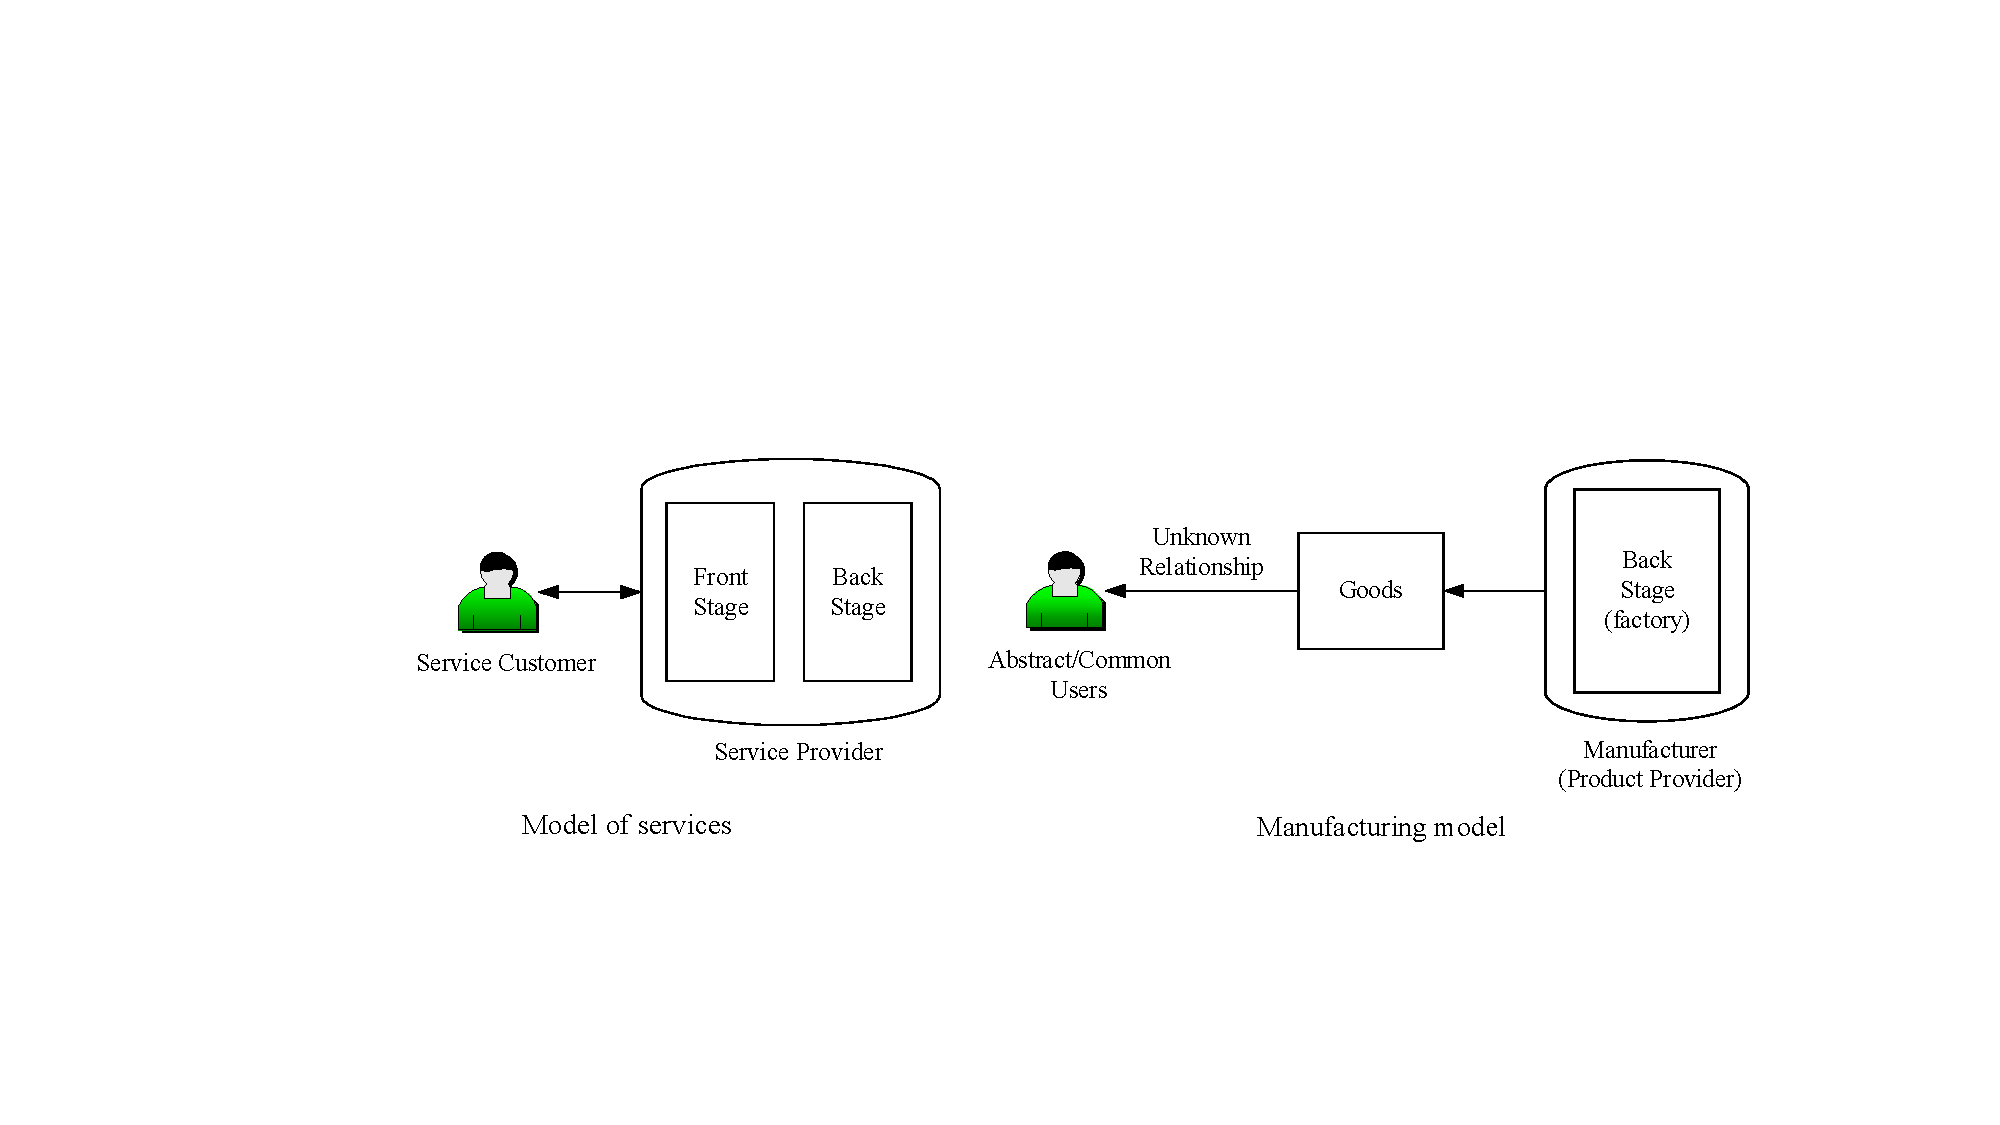
\includegraphics[width=0.97\linewidth]{images/Services vs Goods.pdf}
	\end{minipage}
	}
    \hfill
	\subfloat[Service-goods continuum]{
	\begin{minipage}[c]{0.25\linewidth}
	\centering
	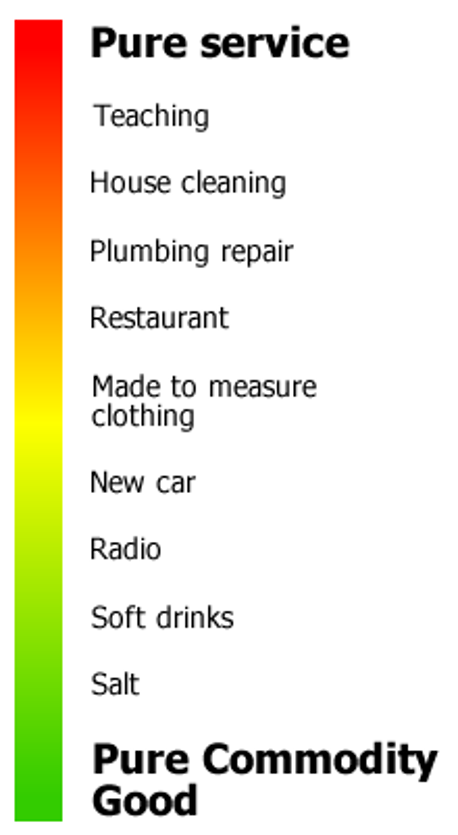
\includegraphics[width=0.9\linewidth]{images/Service-goods continuum.png}
	\end{minipage}
	}
	\centering
	\vspace{-1em}
\end{figure}

\subsubsection{服务发展趋势}
\vspace{-0.8em}
\begin{multicols}{2}
    \begin{itemize}
        \item 单纯的制造持续减少
        \item 服务产业持续增长
        \vspace{-0.8em}
        \begin{multicols}{3}
            \begin{itemize}
                \item 物业服务
                \item 安全保障
                \item 园艺
                \item 清洁工作
                \item 软件开发(外包)
            \end{itemize}
        \end{multicols}
        \vspace{-1.2em}
        \item 服务变得越来越复杂
        \begin{itemize}
            \item 银行的呼叫中心(业务支持系统)
            \item 提供医疗服务的医院(HIS)
            \item 复杂企业的管理(ERP, CRM, …)
            \item 电子银行或电子商务(B2C, B2B, …)
        \end{itemize}
        \item 引入各种IT系统
        \begin{itemize}
            \item 有没有服务雇员均可
        \end{itemize}
    \end{itemize}
\end{multicols}
\vspace{-1em}


\subsection{服务系统}

\subsubsection{基本概念}
服务系统是指用以实现业务服务的IT软件系统,相当多的软件系统是服务系统。

服务系统可以非正式定义为6元组
\vspace{-0.8em}
\begin{multicols}{3}
    \begin{itemize}
        \item 输入
        \item 输出
        \item 目标(内部目标,外部目标)
        \item 转换过程
        \item 组件
        \item 传感器
    \end{itemize}
\end{multicols}
\vspace{-1em}

其中组件包括
\vspace{-0.8em}
\begin{spacing}{1.12}
\begin{multicols}{2}
    \begin{itemize}
        \item 服务人员
        \vspace{-0.8em}
        \begin{multicols}{2}
            \begin{itemize}
                \item 设计人员
                \item 开发人员
                \item 测试人员
                \item ……
            \end{itemize}
        \end{multicols}
        \vspace{-1.2em}
        \item 服务伙伴
        \vspace{-0.8em}
        \begin{multicols}{2}
            \begin{itemize}
                \item 客户
                \item 服务雇员
            \end{itemize}
        \end{multicols}
        \vspace{-1.2em}
        \item 服务信息
        \item 服务步骤
        \item 服务基础架构资源架构(物理/IT/抽象)
    \end{itemize}
\end{multicols}
\end{spacing}
\vspace{-1em}

\begin{figure}[H]
	\setcounter{subfigure}{0}
	\centering
	\vspace{-0.5em}	
	\subfloat[Self Contained \& Encapsulated]{
	\begin{minipage}[c]{0.6\linewidth}
	\centering
	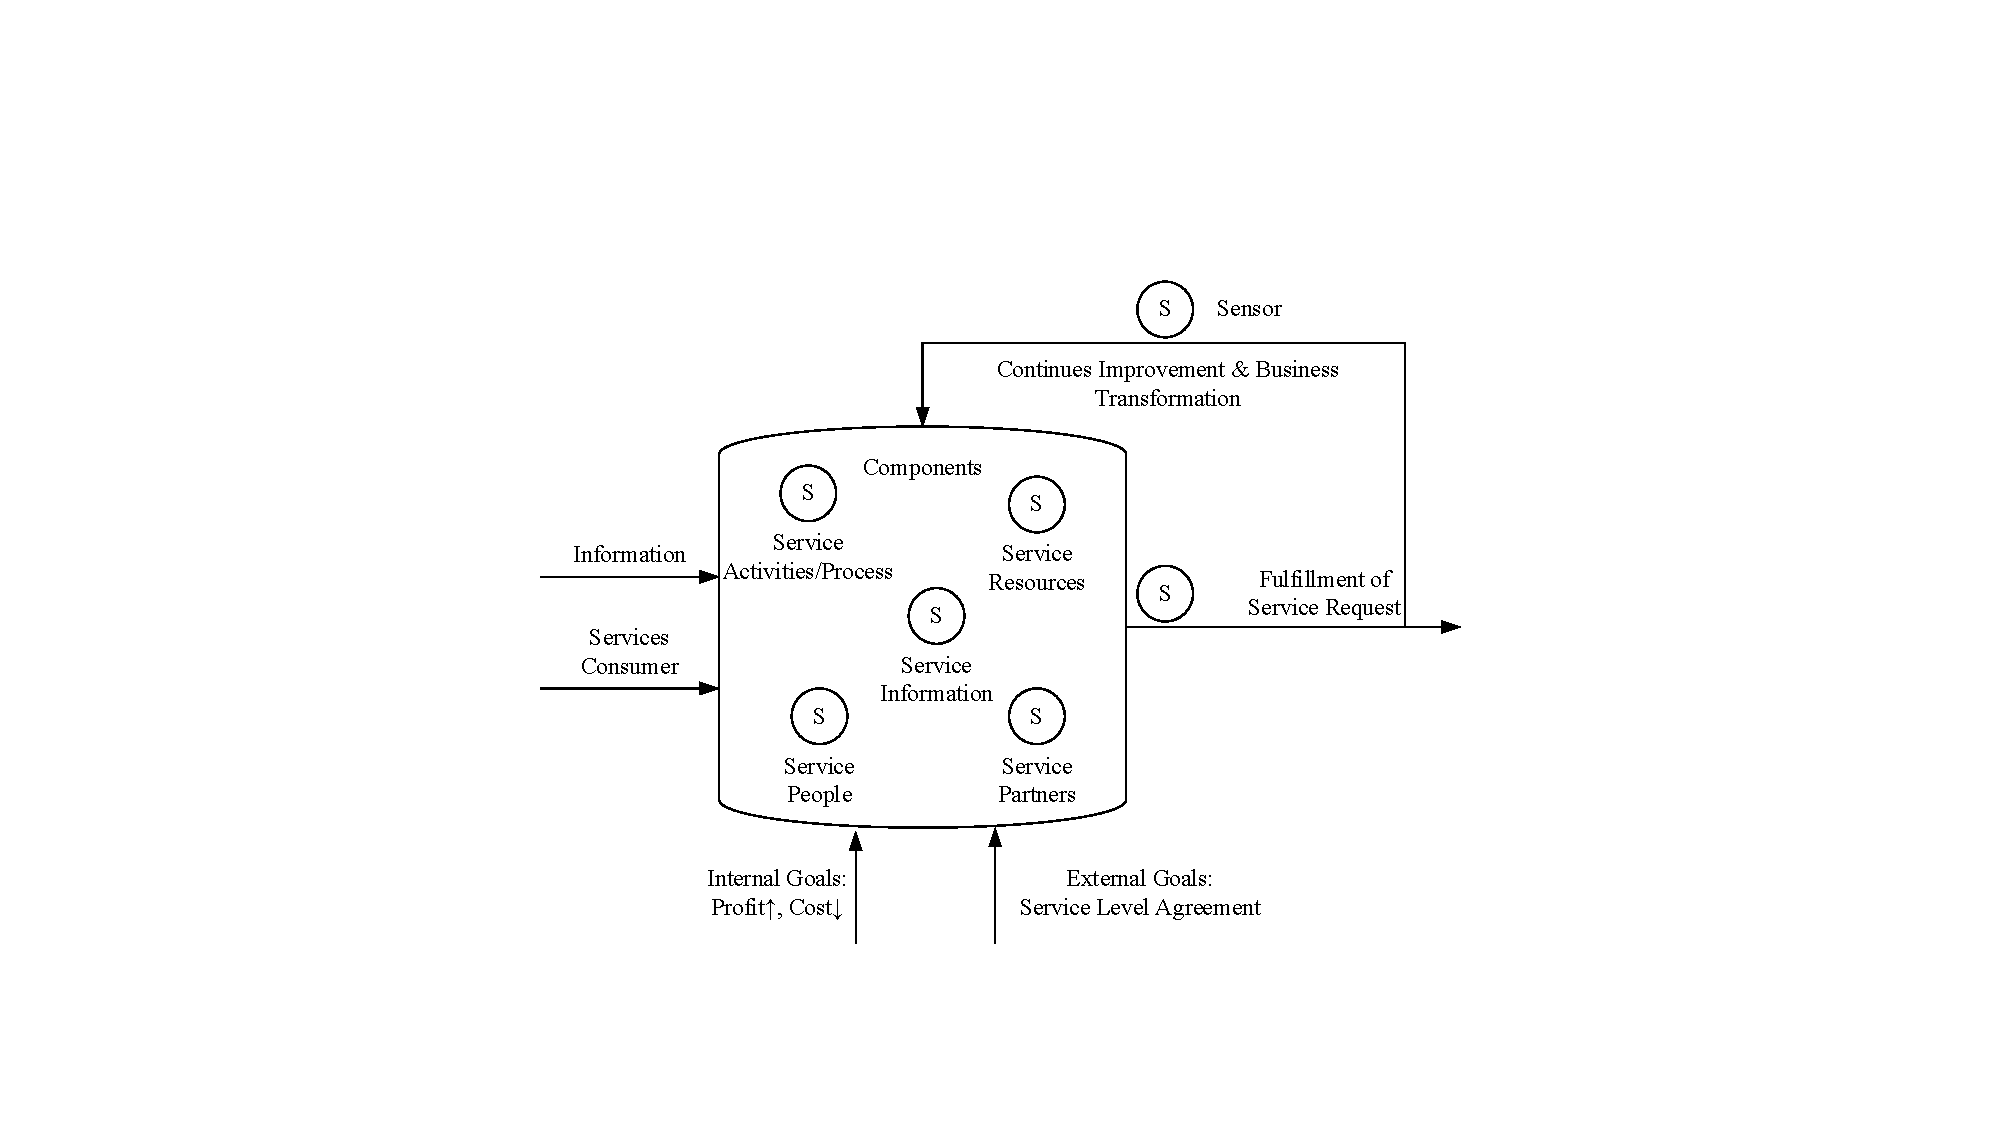
\includegraphics[width=0.97\linewidth]{images/Self Contained Encapsulated.pdf}
	\end{minipage}
	}
	\subfloat[服务系统的视角观点]{
	\begin{minipage}[c]{0.35\linewidth}
	\centering
	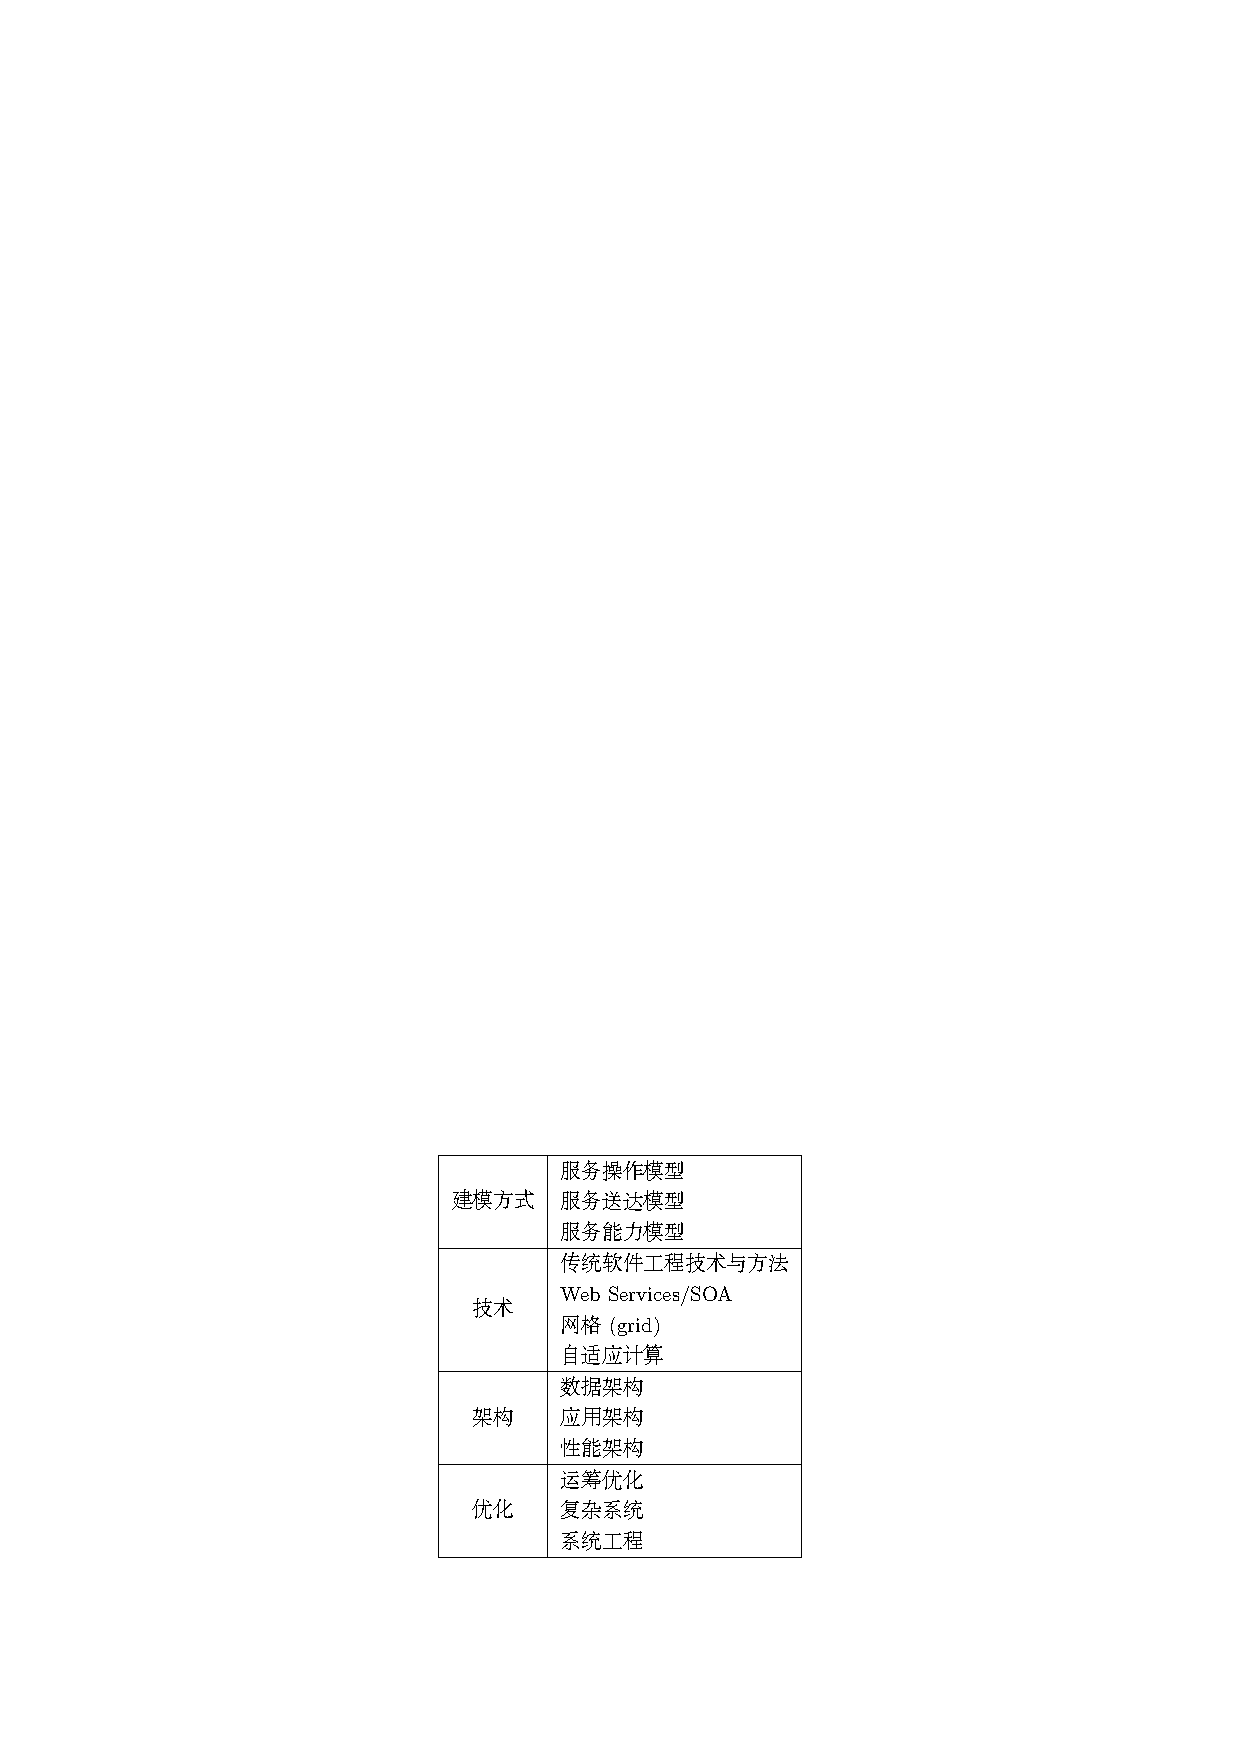
\includegraphics[width=0.97\linewidth]{images/服务系统的视角观点.pdf}
	\end{minipage}
	}
	\centering
	\vspace{-1em}
\end{figure}

服务系统遇到的问题和挑战
\vspace{-0.8em}
\begin{multicols}{2}
    \begin{itemize}
        \item 服务系统的复杂性
        \item 服务系统的灵活性
        \item 专业化和外包模式
        \item 计算环境的演化
        \item IT专家和业务专家之间的隔阂
        \item 新增价值和创新功能
        \item 一系列有着略微差异的服务系统(产品家族、产品线) 
    \end{itemize}
\end{multicols}
\vspace{-1em}

\subsubsection{IT使能的服务系统}
当业务服务由服务系统提供,该服务被称为IT使能的服务系统。

服务表示至少一个服务提供商和一个服务使用者之间为实现特定业务目标或解决方案目标而进行的基于关系的交互活动。

其中可能既含有IT服务,也可能含有非IT服务,区别包括:
\vspace{-0.8em}
\begin{multicols}{3}
    \begin{itemize}
        \item 关键绩效(KPIs)不同
        \item 需求管理不同
        \item 服务步调不同
    \end{itemize}
\end{multicols}
\vspace{-1em}

IT使能的服务系统具有2个特点:操作模型和收费模型

操作模型
\vspace{-0.8em}
\begin{multicols}{3}
    \begin{itemize}
        \item 点对点模型
        \item 集中服务模型
        \item 商务流程外包(BPO)
        \item 以数据为核心的外包(DCO)
        \item 通过在线经纪代理提供服务
    \end{itemize}
\end{multicols}
\vspace{-1em}

收费模型
\vspace{-0.8em}
\begin{multicols}{3}
    \begin{itemize}
        \item 免费模型
        \item 基于费用模式的模型
        \item 政府提供的公益模型
    \end{itemize}
\end{multicols}
\vspace{-1em}

\subsubsection{服务生态系统}
从客户视角来看,有许多服务可以同时独立使用
\vspace{-0.8em}
\begin{multicols}{2}
    \begin{itemize}
        \item 所以他们被叫做垂直服务
        \item 分为纯IT服务和IT支持服务
    \end{itemize}    
\end{multicols}
\vspace{-1em}

垂直服务可以用一些可复用的跨行业公共服务来构建
\vspace{-0.8em}
\begin{multicols}{2}
    \begin{itemize}
        \item 所以它们被称为水平服务
        \item 分为通用业务服务和IT服务
    \end{itemize}    
\end{multicols}
\vspace{-1em}

\begin{figure}[H]
    \vspace{-0.5em}
	\centering
	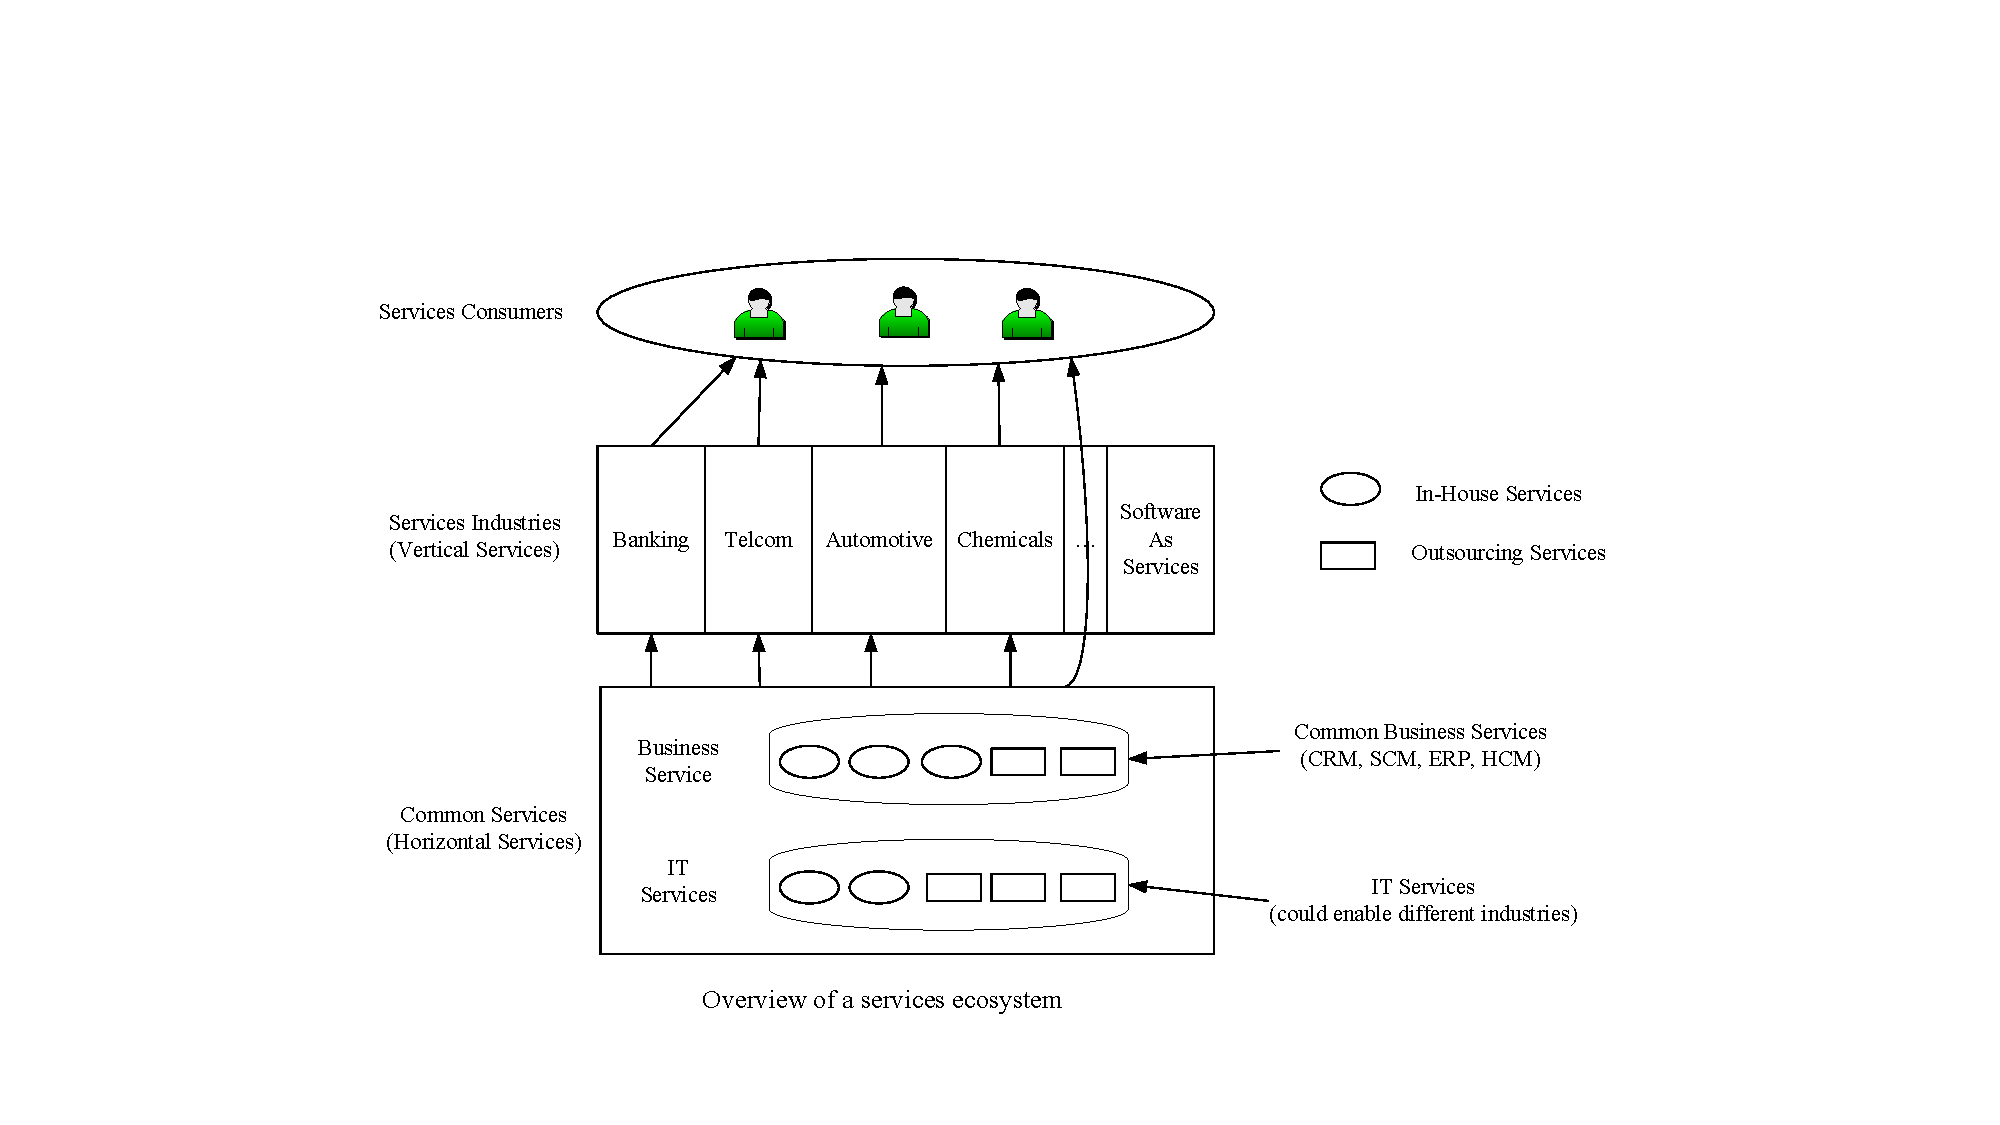
\includegraphics[width=0.85\textwidth]{images/Overview of a services ecosystem.pdf}
    \vspace{-1em}
\end{figure}

需要关注的问题有:
\vspace{-0.8em}
\begin{multicols}{2}
    \begin{itemize}[leftmargin=1em]
        \item 如何利用有限资源建立和维护适当的服务系统?
        \item 如何建立和维护适当的服务生态系统/服务库存?
    \end{itemize}   
\end{multicols}
\vspace{-1em}


\subsection{面向服务的范型}

\subsubsection{软件的发展过程}
\begin{itemize}
    \item 软件危机
    \vspace{-0.8em}
    \begin{multicols}{2}
    \begin{itemize}
        \item 用户需求不明确 
        \item 缺乏正确的理论指导
        \item 软件开发规模越来越大
        \item 软件开发复杂度越来越高 
    \end{itemize}  
    \end{multicols}
    \vspace{-1em}
    \item 服务系统的问题尤其突出
    \item 软件工程
    \vspace{-0.8em}
    \begin{multicols}{2}
    \begin{itemize}
        \item 软件过程及相关理论、方法和工具
        \item 软件产品簇、产品线
        \item \textbf{泛型}
    \end{itemize}  
    \end{multicols}
    \vspace{-1em}
\end{itemize}

\subsubsection{命令式(过程式)泛型}
\begin{wraptable}{r}{6cm}
    \centering
    \vspace{-5.5em}
    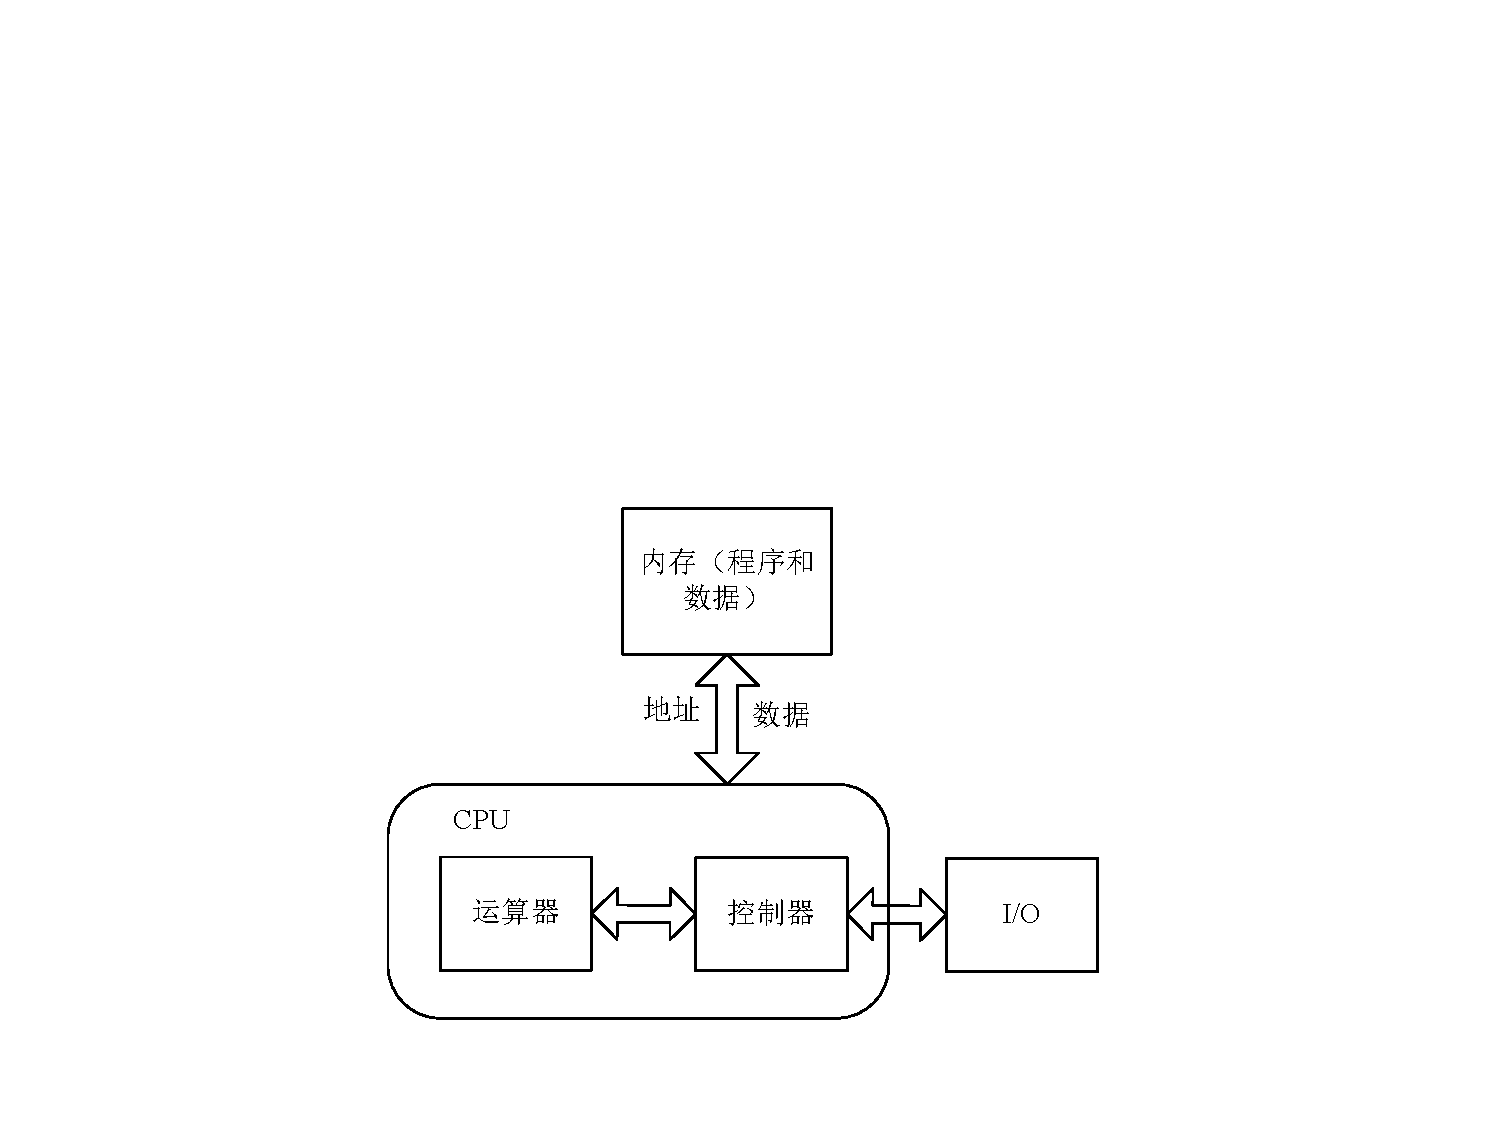
\includegraphics[width=6cm]{images/命令式(过程式)泛型.pdf}
    \vspace{-5em}
\end{wraptable}
用程序状态和改变程序状态的语句来描述计算

对冯·诺依曼式计算机的顺序执行机制的直接抽象

由过程完成复用

\subsubsection{面向对象的泛型}
\begin{itemize}
    \item 用封装了数据和操作的对象以及对象之间的消息传递描述计算
    \item 封装、继承、多态
\end{itemize}

\begin{figure}[H]
    \vspace{-0.5em}
	\centering
	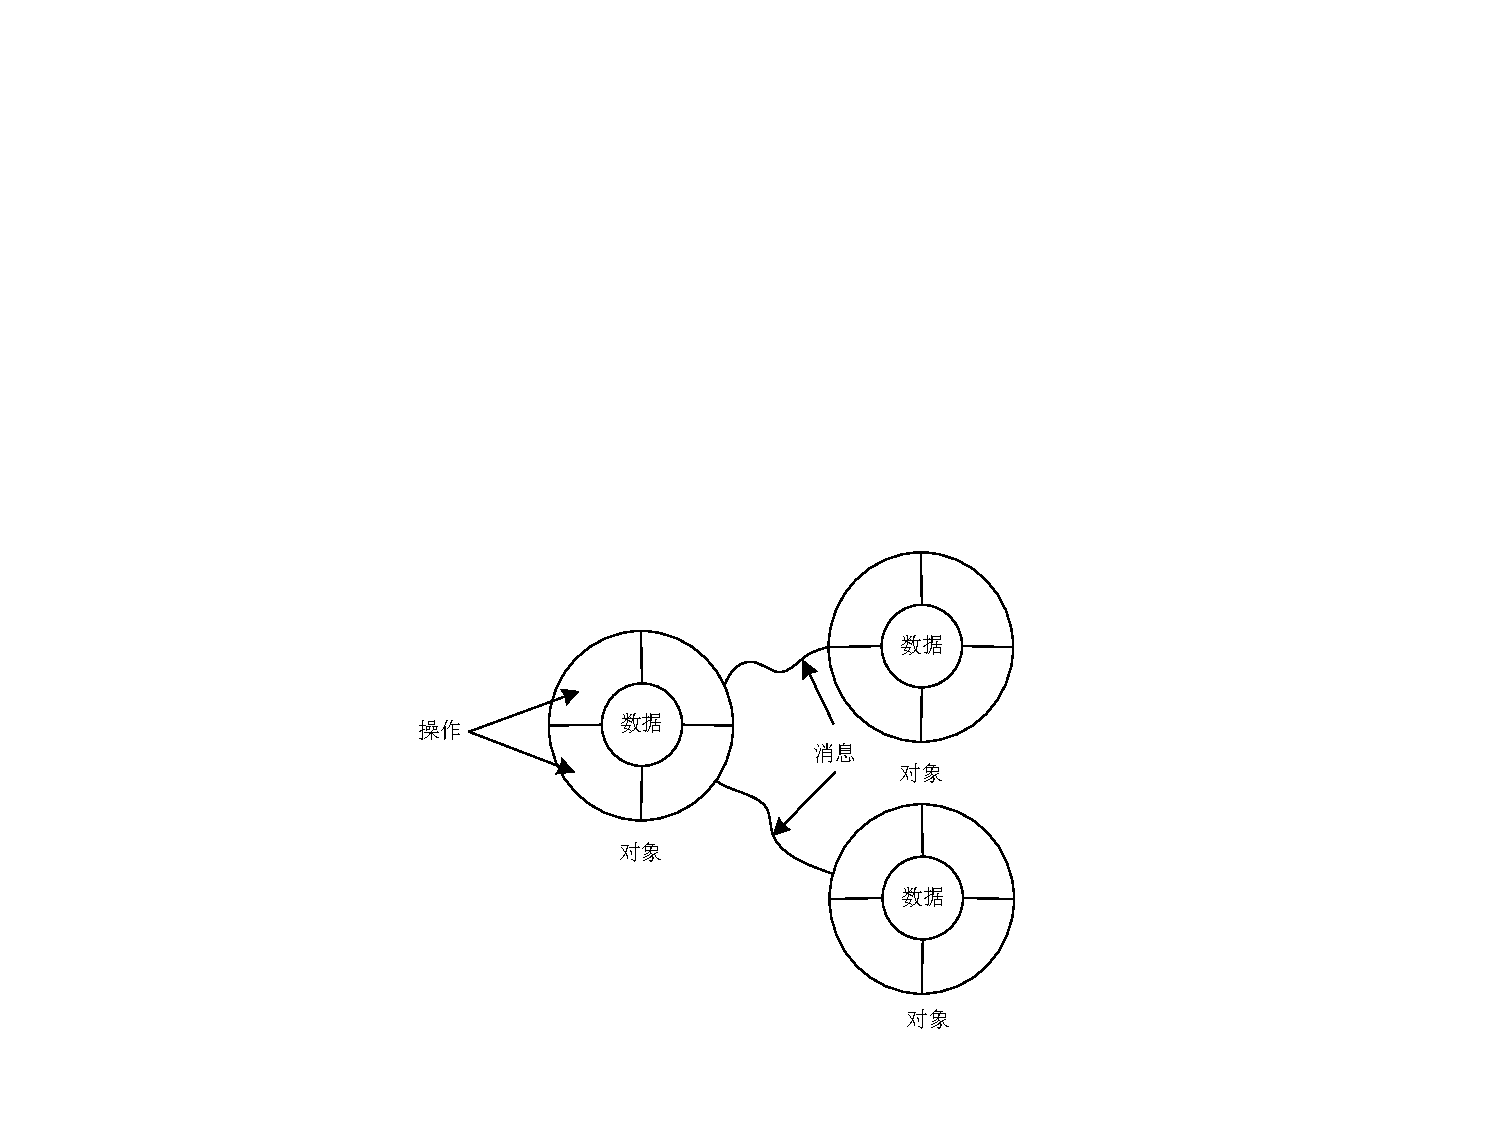
\includegraphics[width=0.45\textwidth]{images/面向对象的泛型.pdf}
    \vspace{-1em}
\end{figure}

\subsubsection{基于构件的泛型}
构件:模块化的、可部署、可替换的软件系统组成部分,它封装了内部的具体实现并对外提供统一接口。

以构建为基本单位进行分析和设计,整个软件的构造就被转换为:以构件的创建、构件的管理以及复用已有构件组装形成应用为基本活动。

\begin{spacing}{1}
    \begin{table}[H]
    \centering
    \begin{tabular}{|c|c|c|}
    \hline
                                                          & \textbf{基于构件}                                                                            & \textbf{面向对象}                                                                             \\ \hline
    抽象视角                                                  & \begin{tabular}[c]{@{}c@{}}构件是对客观世界的实体或者实体\\ 联合能提供的功能和服务的建模;\\ 仅仅关注实体的功能和服务\end{tabular} & \begin{tabular}[c]{@{}c@{}}对象是对客观世界基本实体的抽象,\\ 强调对实体的对应及对实体的建模;\\ 涉及实体的静态属性特征\end{tabular} \\ \hline
    \begin{tabular}[c]{@{}c@{}}可复用程度\\ 和复用机制\end{tabular} & 以组合的方式实现复用                                                                               & 以继承的方式实现复用                                                                                \\ \hline
    粒度不同                                                  & 大                                                                                        & 小                                                                                         \\ \hline
    \end{tabular}
\end{table}
\end{spacing}

\begin{figure}[H]
    \vspace{-0.5em}
	\centering
	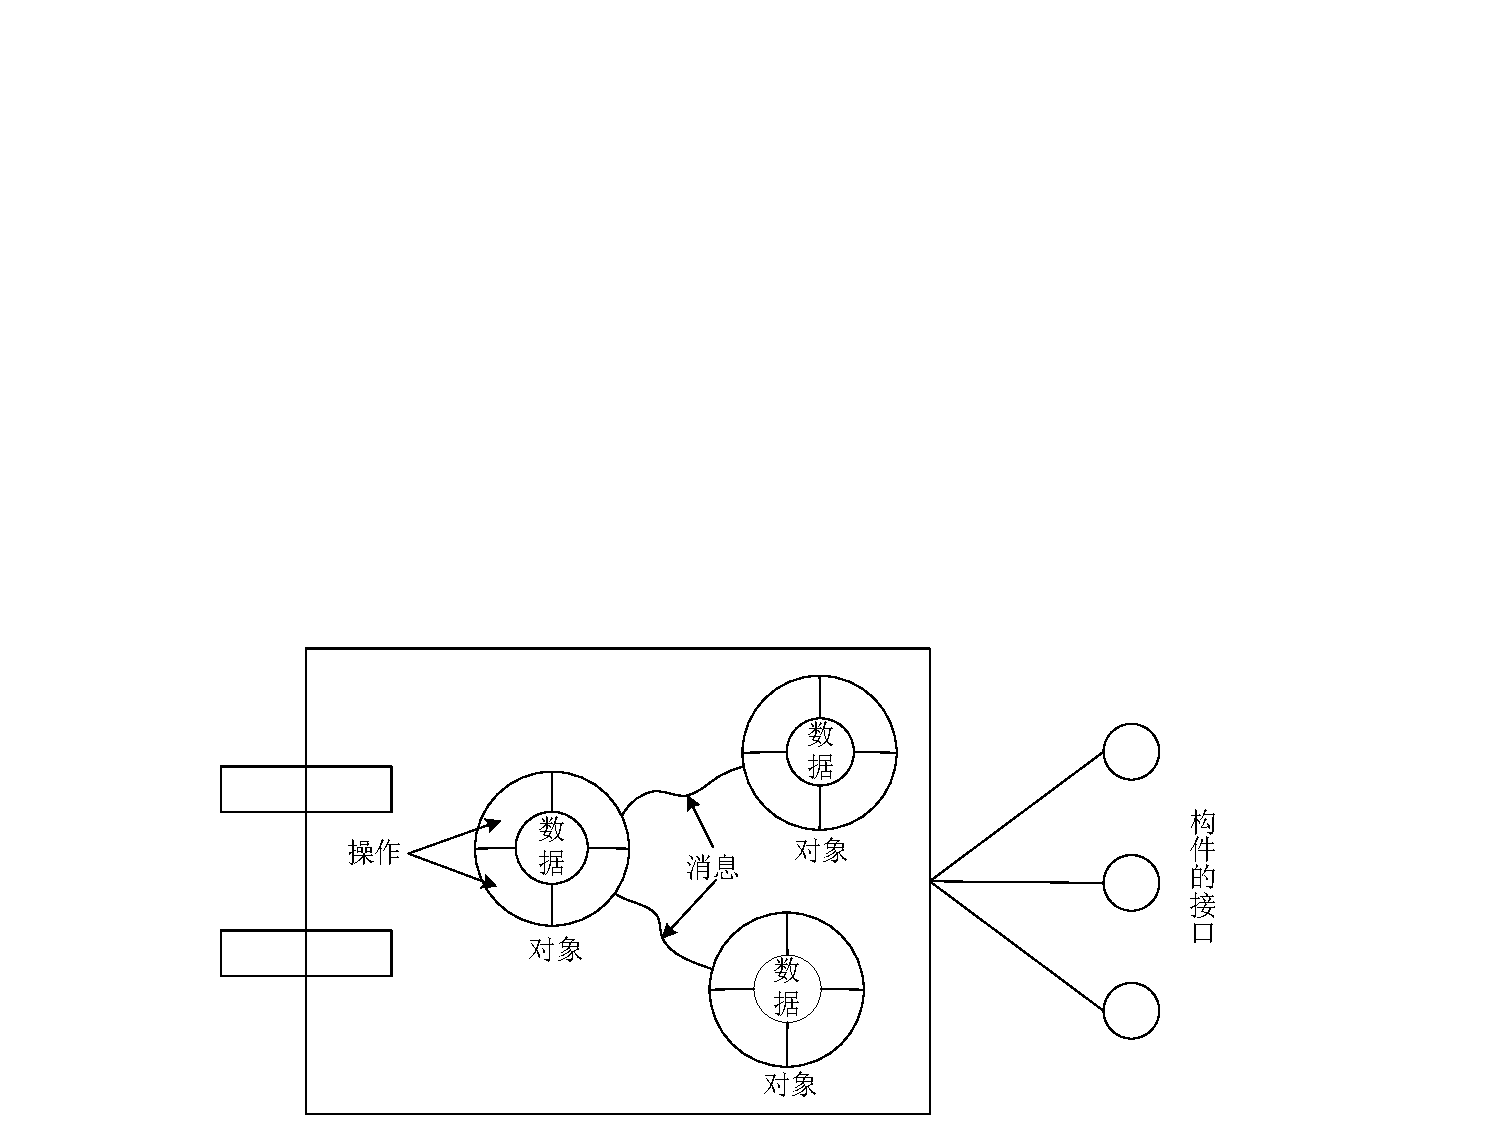
\includegraphics[width=0.65\textwidth]{images/基于构件与面向对象.pdf}
    \vspace{-1em}
\end{figure}

\subsubsection{面向服务的泛型}
\begin{itemize}
    \item 服务:是自治、开放、自描述、与实现无关的网络构件
    \begin{itemize}
        \item 自治:服务能够单独独立地完成一个任务(不依赖于其他构件,来完成它所需要完成的工作)
        \item 开放:对于构件而言,只要遵循了一般的协议或标准,当前服务的统一接口应该是跨公司、跨平台、全球范围之内可以相互调用的(进一步提升了它复用的可能性和范围)
        \item 自描述:服务应该自己能够描述自己完成的任务,而不应该有其他的附加手段去对于当前的服务来进行描述
        \item 与实现无关:只需提供统一接口,不用关心具体实现
    \end{itemize}
    \item 以服务的创建、服务的管理以及复用已有服务组装形成应用为基本活动
    \item 通过网络,使用标准方式互联
\end{itemize}

\begin{figure}[H]
    \vspace{-0.5em}
	\centering
	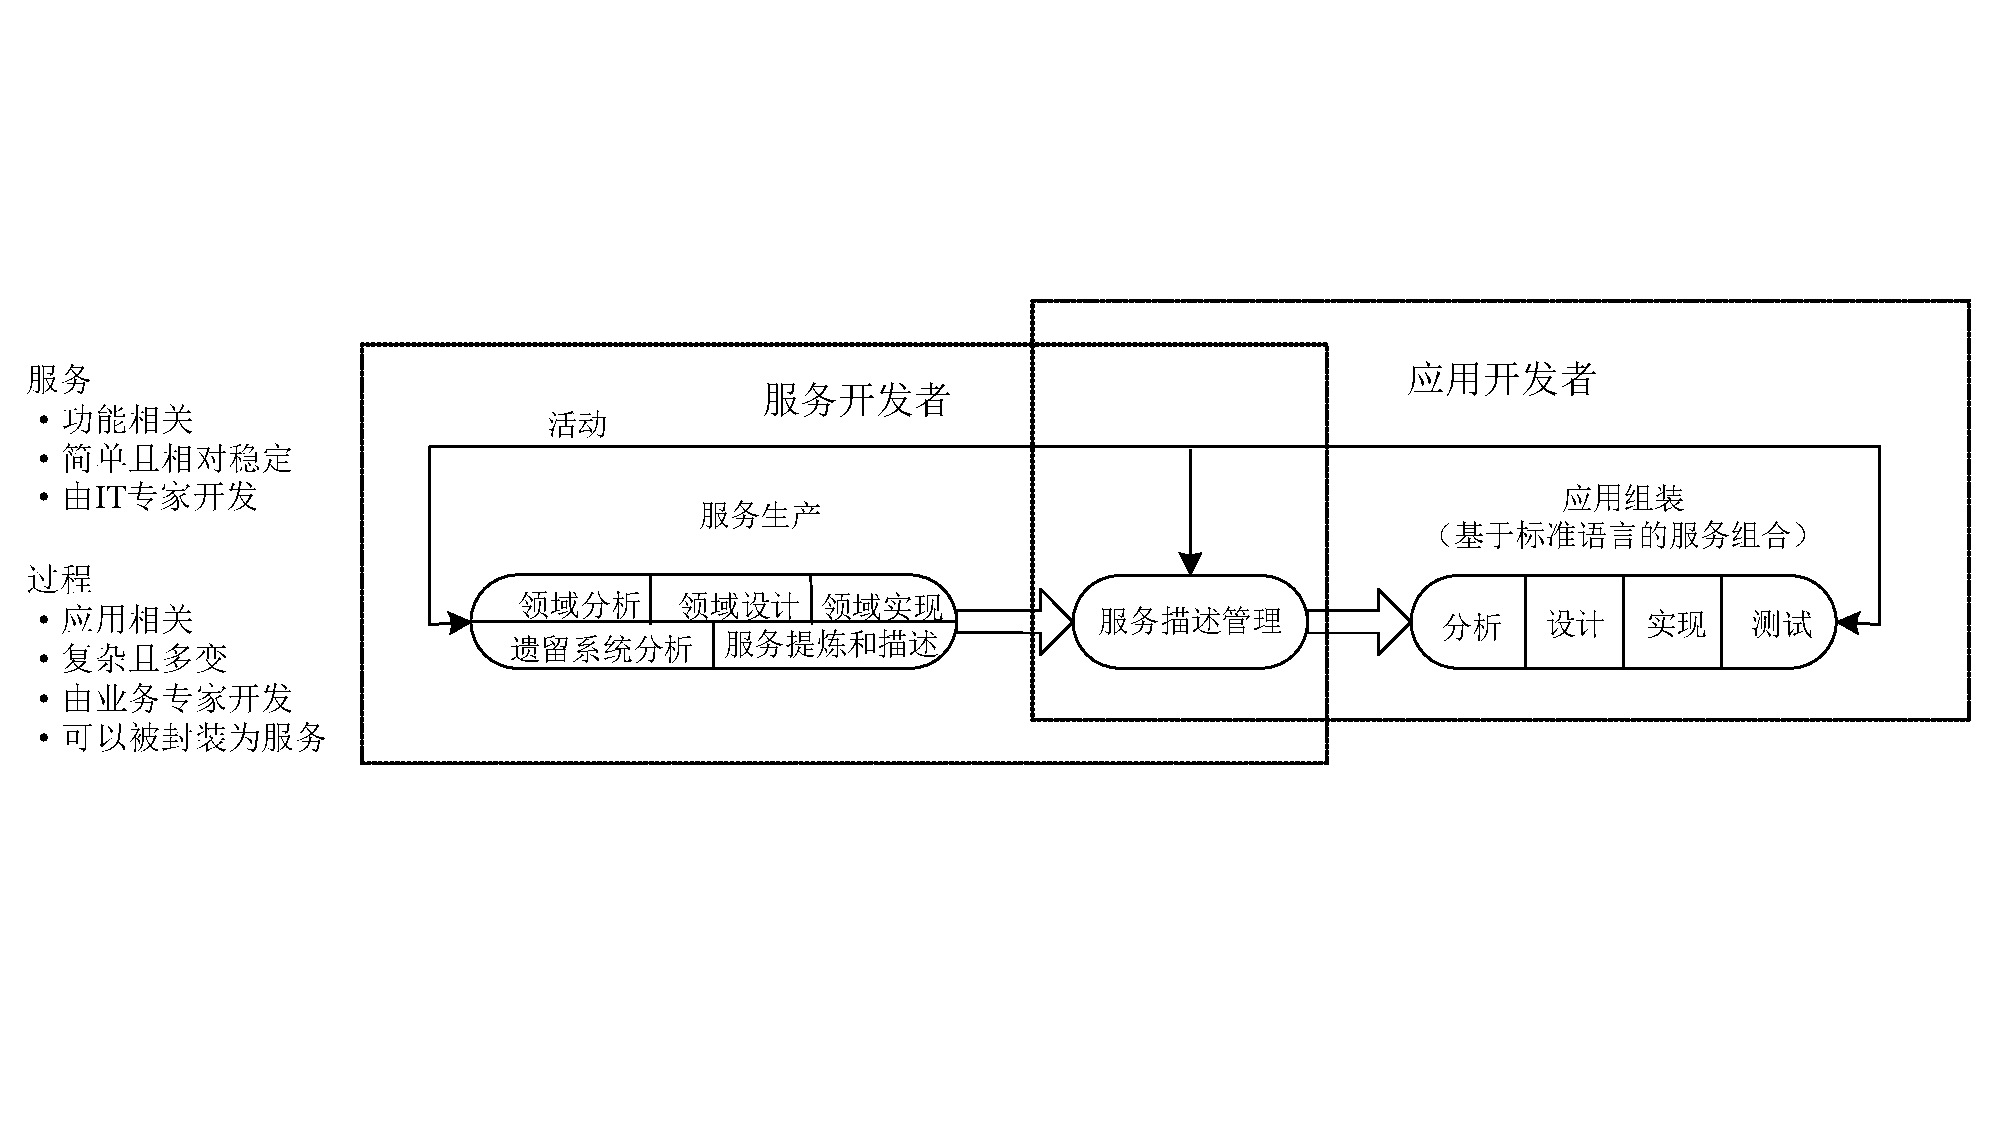
\includegraphics[width=\textwidth]{images/面向服务的泛型.pdf}
    \vspace{-1em}
\end{figure}


	\section{服务生态系统与面向服务的计算}

\subsection{服务生态系统}

面向服务的应用逻辑,遵循面向服务的设计原则,采用服务和服务组合加以实现。

\begin{figure}[H]
    \vspace{-0.5em}
	\centering
	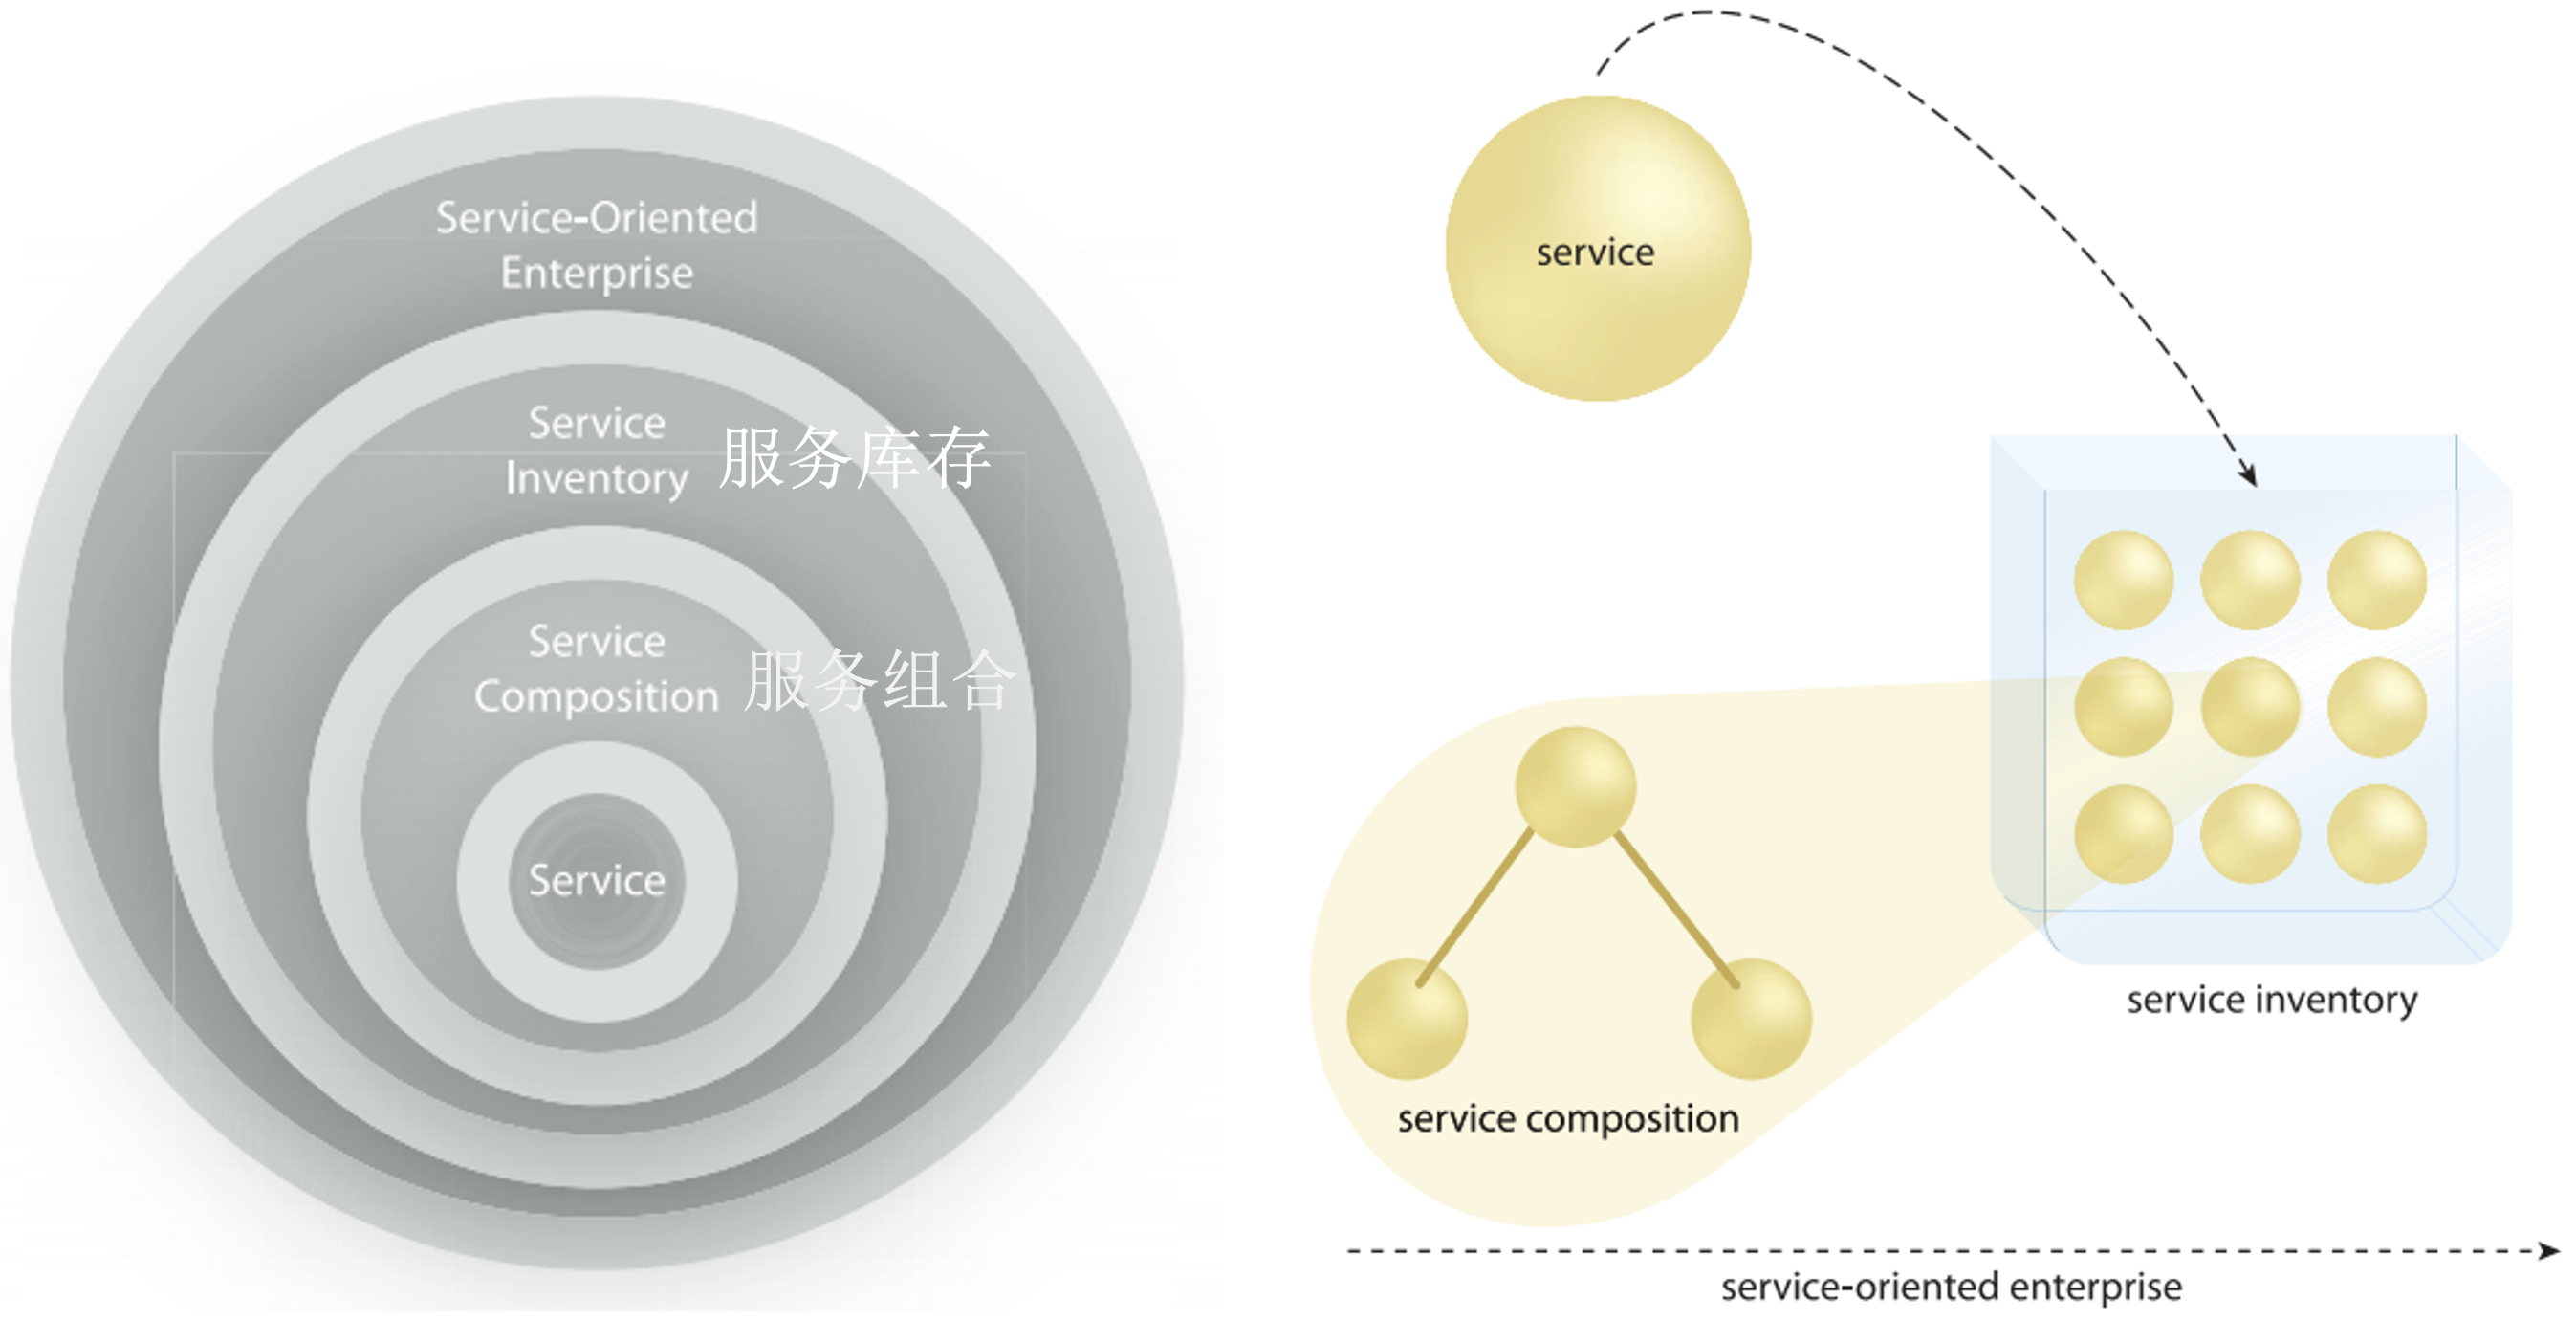
\includegraphics[width=0.8\textwidth]{images/面向服务的应用逻辑.png}
    \vspace{-1em}
\end{figure}

\subsubsection{服务组合}
服务组合由多个装配在一起的服务所构成,用以提供对业务任务或过程进行实现的功能。

由于面向服务倾向于将服务打造为无关的企业资源,一个服务可能被多个消费者程序所调用,它们能在不同的服务组合中组合同一个服务。


\subsubsection{服务库存}
服务库存,是在组织或组织的合理部分边界内一组独立标准化并治理的完备服务。

\begin{figure}[H]
    \vspace{-0.5em}
	\centering
	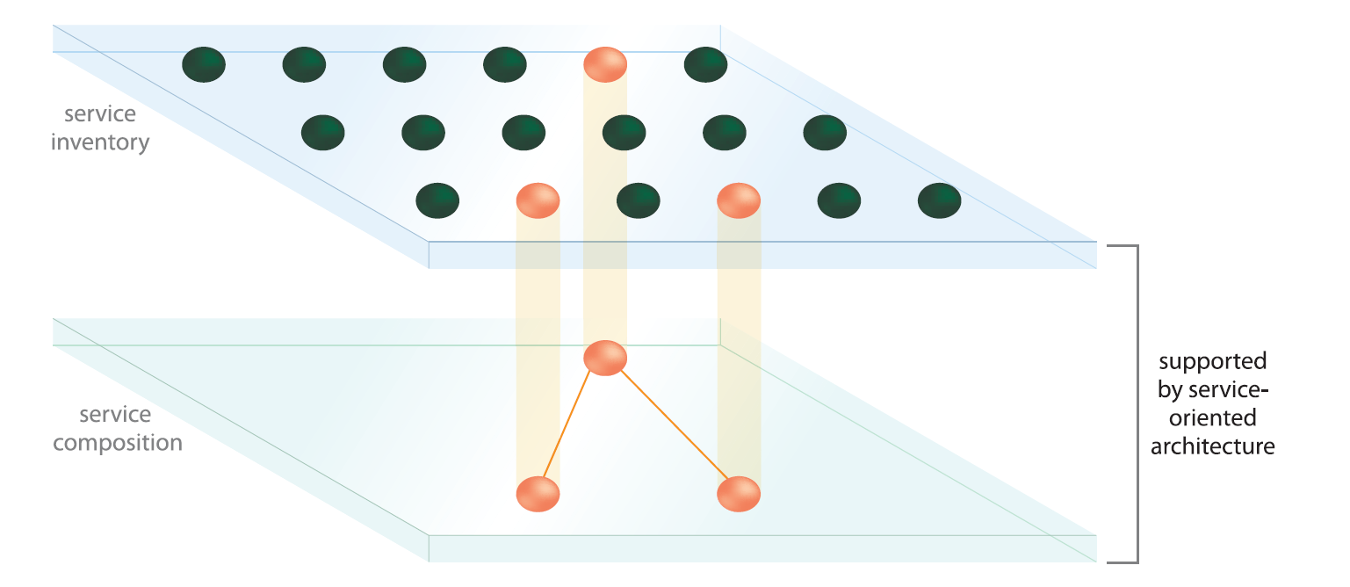
\includegraphics[width=0.8\textwidth]{images/服务库存与服务组合.png}
    \vspace{-1em}
\end{figure}

服务库存可以按照服务模型进行分层:
\begin{itemize}
    \item 应用服务层:紧密和实现相关的较小功能单元抽象出来的服务。
    \item 业务服务层:直接满足调用者、消费者需求的服务
    \vspace{-0.8em}
    \begin{multicols}{2}
        \begin{itemize}
            \item 以任务为中心的业务服务(任务服务)
            \item 以实体为中心的业务服务(实体服务)
        \end{itemize}
    \end{multicols}
    \vspace{-1em}
    \item 编排服务层:(可选的服务层)服务组合的一种实现,一般由领域专家实现,使用平台中立语言(文本化的标记语言,一般为 XML)来描述服务组合的业务逻辑。
\end{itemize}

\begin{figure}[H]
    \vspace{-0.5em}
	\centering
	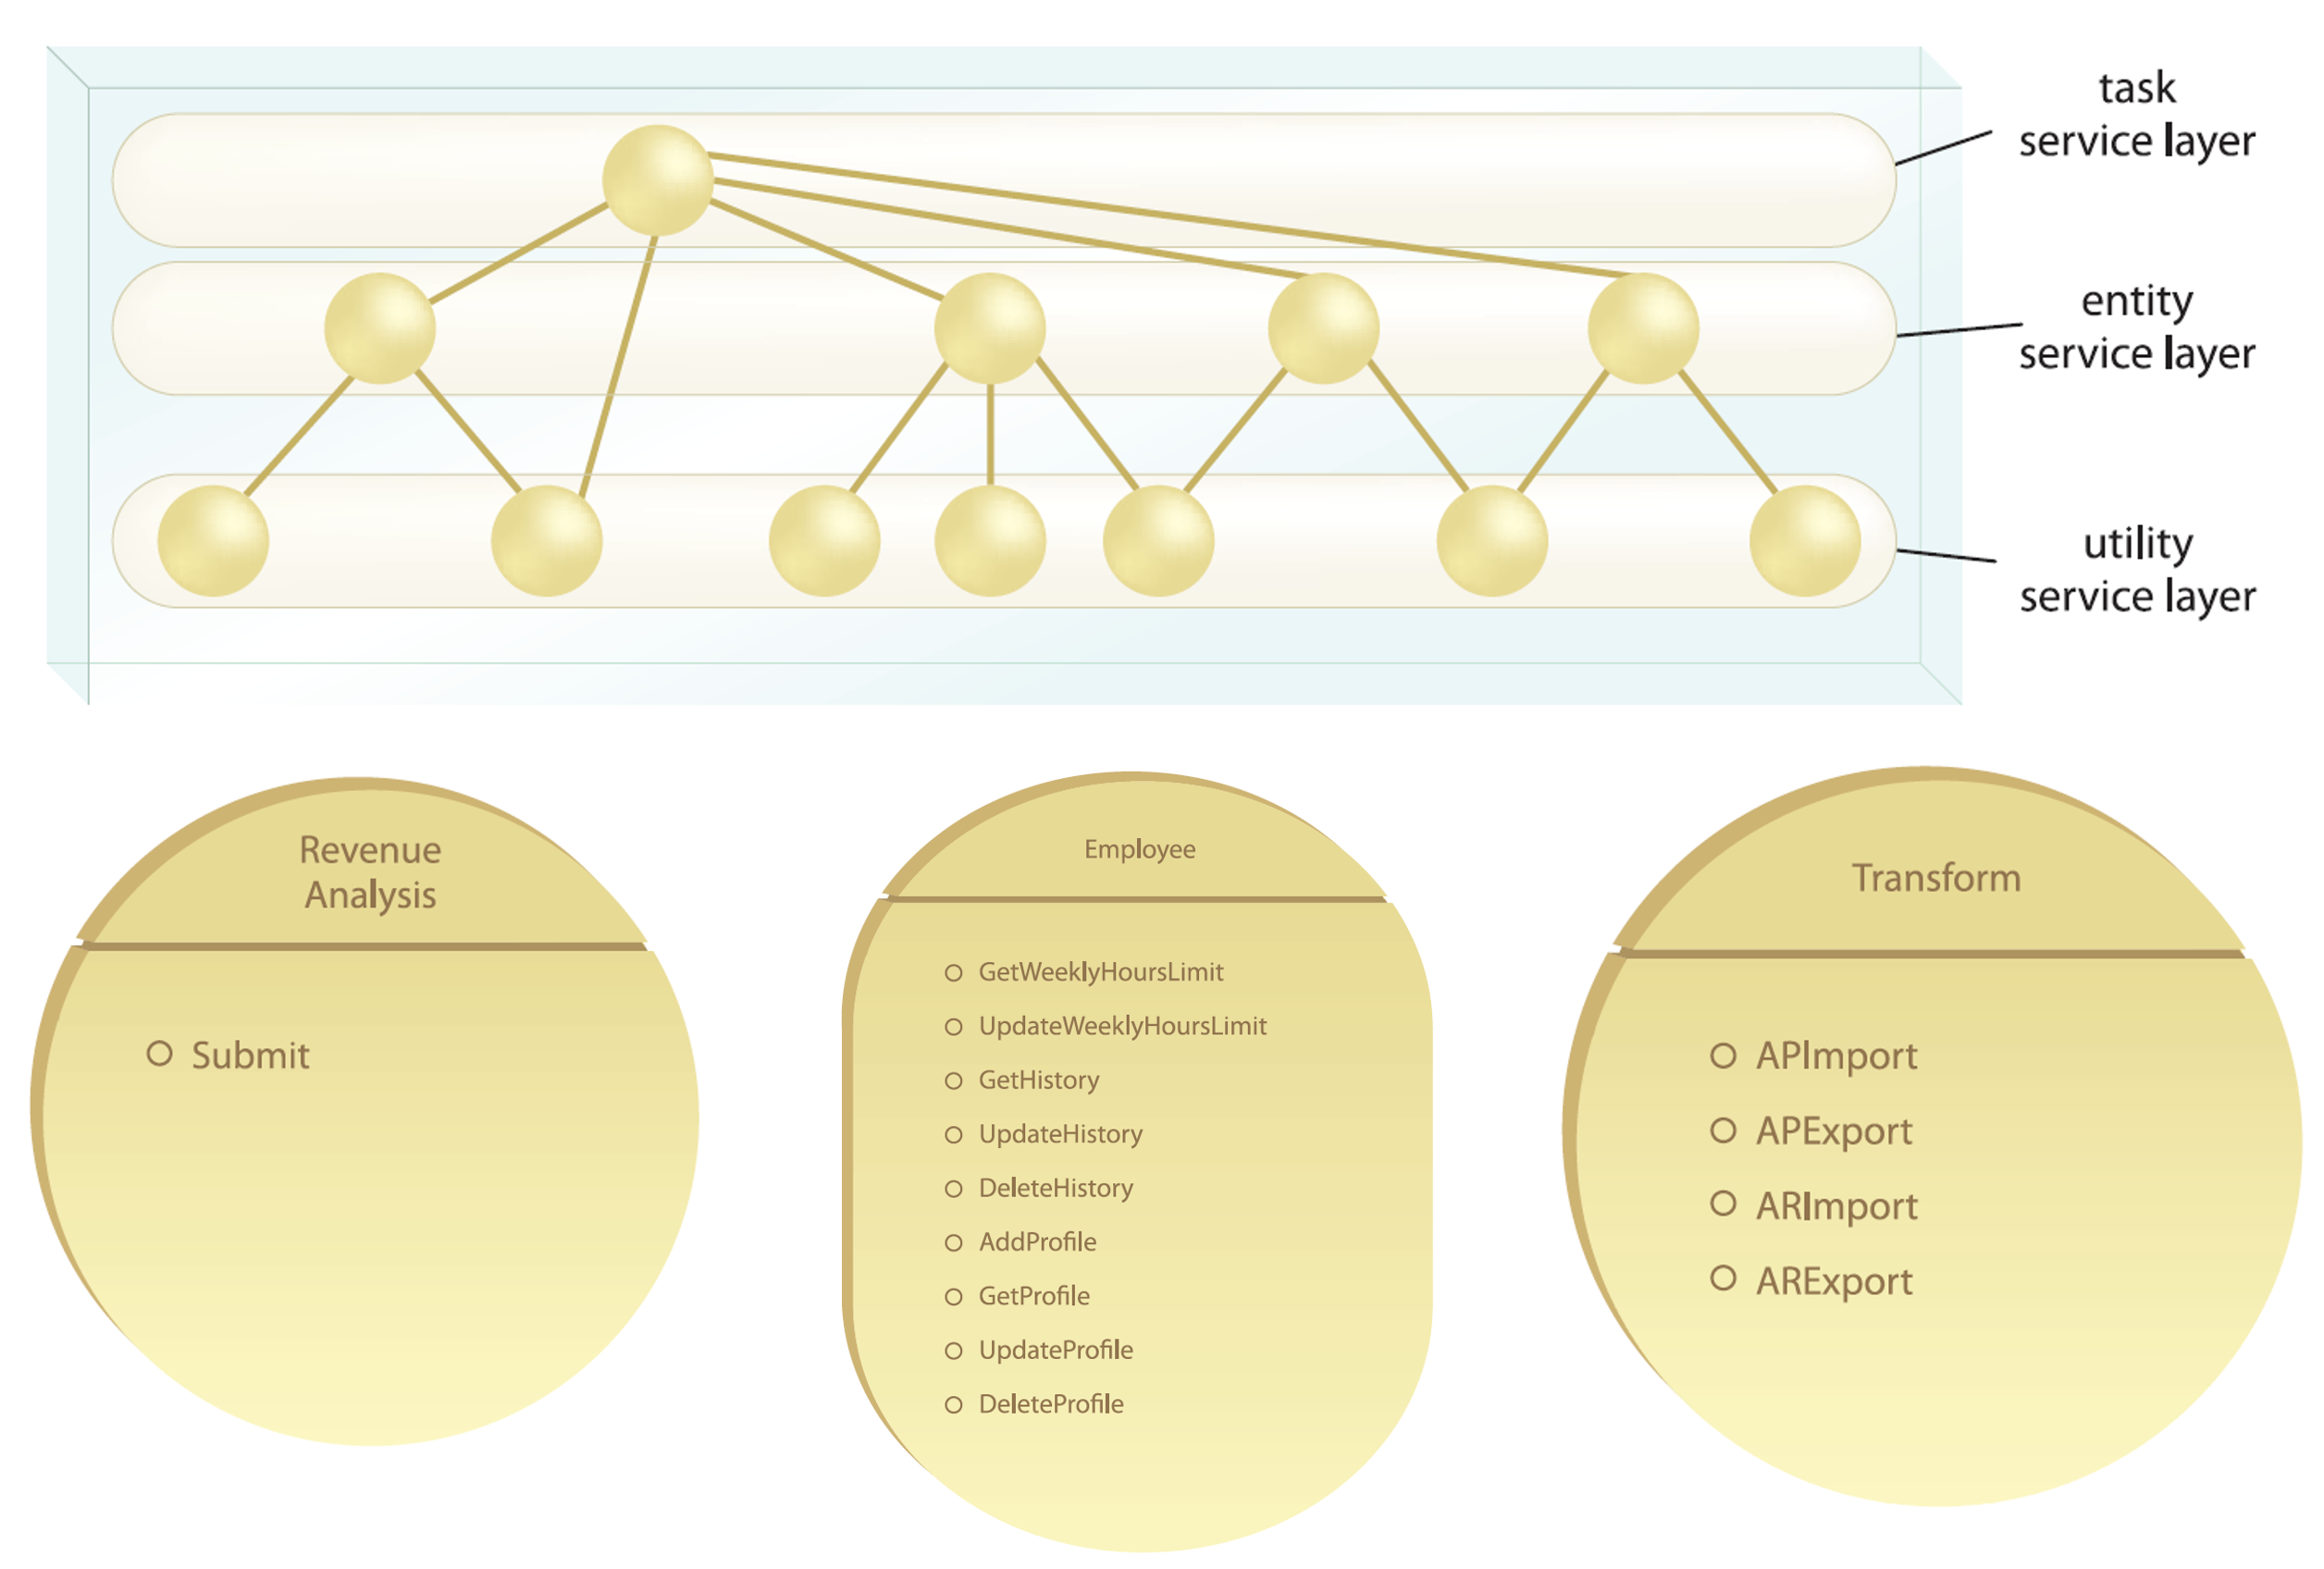
\includegraphics[width=0.7\textwidth]{images/服务模型.png}
    \vspace{-1em}
\end{figure}

在构建前,服务库存的蓝图就已设计完毕了。

服务库存的演化阶段:
\begin{itemize}
    \item 初始服务交付项目(按需开发):服务是中立的,独立于当前软件系统,独立于调用它的服务系统或应用。
    \item 混合应用和成长中的服务库存:服务的数量持续增长,服务组合的可能性也持续增长,但是服务库存仍然尚未完成。
    \item 服务库存基本构建完毕:服务库存的演化基本完成。随着服务库存的增长,潜在的服务组合的复杂度也随之提升。
\end{itemize}


\subsubsection{服务生态系统}
当服务库存按照面向服务的方式进行良好的规划和设计、经过长时间演化、已经基本完备;该组织的服务系统均已合理地转向面向服务的实现,那么该组织内的服务生态系统就被构建起来了。

包含分析、设计、实现、治理、演化等……
\begin{itemize}
    \item 治理:由于共享计算,通过网络以统一的接口调用服务,故需要提供相应的计算资源,来尽量满足所有人的需求。
\end{itemize}
\vspace{-0.8em}
\begin{multicols}{2}
    \begin{itemize}
        \item 兼容性演化:接口不变,后台实现发生变化
        \item 非兼容性演化:接口也需要改变
    \end{itemize}
\end{multicols}
\vspace{-1em}

从消费者角度出发:
\begin{itemize}
    \item 可以被同时、独立调用的,用于满足消费者需求的服务被称为垂直服务(消费者直接调用的服务)。
    \item 垂直服务可以由多个可重用的跨领域的公共服务所构成,这些服务被称为水平服务(不直接被消费者调用的服务)。
    \item 垂直服务和水平服务不是互斥的;二者的区别的唯一标准就在于在某一特定场景下,是否被消费者直接调用。当水平服务被消费者直接调用时,就是也是作为垂直服务。
\end{itemize}


\subsection{服务计算}

\subsubsection{服务计算的定义}
服务计算也叫面向服务的计算(SOC)
\begin{itemize}
    \item 从泛型角度出发:面向服务的计算是一种新型计算泛型。该泛型以服务作为基本概念,以支持快速和低成本开发,和异构环境中分布式应用的灵活组合。
    \item 从软件架构角度出发:面向服务的计算是一组使用面向服务的架构(SOA)来表达计算的概念、原理和方法。在面向服务的架构中,使用带有标准接口的独立构件服务来构造软件应用。
    \item  从服务角度出发:为了在业务服务和IT服务之间建立连接,并进一步改进业务服务,面向服务的计算涵盖了运用计算和信息技术建模、创建、操作和管理业务服务的科学和技术。
    \item 从软件工程的角度出发:面向服务的计算盖了使用服务作为基本抽象元素,采用工程化方法,对服务系统进行分析、设计、开发、测试、部署、管理等活动所涉及的理论、技术和方法。
\end{itemize}

\subsubsection{面向服务与面向服务的目标}
\begin{figure}[H]
    \vspace{-0.5em}
	\centering
	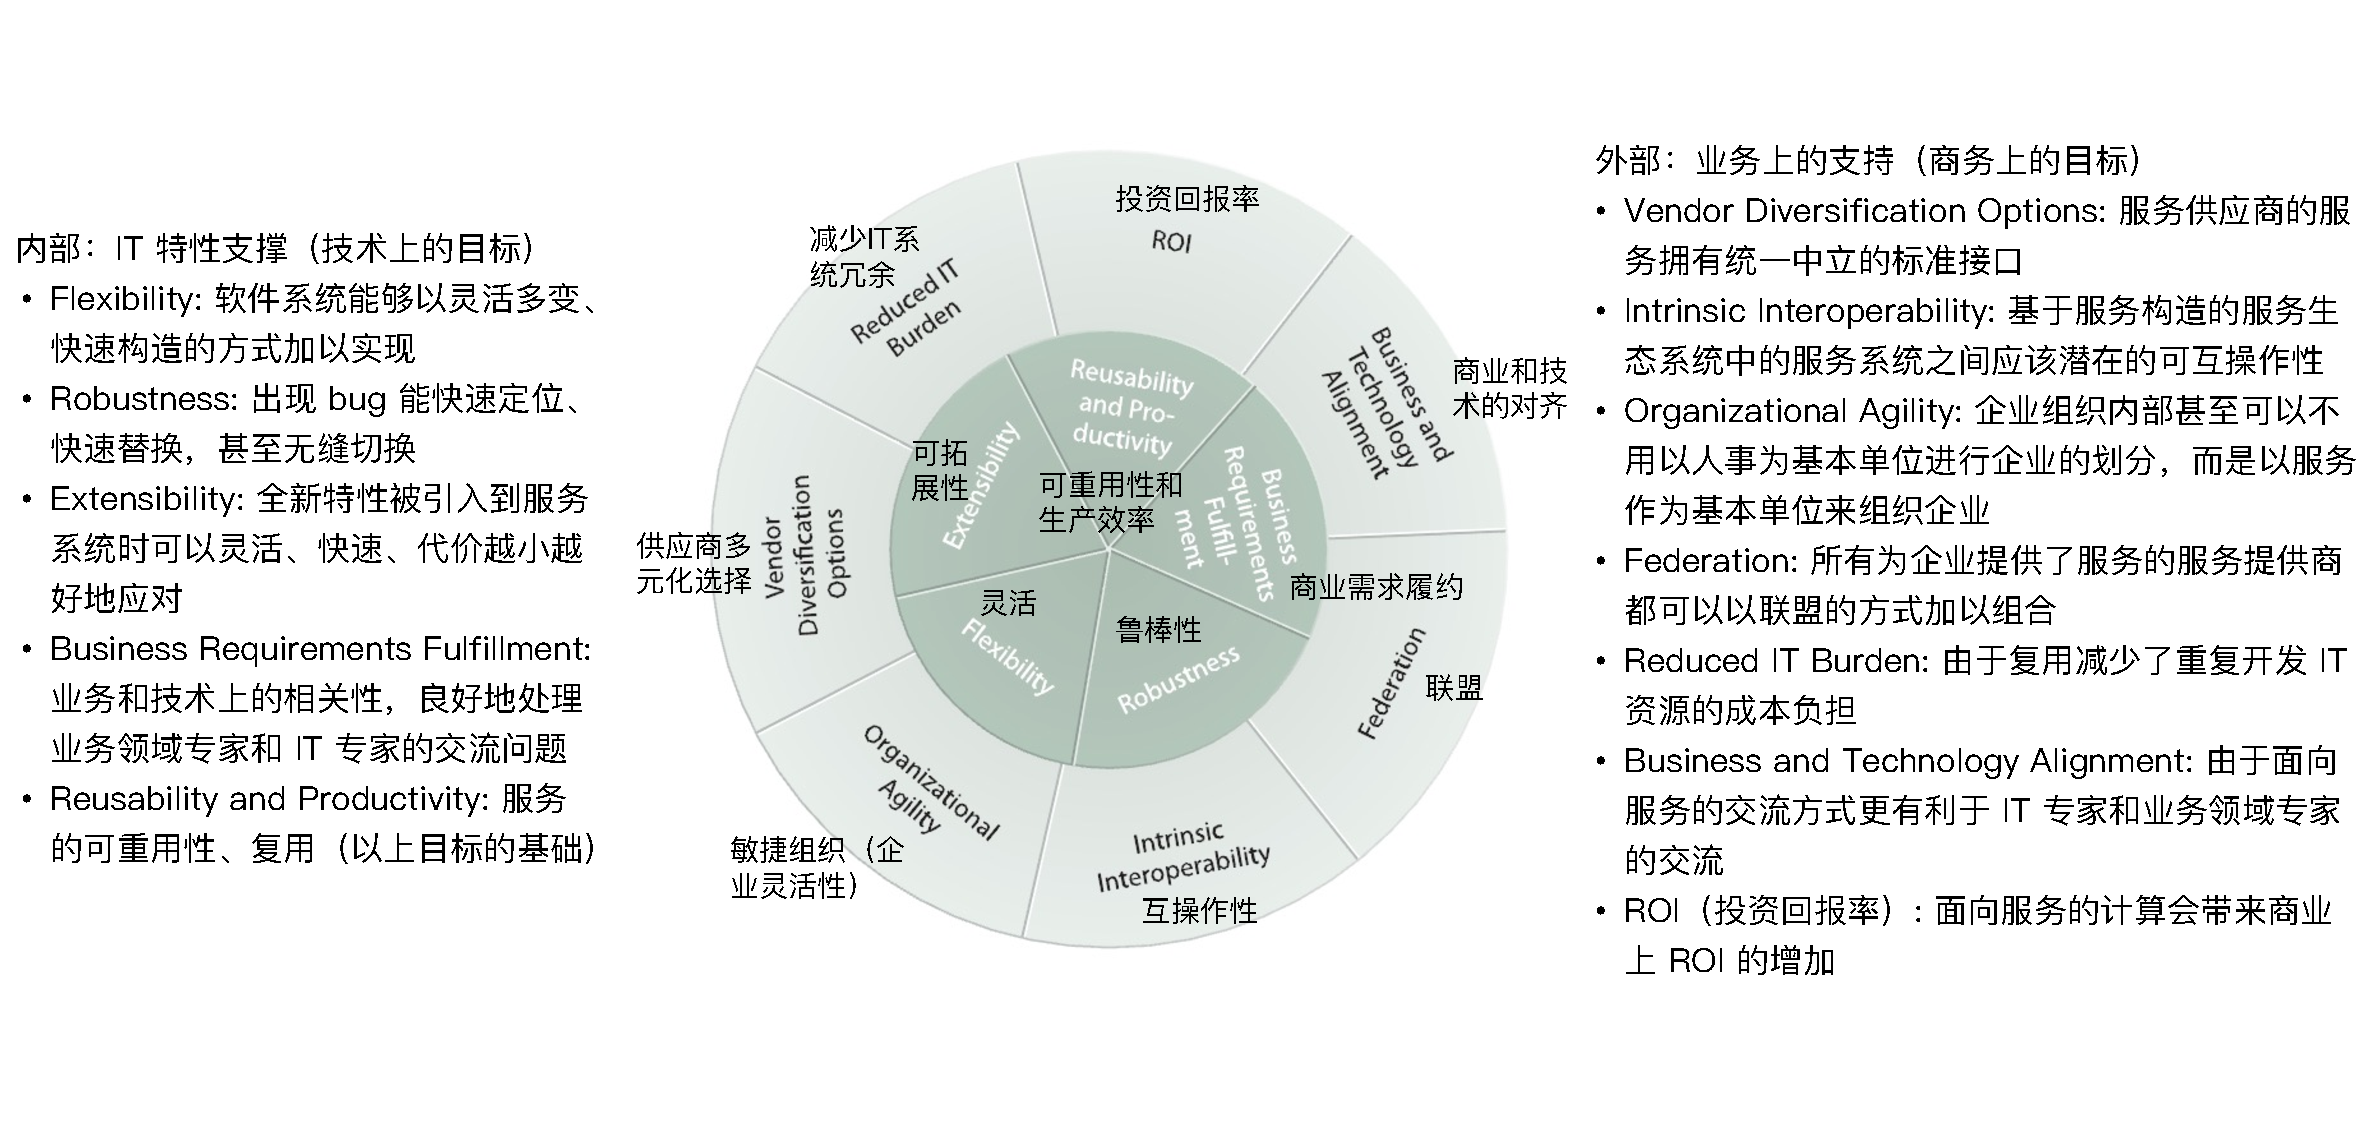
\includegraphics[width=\textwidth]{images/面向服务的目标.pdf}
    \vspace{-2em}
\end{figure}


\subsection{面向服务与面向对象}

\subsubsection{面向服务与面向对象的对比}
\vspace{-0.5em}
\begin{spacing}{1.2}
    \centering
    \begin{longtable}{|m{1.8cm}<{\centering}|m{6.5cm}|m{6.5cm}|}
		\hline
    \textbf{特点} & \multicolumn{1}{c|}{\textbf{面向对象的计算}}                   & \multicolumn{1}{c|}{\textbf{面向服务计算}}                                                          \\ \hline
    方法论         & 通过定义紧耦合的类来进行应用开发;应用架构为基于继承关系的层次式架构;从构造函数——通过类或模型——到系统设计 & 通过定义松耦合的服务来进行应用开发,并将服务组装成可执行的应用;从系统模型到服务模块,从服务抽象定义到服务实现绑定;通过搜索获得可用的服务实现                       \\ \hline
    抽象和协作层次     & 往往由一个团队来负责应用的开发,并负责整个生命周期;开发者必须了解应用领域知识和编程              & 开发任务由三个独立方承担:应用程序开发者,服务提供方和服务代理;其中,应用程序开发者需要了解应用逻辑,但不需要了解具体的服务是如何实现的;服务提供者需要编程能力,但不必了解使用服务的应用 \\ \hline
    代码共享和复用     & 代码复用通过类成员的继承和库函数加以实现。其中库函数在编译时引入,且往往是平台相关的              & 代码在服务层次复用。服务使用标准的结构,并发布在Internet库中。服务是平台无关的,且能够被查找并远程调用。服务代理支持系统的服务共享                         \\ \hline
    动态绑定和重新组合   & 在运行时将名称和方法进行关联。方法必须在应用部署前链接到可执行的代码                      & 在运行时将服务调用和服务进行绑定。可以在应用部署后,再进行服务选定。这一特色使得应用可以在运行时重组                                            \\ \hline
    重组          & 多在设计时决定导入的组件                                            & 可以动态改变应用系统中服务的组合关系,以及服务定义与服务实现之间的绑定关系,即实现动态地添加、修改、删除各个服务节点                                    \\ \hline
    组件通讯和接口     & 与平台和语言有关,例如C++程序难以直接和Java程序通信                           & 与平台和语言无关。组件间通过标准协议通信,如XML,WSDL和SOAP                                                           \\ \hline
    系统维护        & 用户需要时常升级软件,且在执行升级时,应用必须停止                               & 通过互联网升级系统,因为服务多运行在远程服务器上,用户通过互联网进行访问。维护对用户透明                                                  \\ \hline
    可靠性         & 在设计时决定可靠性的方法                                            & 对于服务提供者,每个服务相对简单,更加可靠。对于应用程序存在多个满足同一需求的服务,可用过将故障服务的节点断开并重新绑定到备选服务节点上,获得不间断的应用系统               \\ \hline
    软件拥有        & 软件作为产品销售,为用户所拥有                                         & 软件存在并执行于独立的服务提供商的设备上,用户按照每次对服务使用付费,而不是按照软件产品付费                                                \\ \hline
    \end{longtable}
	\end{spacing}
\vspace{-0.5em}


从设计角度和实现角度来看
\vspace{-0.5em}
\begin{spacing}{1.2}
    \centering
    \begin{longtable}{|m{1.2cm}<{\centering}|m{6.7cm}|m{6.7cm}|}
        \hline
\textbf{特点} & \multicolumn{1}{c|}{\textbf{面向对象的计算}} & \multicolumn{1}{c|}{\textbf{面向服务计算}} \\ \hline
耦合          & 提倡重用和松耦合,但是预先定义的类依赖导致更多的对象紧密绑定        & 服务的松耦合由功能和服务合约给定                     \\ \hline
粒度          & 为支持不同规模的任务,支持细粒度接口(API)               & 鼓励粗粒度的接口(服务描述),通讯消息中包含尽可能多的任务相关信息    \\ \hline
作用域         & 对象作用域更小,更有针对性(往往基于一个软件系统)             & 服务作用域显著不同(往往基于一个服务生态系统)              \\ \hline
前瞻性         & 鼓励处理逻辑与数据的绑定从而产生对象                    & 鼓励创建活动无关的、由消息驱动的服务                  \\ \hline
状态性         & 数据和逻辑的绑定,导致带状态的对象                     & 服务尽可能保持无状态性                          \\ \hline
组合          & 在支持对象组合的同时也支持对象的继承,从而导致紧耦合            & 支持松散耦合服务的组合                          \\ \hline
    \end{longtable}
\end{spacing}
\vspace{-0.5em}

\subsubsection{对象/类/接口与服务合约}
\begin{figure}[H]
    \vspace{-0.5em}
	\centering
	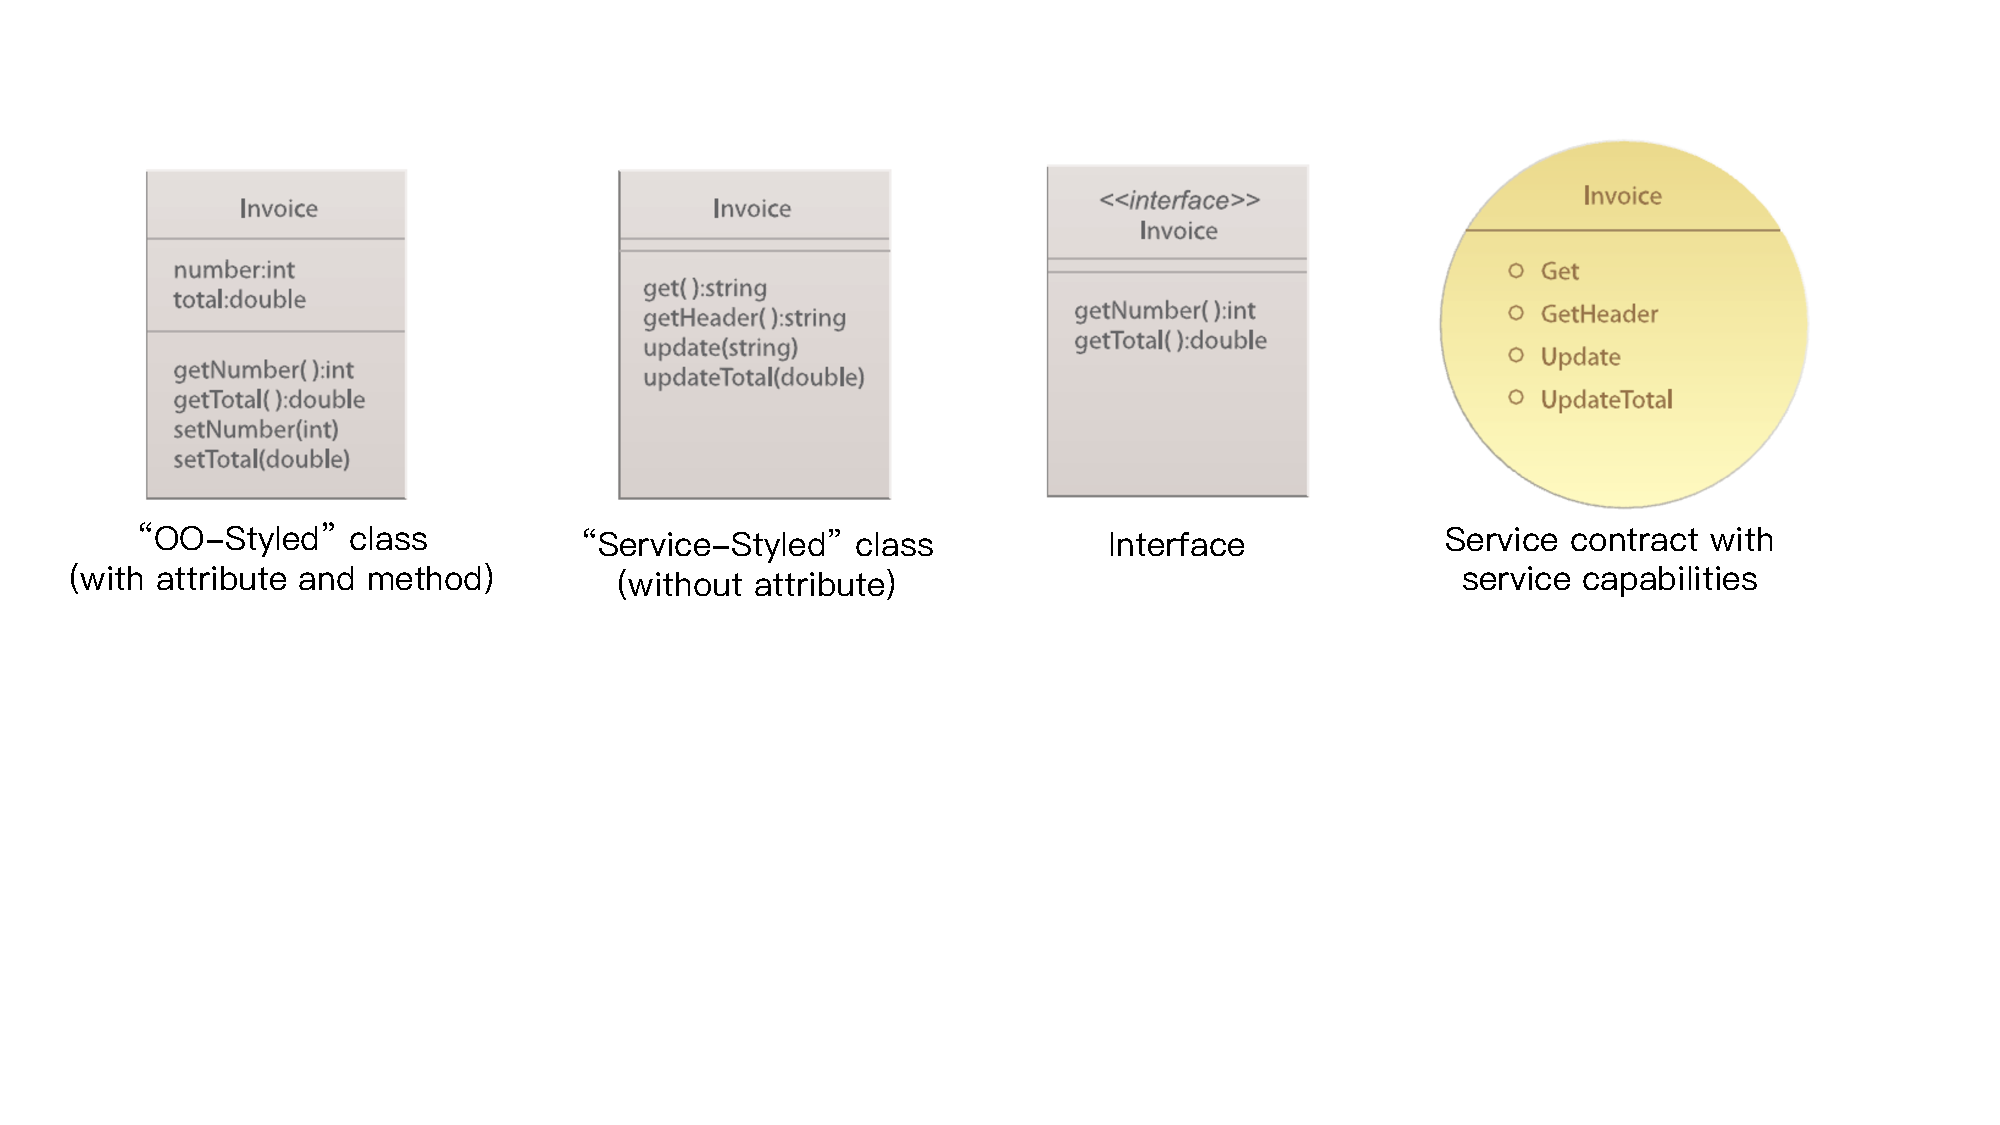
\includegraphics[width=0.8\textwidth]{images/对象、类、接口与服务合约.pdf}
    \vspace{-1em}
\end{figure}

\subsubsection{面向对象设计原则之于面向服务}
面向对象的基本原则
\vspace{-0.8em}
\begin{multicols}{4}
    \begin{spacing}{1.1}
        \begin{itemize}
            \item 封装
            \item 继承
            \item 泛化和特化
            \item 抽象
            \item 多态
            \item 开闭原则
            \item 别重复你自己
            \item 单一职责原则
            \item 委托
            \item 关联
            \item 组合
            \item 聚合
        \end{itemize}
    \end{spacing}
\end{multicols}
\vspace{-1em}

\begin{figure}[H]
	\setcounter{subfigure}{0}
	\centering
	\vspace{-0.5em}	
	\subfloat[封装]{
	\begin{minipage}[t]{0.47\linewidth}
	\centering
	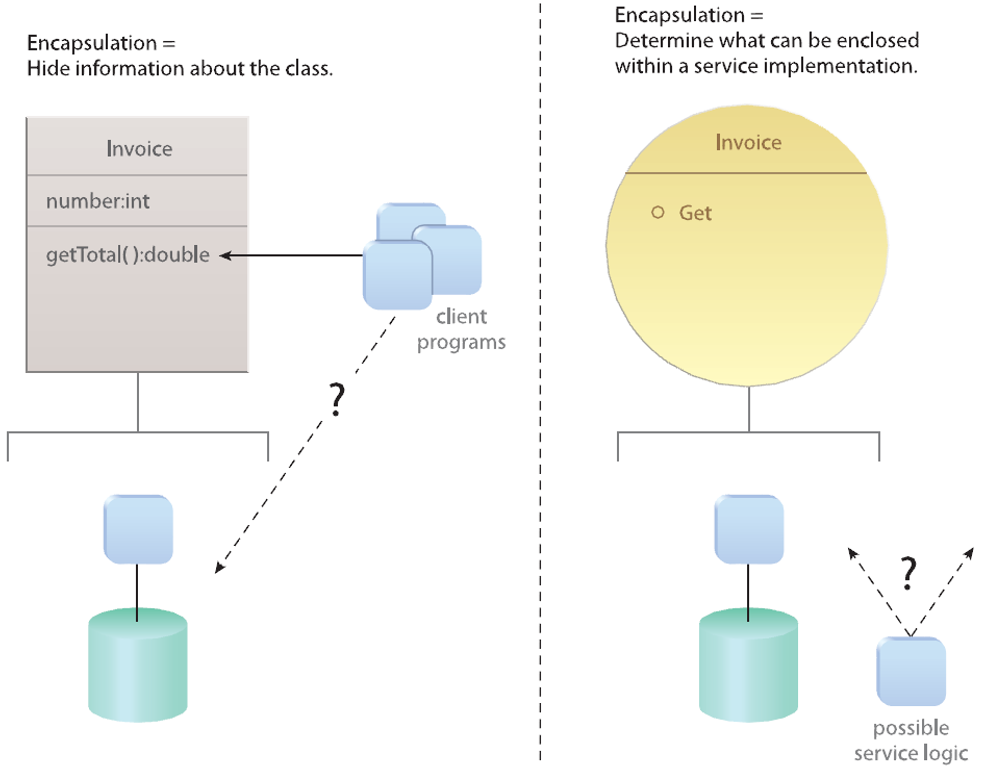
\includegraphics[width=0.97\linewidth]{images/封装.png}
	\end{minipage}
	}
    \hfill
	\subfloat[泛化和特化]{
	\begin{minipage}[t]{0.44\linewidth}
	\centering
	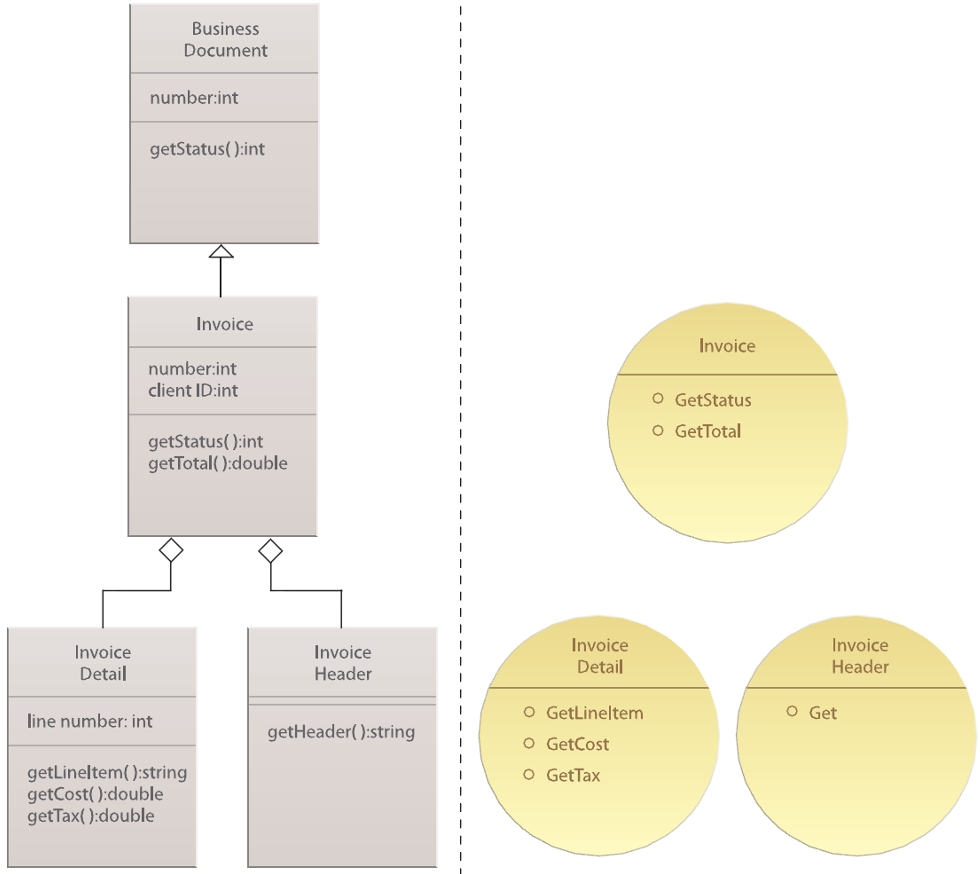
\includegraphics[width=0.97\linewidth]{images/泛化和特化.png}
	\end{minipage}
	}

    \subfloat[抽象]{
	\begin{minipage}[t]{0.31\linewidth}
	\centering
	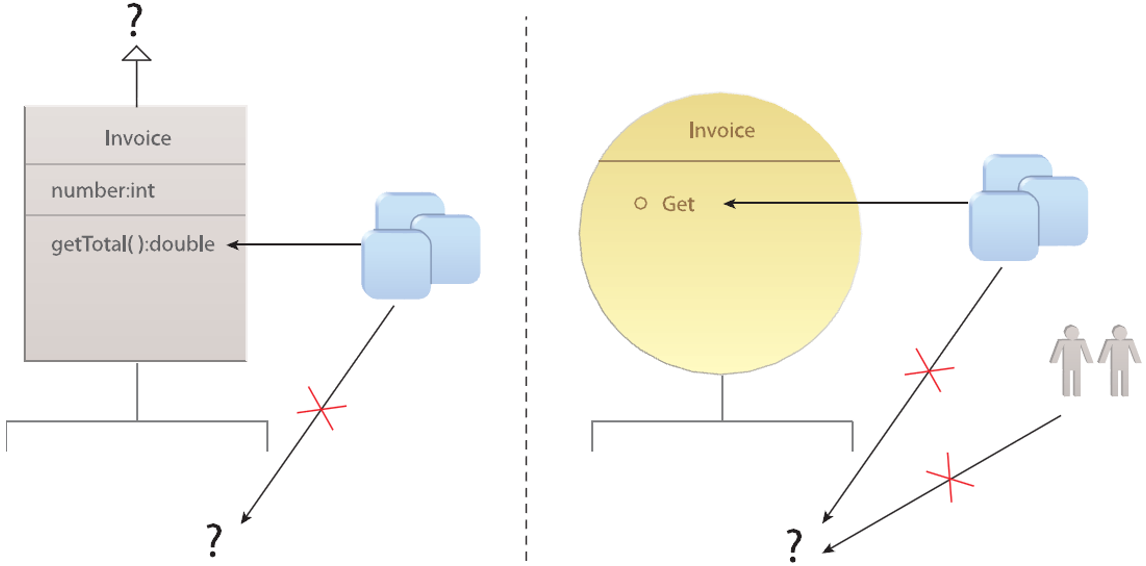
\includegraphics[width=0.97\linewidth]{images/抽象.png}
	\end{minipage}
	}
	\subfloat[继承]{
	\begin{minipage}[t]{0.31\linewidth}
	\centering
	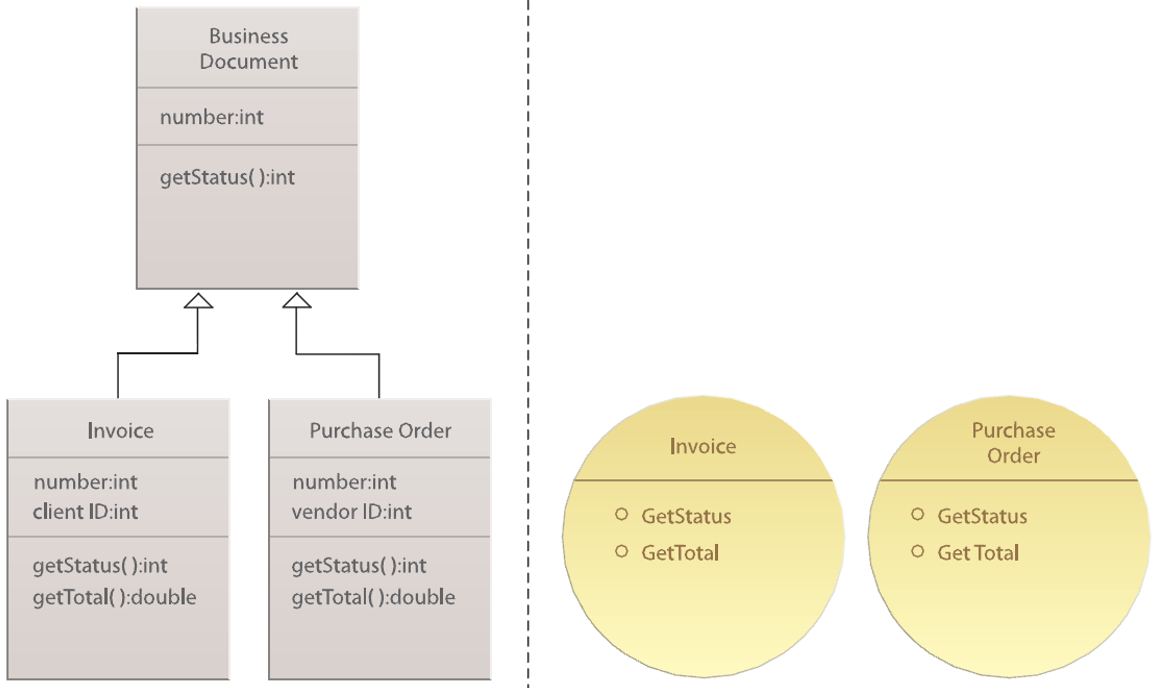
\includegraphics[width=0.97\linewidth]{images/继承.png}
	\end{minipage}
	}
    \subfloat[多态]{
	\begin{minipage}[t]{0.31\linewidth}
	\centering
	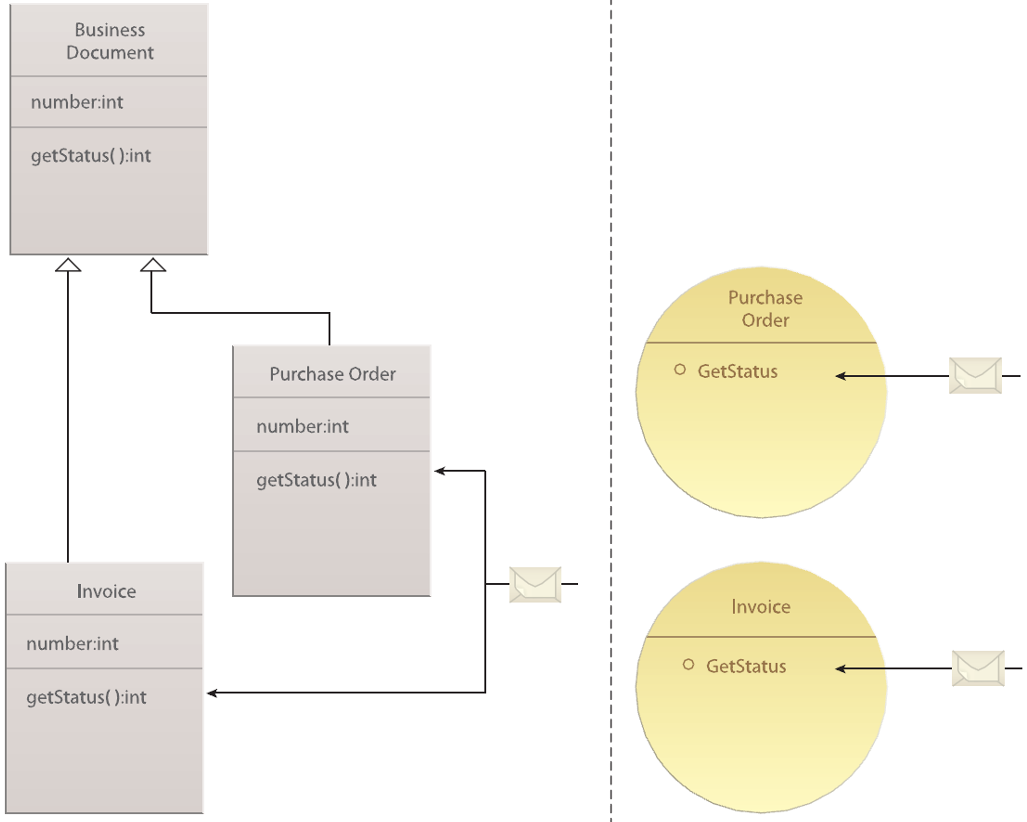
\includegraphics[width=0.97\linewidth]{images/多态.png}
	\end{minipage}
	}
    
	\subfloat[开闭原则]{
	\begin{minipage}[t]{0.53\linewidth}
	\centering
	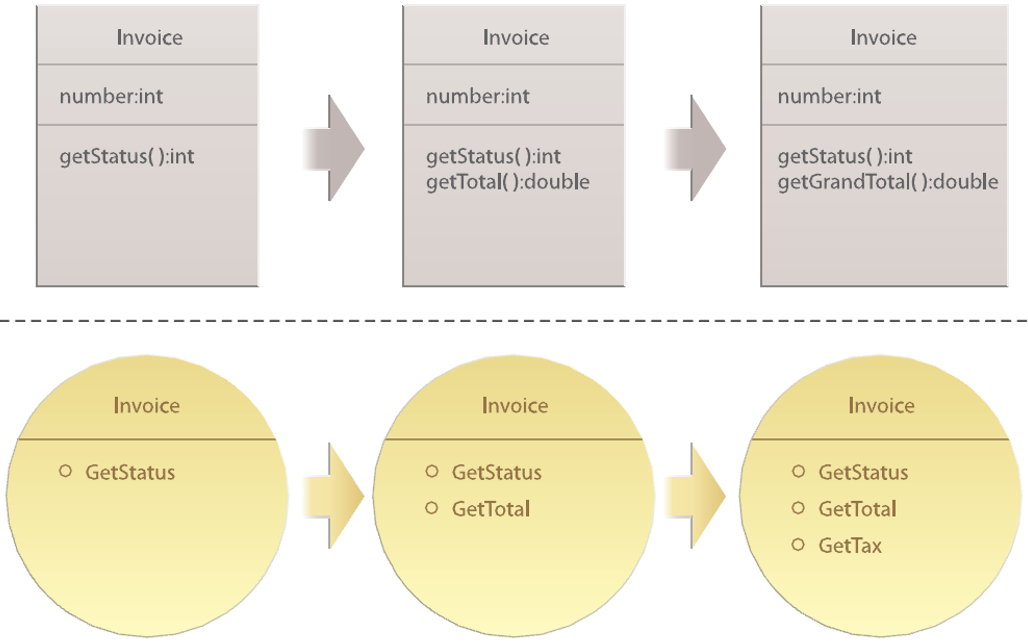
\includegraphics[width=0.97\linewidth]{images/开闭原则.png}
	\end{minipage}
	}
    \hfill
	\subfloat[别重复你自己]{
	\begin{minipage}[t]{0.4\linewidth}
	\centering
	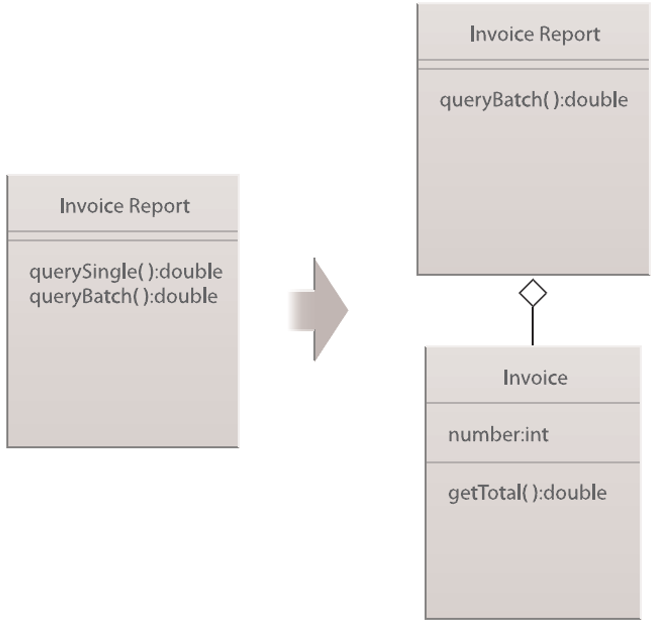
\includegraphics[width=0.97\linewidth]{images/别重复你自己.png}
	\end{minipage}
	}

    \subfloat[委托]{
	\begin{minipage}[t]{0.73\linewidth}
	\centering
	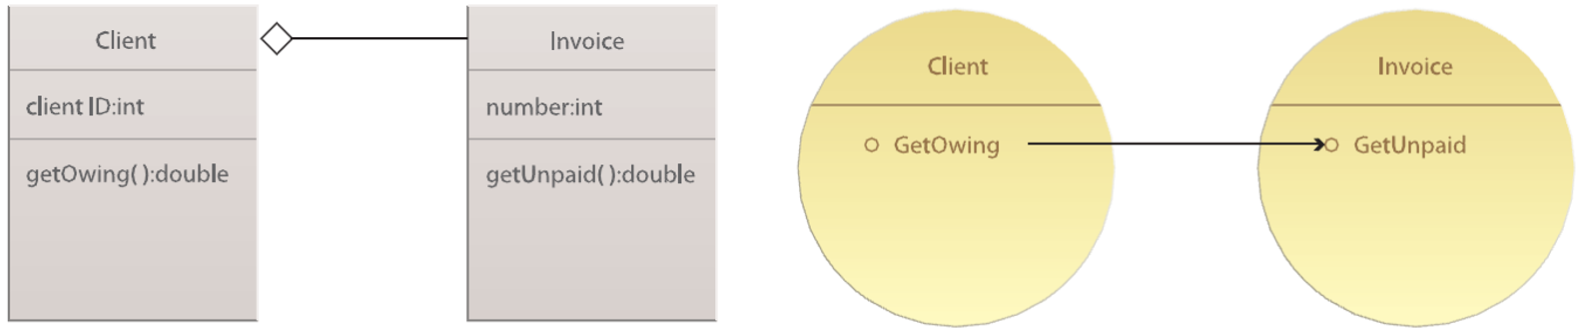
\includegraphics[width=0.97\linewidth]{images/委托.png}
	\end{minipage}
	}
	\centering
	\vspace{-1em}
\end{figure}

\begin{figure}[H]
	\setcounter{subfigure}{8}
	\centering
	\vspace{-0.5em}	
	\subfloat[关联]{
	\begin{minipage}[t]{0.75\linewidth}
	\centering
	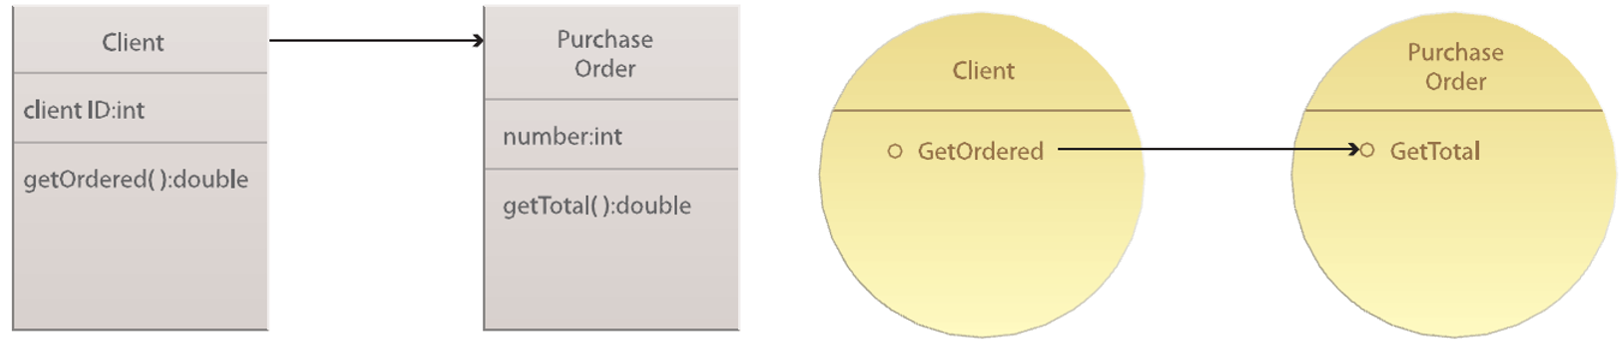
\includegraphics[width=0.97\linewidth]{images/关联.png}
	\end{minipage}
	}

    \subfloat[单一职责原则]{
	\begin{minipage}[t]{0.8\linewidth}
	\centering
	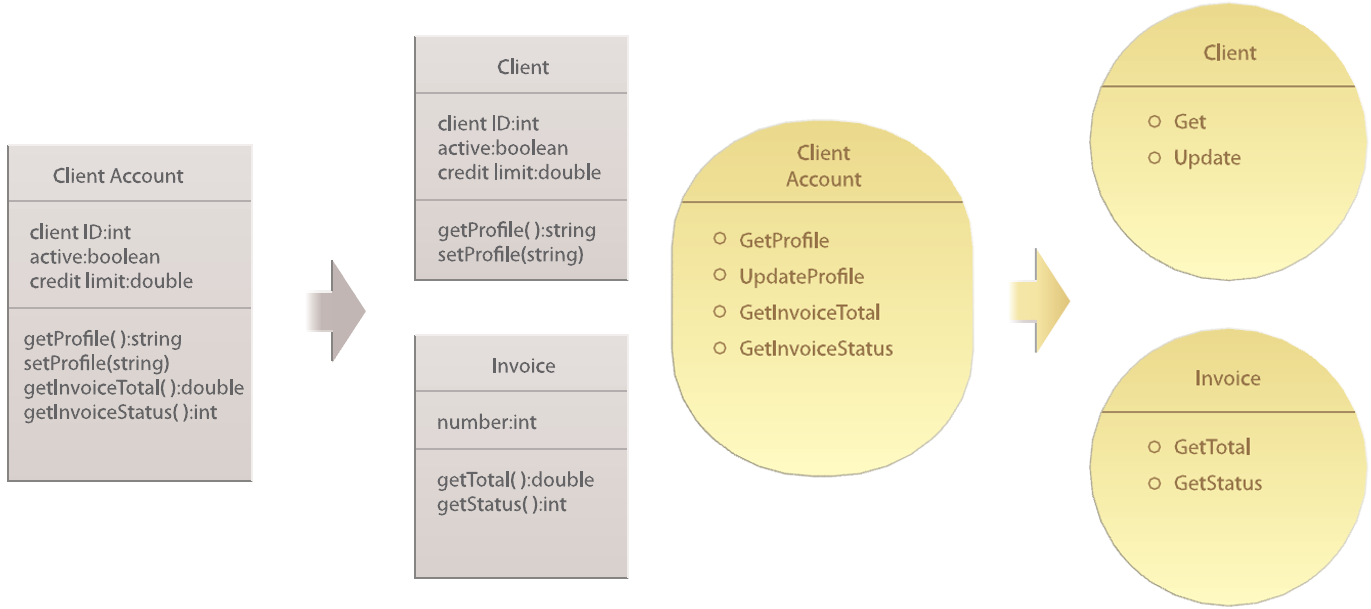
\includegraphics[width=0.97\linewidth]{images/单一职责原则.png}
	\end{minipage}
	}

    \subfloat[聚合]{
	\begin{minipage}[t]{0.47\linewidth}
	\centering
	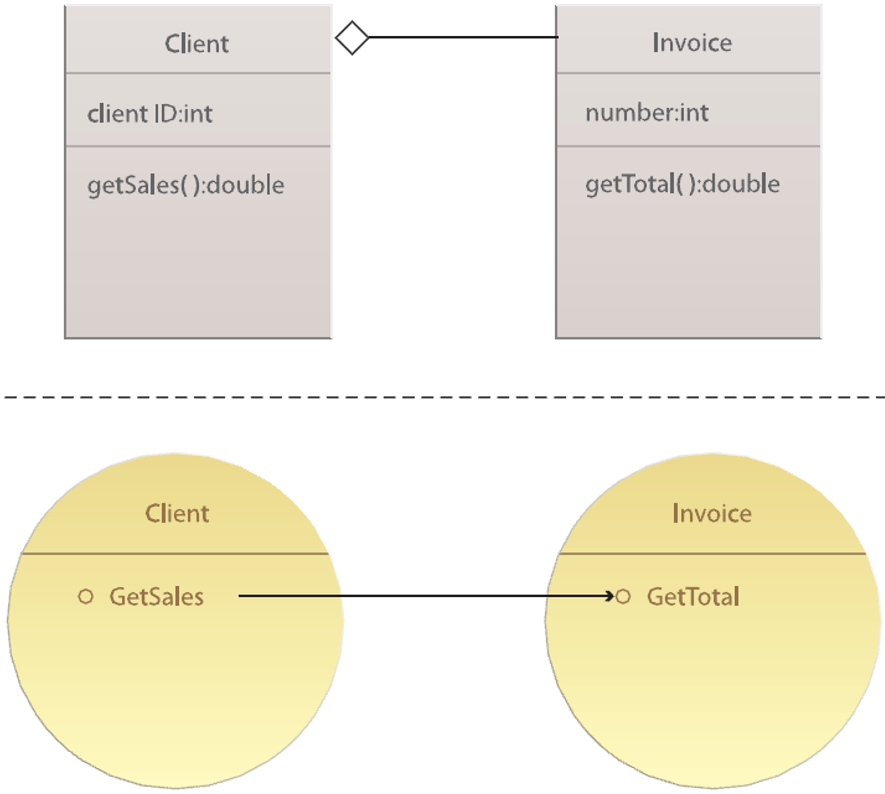
\includegraphics[width=0.97\linewidth]{images/聚合.png}
	\end{minipage}
	}
    \hfill
    \subfloat[组合]{
	\begin{minipage}[t]{0.4\linewidth}
	\centering
	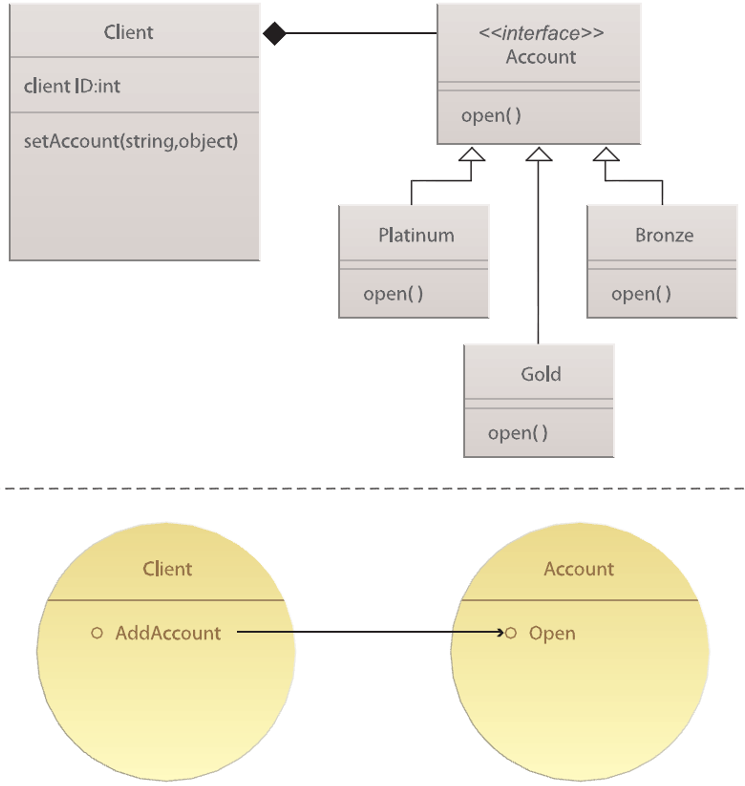
\includegraphics[width=0.97\linewidth]{images/组合.png}
	\end{minipage}
	}
	\centering
	\vspace{-1em}
\end{figure}
	\section{面向服务的架构}

\subsection{面向服务的架构概述}
面向服务的体系结构(SOA)是一种以业务为中心的IT体系结构方法,它支持将您的业务集成为链接的、可重复的业务任务或服务。SOA可帮助用户构建复合应用程序,复合应用程序是利用来自企业内外多个源的功能来支持水平业务流程的应用程序。

在软件工程中,SOA是一组原则和方法,用于以可互操作服务的形式设计和开发软件。这些服务是定义明确的业务功能,构建为软件组件(离散的代码片段和/或数据结构),可以重用于不同的目的。

\begin{itemize}
    \item SOA是从架构方面,整体支持面向服务泛型的基本概念性架构模型。
    \item SOA是一种业务-IT结合的方法。其中,应用依赖于现有的服务来实现业务过程。
    \item 服务是由服务提供商提供并由服务请求者使用的独立可重用软件组件。
    \item 实现SOA主要包括:
    \vspace{-0.8em}
    \begin{multicols}{2}
        \begin{itemize}
            \item 面向服务的企业
            \item 采用服务开发应用
            \item 采用服务对应用进行封装,以便今后的复用
            \item ……
    \end{itemize}
    \end{multicols}
    \vspace{-1em}
\end{itemize}

\begin{wraptable}{r}{6.5cm}
    \centering
    \vspace{-2.5em}
    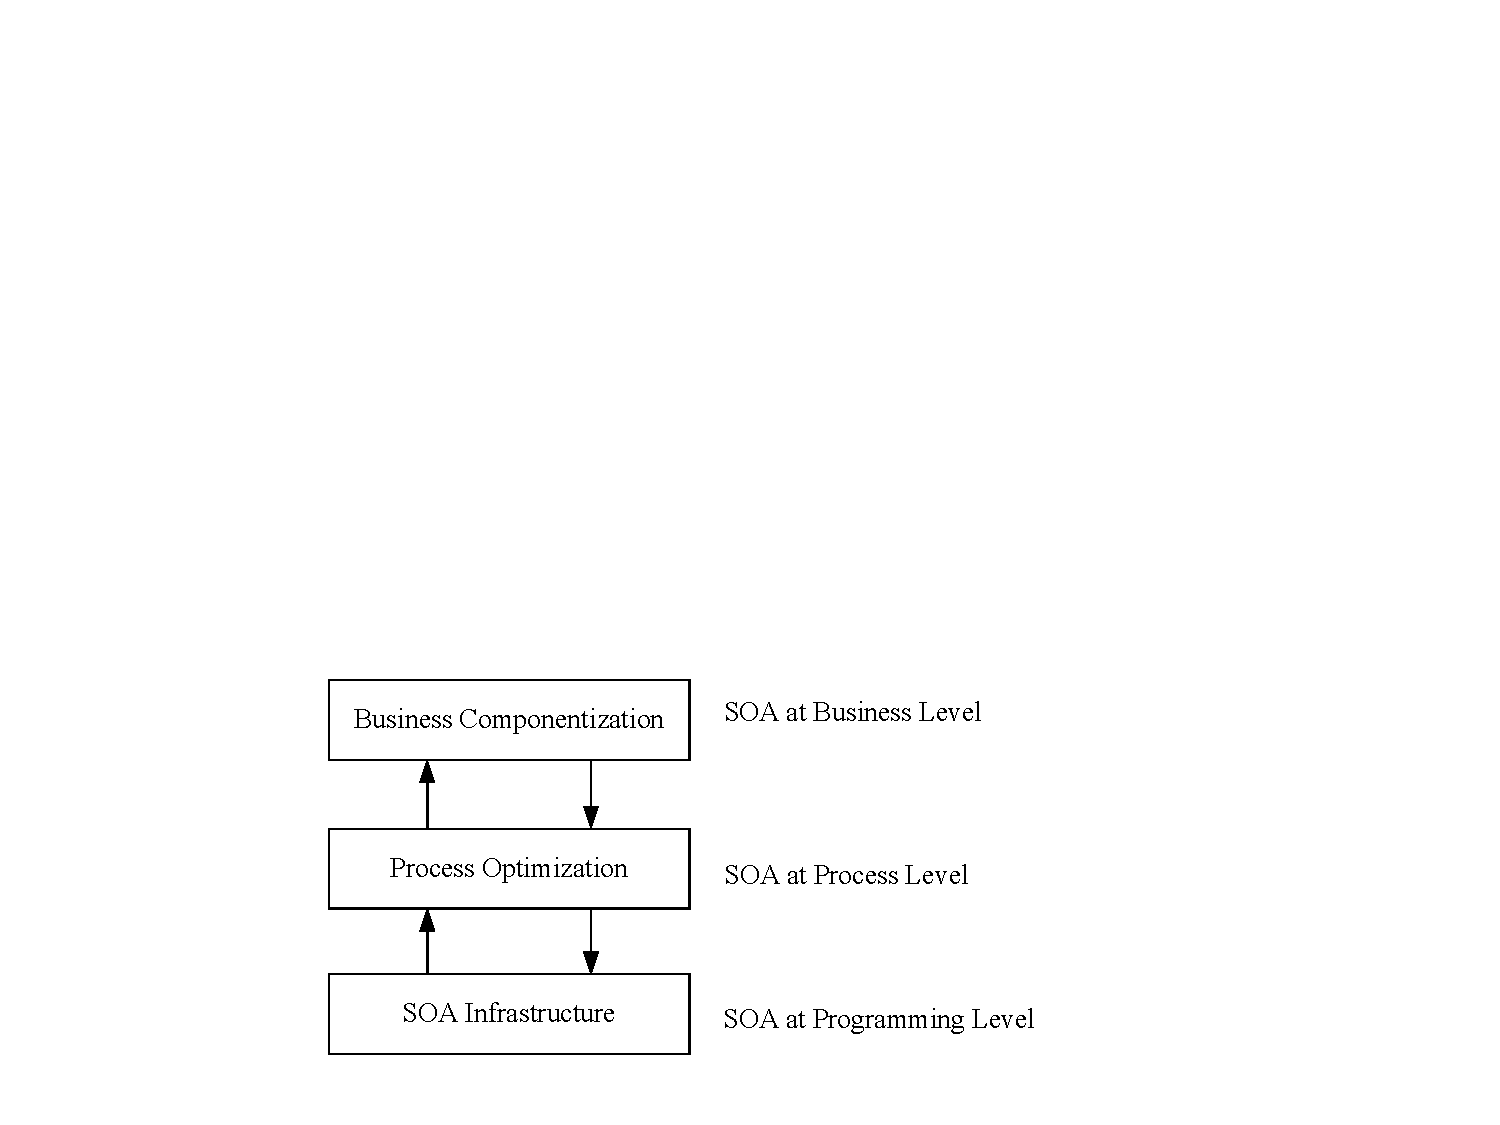
\includegraphics[width=5.5cm]{images/SOA结构.pdf}
    \vspace{-1.5em}
\end{wraptable}
$\ \checkmark\;$SOA解决方案构建在可从Internet或服务注册表访问的可重用服务之上

$\ \checkmark$以标准方式实现复杂软件系统的互操作性和集成

$\ \checkmark$连接IT和业务需求

SOA三角操作模型
\begin{figure}[H]
    \vspace{-0.5em}
	\centering
	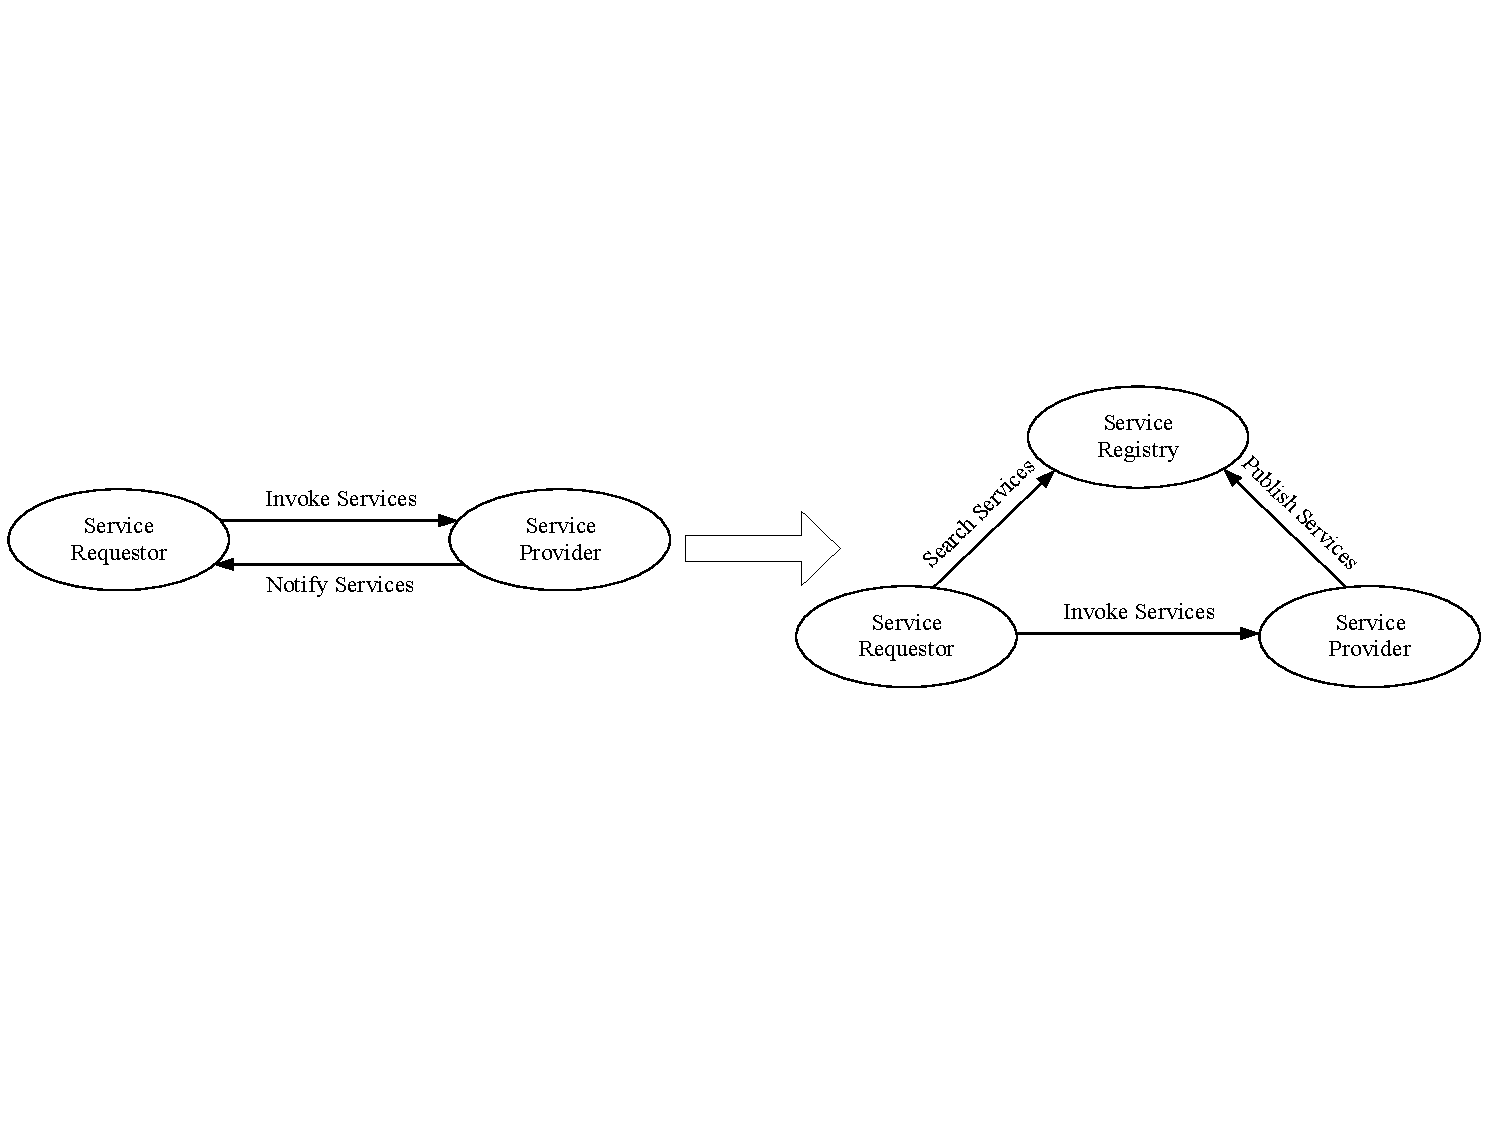
\includegraphics[width=0.85\textwidth]{images/SOA三角操作模型.pdf}
    \vspace{-1em}
\end{figure}

\subsection{SOA的特点}
SOA的优点:
\begin{itemize}
    \item 从IT角度出发
    \begin{itemize}
        \item 松耦合,消除假依赖(复用):语言、平台和厂商中立;消除时间依赖;消除访问地址依赖;消除访问协议依赖
        \item 服务间接寻址(灵活)
    \end{itemize}
    \item 从业务角度出发
    \vspace{-0.8em}
    \begin{multicols}{2}
        \begin{itemize}
            \item 保护企业投资,提升现有IT资源的作用,促进IT资源的复用
            \item 提高企业灵敏度
            \item 支持企业外包管理模式
        \end{itemize}
    \end{multicols}
    \vspace{-1em}
\end{itemize}

从双角度出发,SOA在不同粒度上提供了本质性的指导:业务层、过程层、中间件层和编程层
\begin{itemize}
    \item 在每个层次中间,SOA 按照自顶向下的方式,将一个较大的单元分解为较小、以服务为中心的单元
    \item 按照自底向上的方式,将可供使用的较小单元组织成为较大的单元,用以提供全新的服务
\end{itemize}

\begin{figure}[H]
    \vspace{-0.5em}
	\centering
	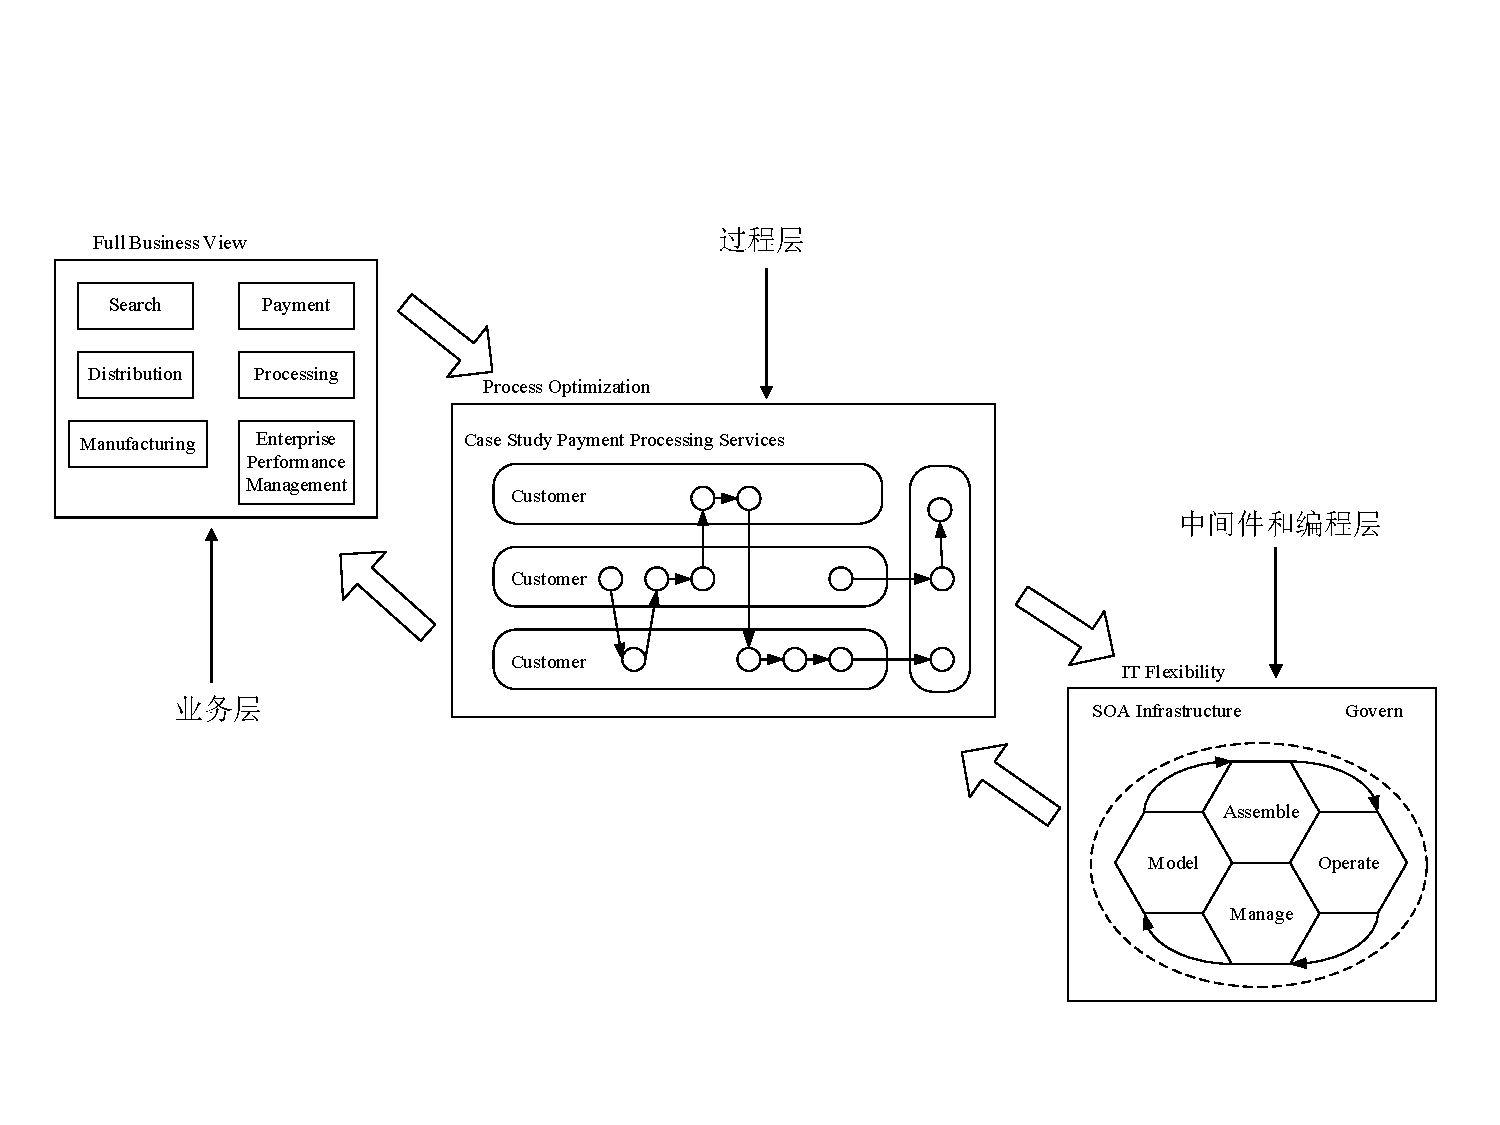
\includegraphics[width=\textwidth]{images/SOA双角度.pdf}
    \vspace{-1em}
\end{figure}

\begin{itemize}
    \item 在编程层,SOA可用于指导低级IT技术
    \begin{itemize}
        \item 简单对象访问协议(Simple Object Access Protocol, SOAP)
        \item 用于数据传输的二进制SOAP消息传递
        \item 服务组件体系结构(Service Component Architecture, SCA,一种编程模型)
    \end{itemize}
    \item 在中间件层,SOA可用于指导通用产品和开源软件的设计和开发
    \begin{itemize}
        \item 从不同的模型中进行选择:例如ESB (Enterprise Service Bus,单个企业服务总线)或多个 ESB、面向消息或基于事件的基础架构
    \end{itemize}
    \item 在过程层,SOA可用于指导业务流程集成和管理,以及事件驱动架构的设计
    \item 在业务层,SOA可用于组件化企业并支持高级转型咨询
    \begin{itemize}
        \item 帮助高管决定是使用SOA服务包实现业务流程,还是使用SOA概念将业务流程划分为子流程
    \end{itemize}
\end{itemize}

\vspace{-0.5em}
\begin{shaded}
\subsubsection*{企业服务总线(ESB)}
\begin{itemize}
    \item ESB是一个概念性的软件基础结构,它促进服务组件及其交互的动态集成、消息路由、中介和控制。
    \item 与通用对象请求代理体系结构(CORBA)对象总线相比,它集成了面向对象的软件组件和Java 2平台企业版(J2EE)应用程序服务器;ESB 在概念上集成了服务和服务组件。
    \item ESB提供了一个基础结构,从集成和消息传递的角度支持服务组件的互操作性和可重用性。
\end{itemize}

ESB的基本形式:
\vspace{-0.8em}
\begin{multicols}{4}
    \begin{itemize}
        \item 集成
        \item 消息路由
        \item 转换
        \item 管理
    \end{itemize}
\end{multicols}
\vspace{-1em}

高级ESB通常提供许多额外的增值功能:
\vspace{-0.8em}
\begin{multicols}{2}
    \begin{itemize}
        \item 用于服务发现和配置的工具
        \item 根据性能和错误事件动态调整服务级别协议
        \item 高级Web服务发现
        \item 适用于现有或新兴技术的特定适配器
    \end{itemize}
\end{multicols}
\vspace{-1em}

\begin{figure}[H]
    \vspace{-0.5em}
	\centering
	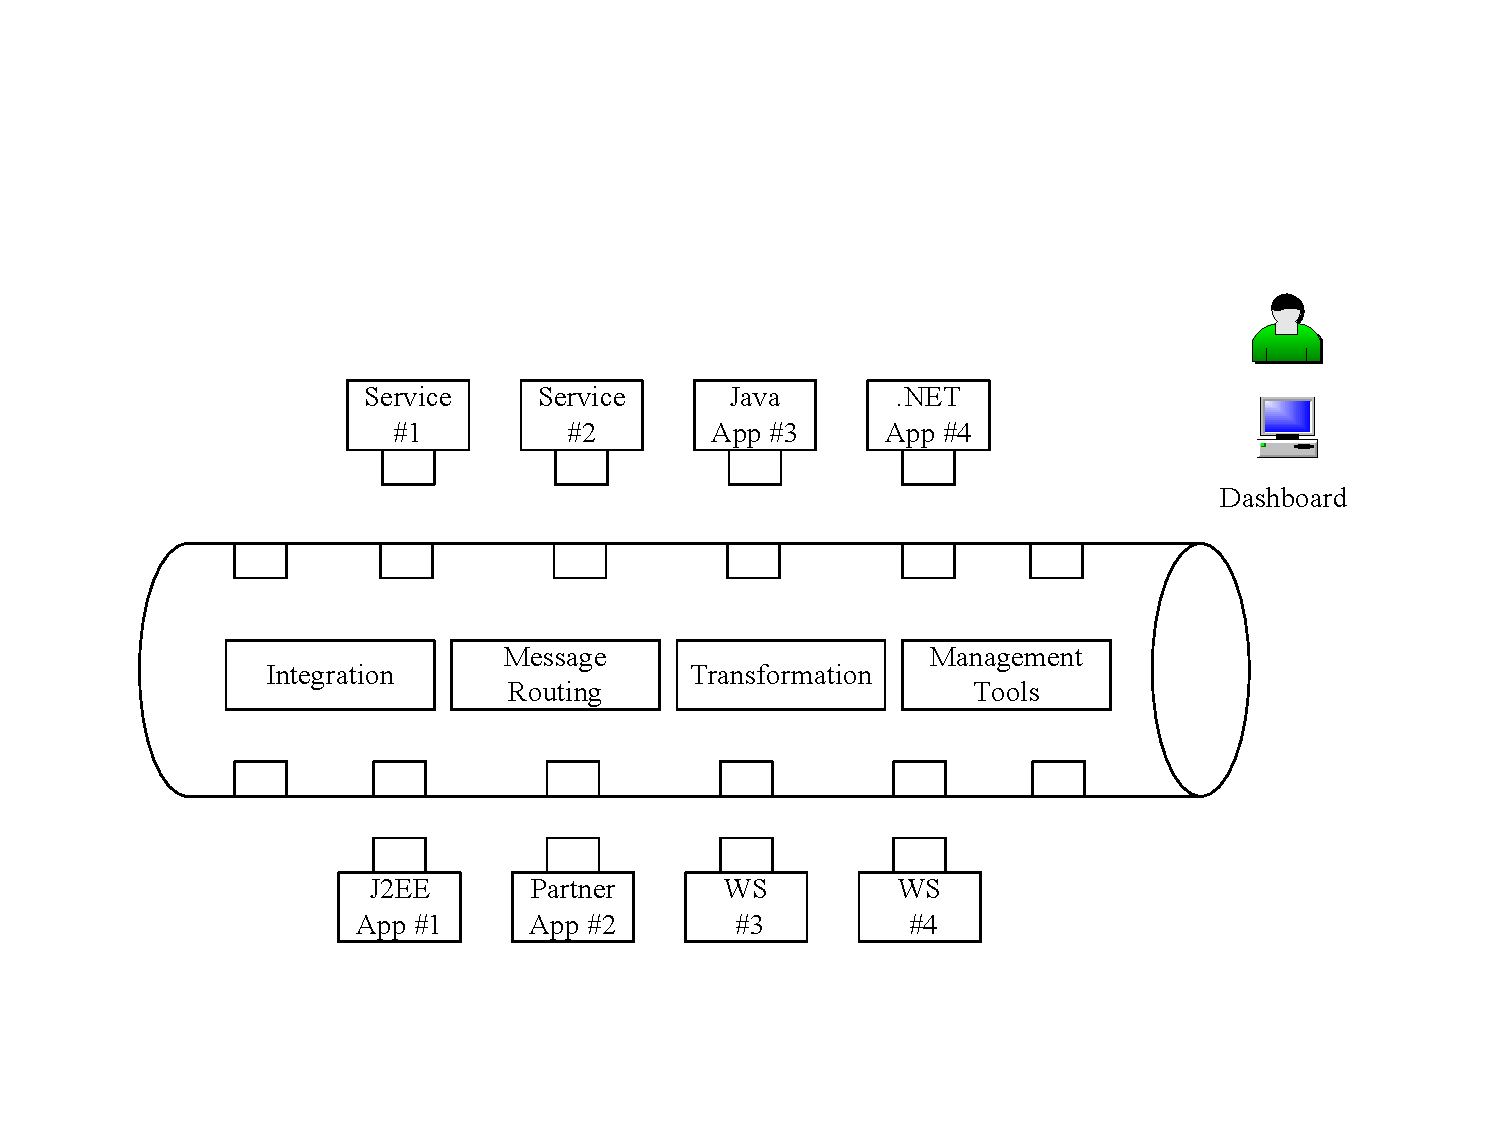
\includegraphics[width=0.65\textwidth]{images/ESB.pdf}
    \vspace{-1em}
\end{figure}

\end{shaded}
\vspace{-1em}

\subsection{SOA参考架构}
\begin{figure}[H]
    \vspace{-0.5em}
	\centering
	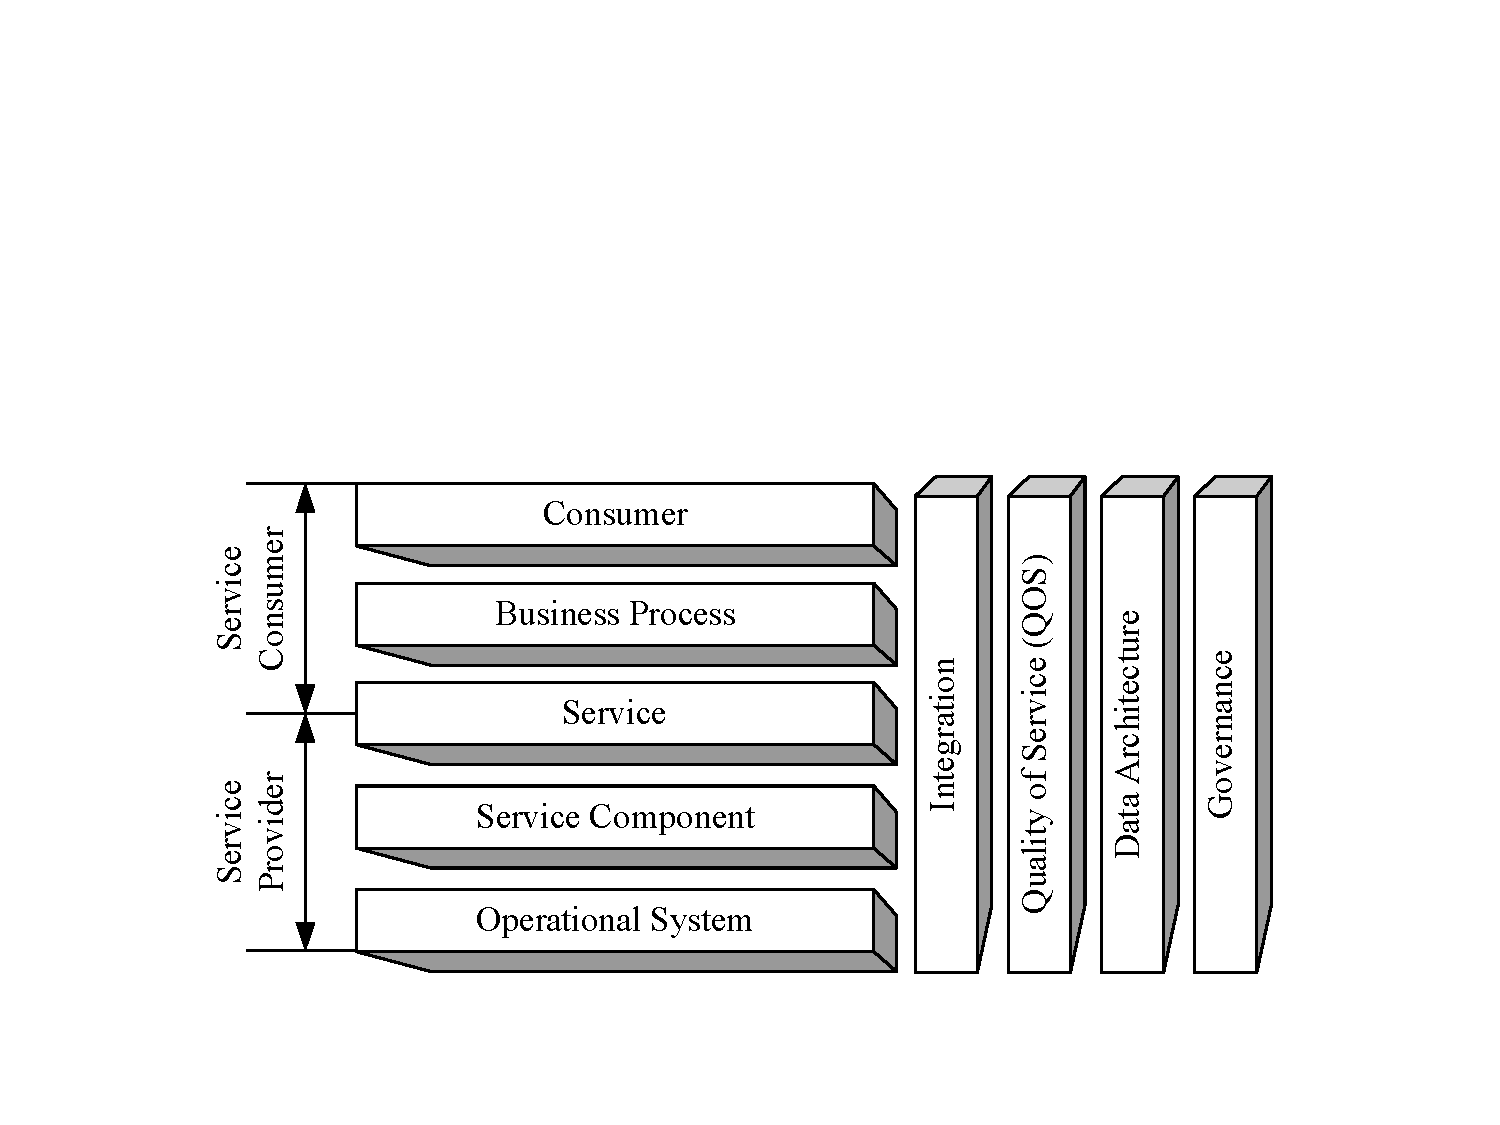
\includegraphics[width=0.7\textwidth]{images/SOA参考架构.pdf}
    \vspace{-1em}
\end{figure}

水平层:对功能性需求加以满足,五个水平层分为服务提供者和服务消费者两组:
\begin{itemize}
    \item 服务提供者(后台)
\end{itemize}
\begin{spacing}{1.2}
    \begin{table}[H]
    \centering
    \vspace{-0.5em}
    \begin{tabular}{|c|l|}
        \hline
        \textbf{操作型系统层} & \begin{tabular}[c]{@{}l@{}}包括ISV(独立软件开发商)提供的打包应用、客户应用、遗留系统等。\\ 该层的应用(不一定面向服务)往往只为一个目的、服务于一类特定用户。\end{tabular}                                                                                                                                         \\ \hline
        \textbf{服务组件层}  & \begin{tabular}[c]{@{}l@{}}包括用于提供用以实现服务层中所定义服务的代码容器,其中一个服务组件依赖于\\ 操作系统型层次中的一些打包组件、服务层中的一些服务、业务过程层中的一些业\\ 务过程。\\ 该层可能实现多个方法,但其中只有一部分会被服务层封装为服务。\\ 从调用角度出发,服务组件层负责完成输入转换和输出配置的自动化逻辑。\end{tabular}                                                       \\ \hline
        \textbf{服务层}    & \begin{tabular}[c]{@{}l@{}}将SOA三角操作模型扩展为综合的逻辑层次,以支持服务注册、服务分解、服务\\ 发现、服务绑定、接口聚合和生命周期管理。服务层负责定位合适的服务提供者,\\ 并绑定到具体目标服务接口;同时负责以服务组合的形式封装服务对外提供。\\ \textbf{服务簇}是服务层中的核心概念,是一类从概念上服务于同一业务功能的服务集合。\\ 服务簇中的服务可以由不同的功能提供者所发布,并在具体的特性上有所差异(但\\ 都能满足业务功能需求)。\end{tabular} \\ \hline
    \end{tabular}
\end{table}
    \vspace{-2.5em}
\end{spacing}

\begin{itemize}
    \item 服务消费者(前台)
\end{itemize}

\begin{spacing}{1.15}
    \begin{table}[H]
    \centering
    \begin{tabular}{|c|l|}
    \hline
    \textbf{服务层}   & 服务层作为前后台连通的接口,功能同上。   \\ \hline
    \textbf{业务过程层} & \begin{tabular}[c]{@{}l@{}}以组合和分解的方式来处理业务逻辑。\\ 从组合角度出发,业务过程层使用服务层来快速组合服务,并协调业务过程来满足消\\ 费者需求;从分解的角度出发,业务过程层将业务需求分解为能够由概念上的服务簇\\ 所表达的任务。\\ 业务服务层着眼于从协作和管理一些列过程的角度出发,采用也无流程来构建SOA\\解决方案。\\ 存在两种组合方式:编排和编导(二者功能上等价,主流模式为编排)。\end{tabular} \\ \hline
    \textbf{消费者层}  & \begin{tabular}[c]{@{}l@{}}消费者层负责表达对业务过程层、服务层及其他层次的调用。\\ 通过为业务服务快速构建用户接口来满足消费者的需求。\\ 消费者层负责构建SOA解决方案与用户之间进行交互的前端接口。\\ 消费者层可能需要同时支持不同种类的用户和渠道。\\ 为了提升展现性能,往往需要支持缓存机制。\end{tabular}                                                         \\ \hline
    \end{tabular}
\end{table}
    \vspace{-1em}
\end{spacing}

\begin{figure}[H]
	\setcounter{subfigure}{0}
	\centering
	\vspace{-0.5em}	
	\subfloat[编排]{
	\begin{minipage}[t]{0.46\linewidth}
	\centering
	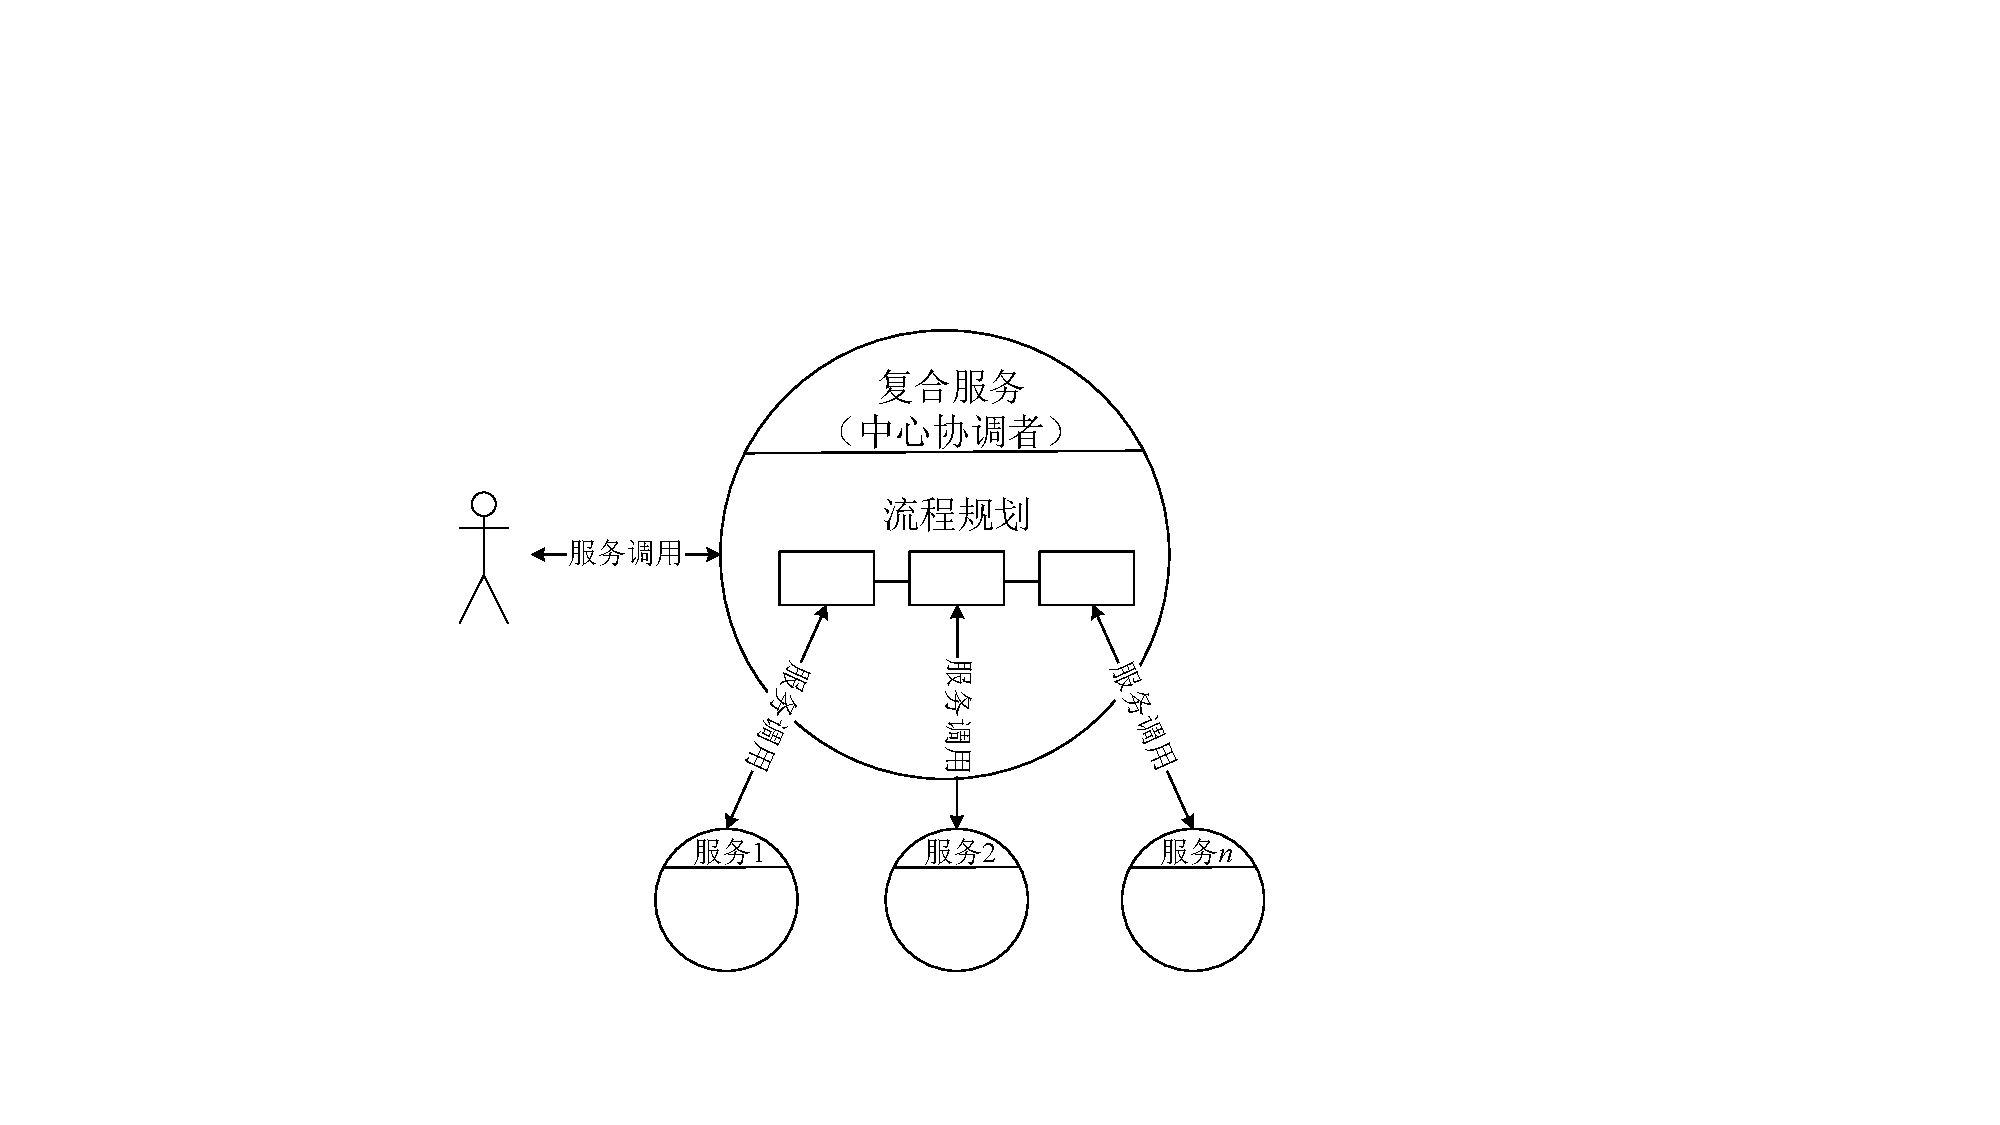
\includegraphics[width=0.97\linewidth]{images/编排.pdf}
	\end{minipage}
	}
    \hfill
	\subfloat[编导]{
	\begin{minipage}[t]{0.47\linewidth}
	\centering
	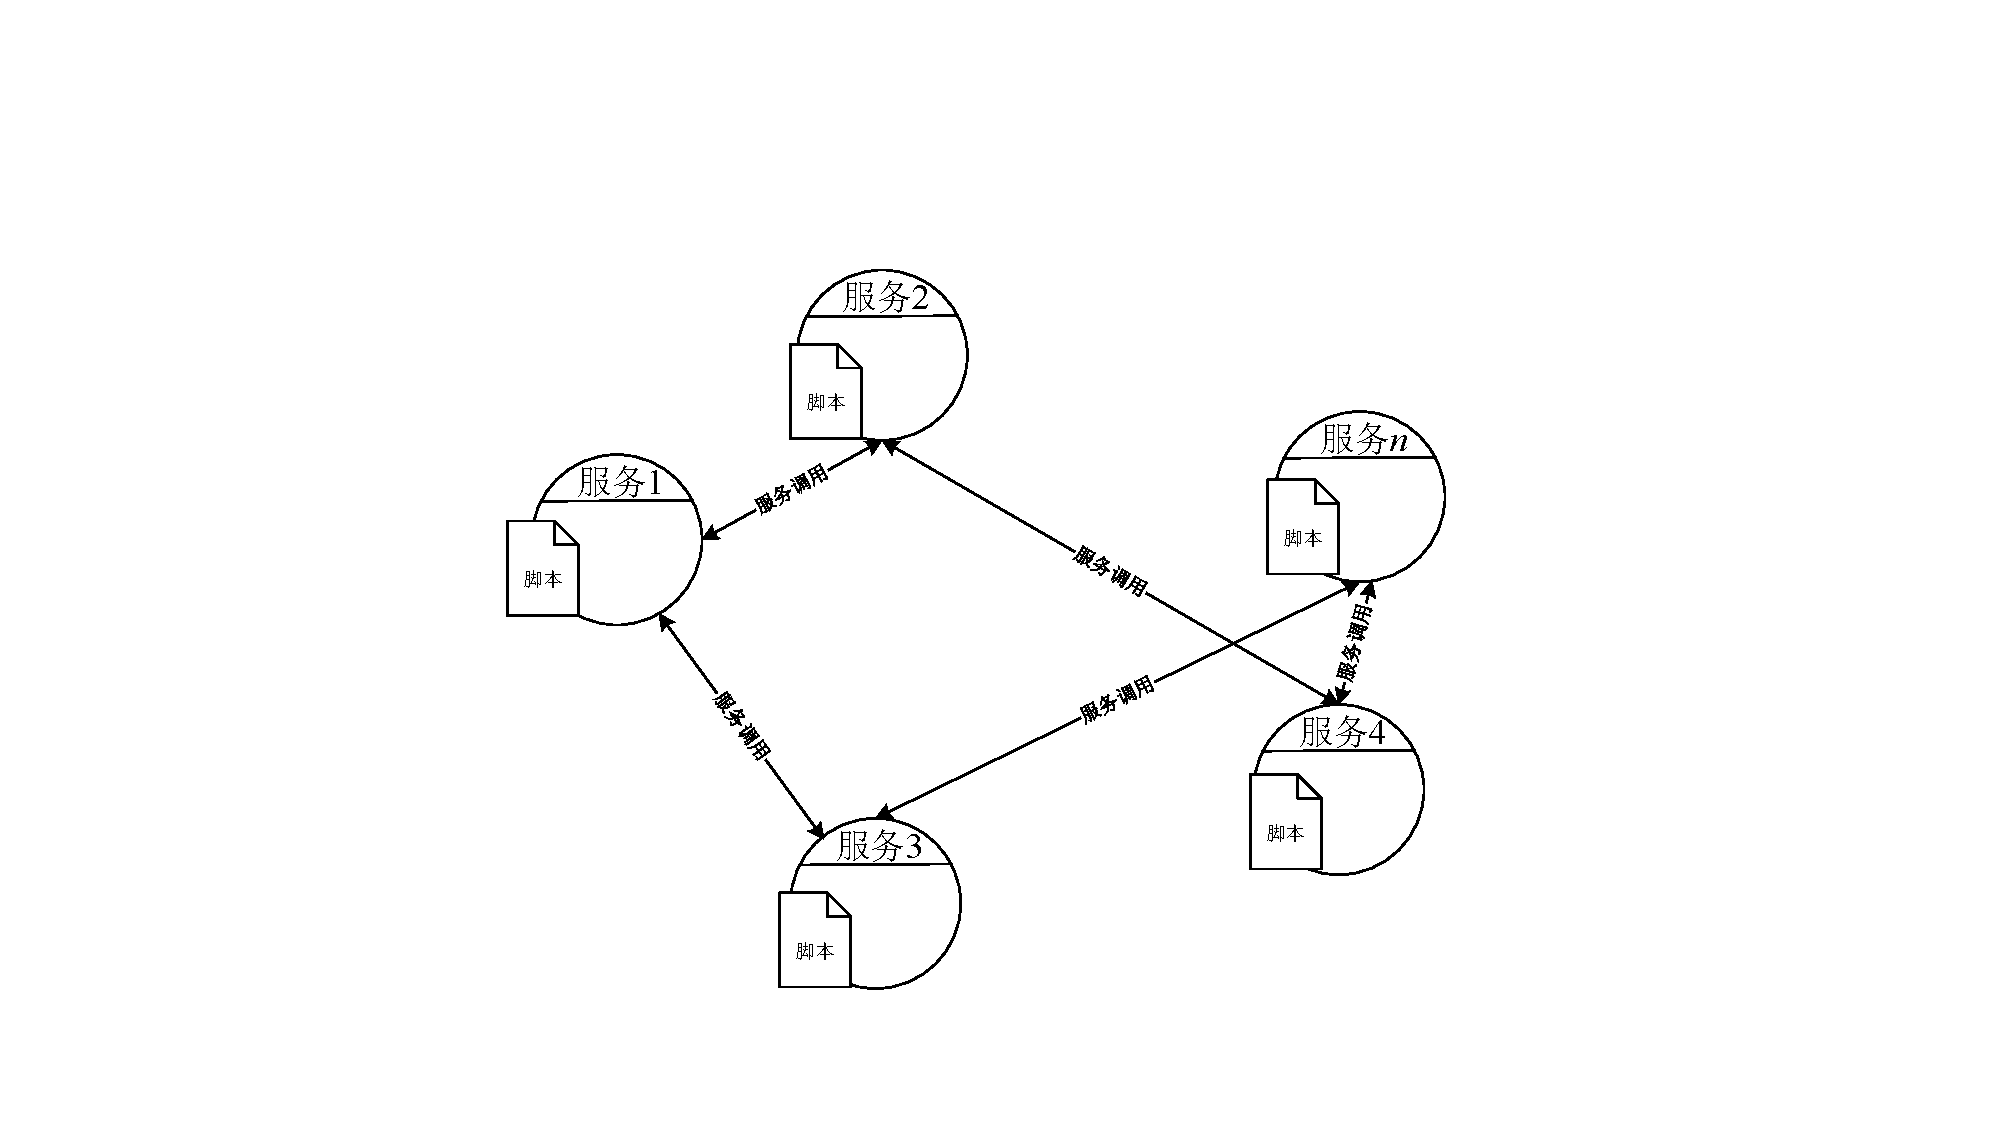
\includegraphics[width=0.97\linewidth]{images/编导.pdf}
	\end{minipage}
	}
	\centering
	\vspace{-1em}
\end{figure}

垂直层:对当前系统进行支撑以及实现服务质量、非功能性需求
\begin{spacing}{1.15}
        \begin{table}[H]
        \centering
        \resizebox{\textwidth}{!}{
        \begin{tabular}{|c|l|}
        \hline
        \textbf{集成层}                                                   & \begin{tabular}[c]{@{}l@{}}SOA解决方案中的关键支持部件,用以在服务请求者和服务提供者之间,完成服务请求的 \\ 中介、路由和转换。\end{tabular}                                                 \\ \hline
        \textbf{\begin{tabular}[c]{@{}c@{}}服务质量层\\ (QoS)\end{tabular}} & \begin{tabular}[c]{@{}l@{}}从各个方面(可用性、可靠性、安全性等非功能性需求)提供解决方案层级的QoS管理。\\ 服务质量层不关注于服务层级的QoS控制,而是着眼于为解决方案层级的 QoS 控制提供 \\ 支持、跟踪、监视和管理。\end{tabular} \\ \hline
        \textbf{数据架构层}                                                 & \begin{tabular}[c]{@{}l@{}}为了方便值链集成(集成来源于不同开发方的服务),数据架构层为领域相关的数据架构提 \\ 供统一的表达和支持机制。\end{tabular}                                             \\ \hline
        \textbf{治理层}                                                   & \begin{tabular}[c]{@{}l@{}}提供用以确保 SOA 解决方案的设计原则;通常使用最佳实践的方式,来提供如何在各个层 \\ 次中构建 SOA 解决方案的原则、如何监管运营中的系统,并在运行时处理异常的原则。\end{tabular}               \\ \hline
        \end{tabular}}
    \end{table}
    \vspace{-2em}
\end{spacing}

\begin{itemize}
    \item SOA-RA 展示了如何将 SOA 解决方案构建为一组逻辑层的抽象。
    \item SOA-RA 是一种松耦合的架构,因为每个层不严格隐藏在上面的层之中。
    \item SOA-RA 是一个企业级架构模板,通过定义参考架构指导在企业级别上创建 SOA 解决方案。
    应用 SOA-RA 模型来定义 SOA 导向的系统架构的一种实践称为服务导向建模和架构(SOMA)。
    \item 在SOA-RA层中配置组件定义了三个步骤:
    \vspace{-0.8em}
    \begin{multicols}{3}
    \begin{itemize}
        \item 服务识别步骤
        \item 服务规范步骤
        \item 服务实现步骤
    \end{itemize}
    \end{multicols}
    \vspace{-1em}
\end{itemize}

\subsection{SOA解决方案生命周期}
服务的生命周期是指从服务开始构思到该服务不再使用时结束的时间段。
\begin{figure}[H]
    \vspace{-0.5em}
	\centering
	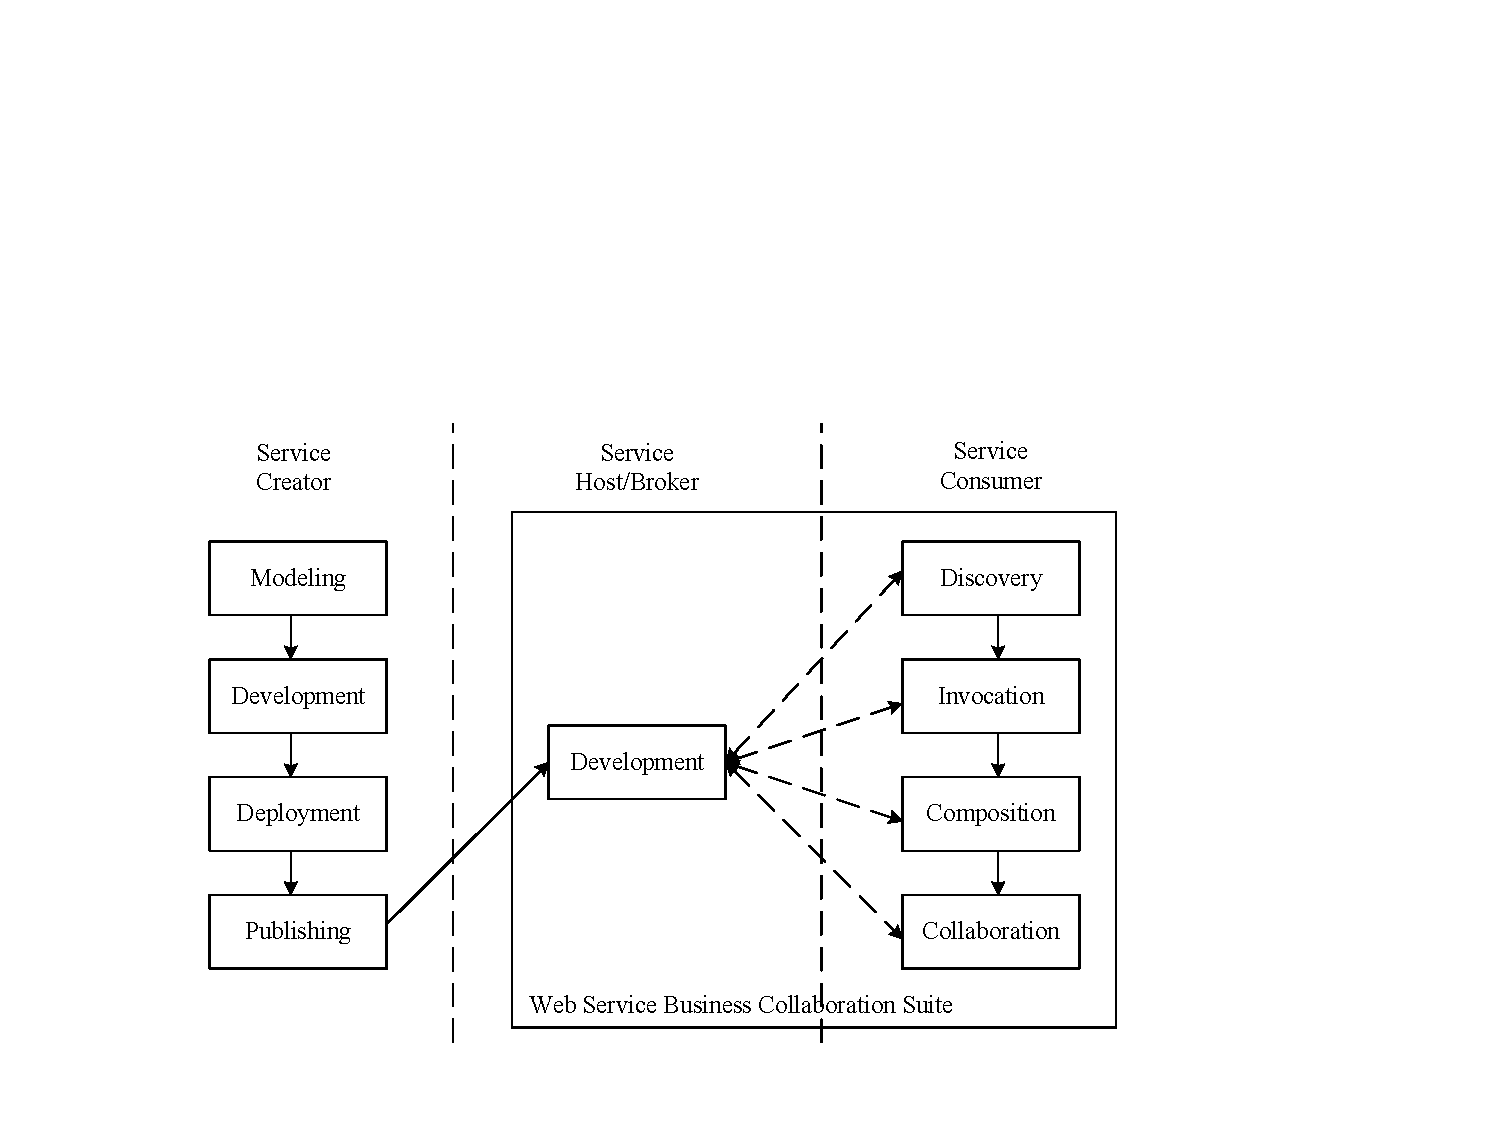
\includegraphics[width=0.65\textwidth]{images/SOA Solution Lifecycle.pdf}
    \vspace{-1em}
\end{figure}

\vspace{-0.5em}
\begin{spacing}{1.2}
\centering
    \begin{longtable}{|m{2.5cm}<{\centering}|m{12cm}|}
    \hline
    服务模型(Services modeling) & 
    \vspace{-1.3em}
    \begin{itemize}[leftmargin=1.5em,itemsep=-2pt]
        \item 使用概念建模技术设计服务
        \item 基于WSDL的自顶向下分解方法是一种服务建模方法
        \item 该方法与传统的接口优先设计方法没有区别
        \item OMG\footnote{OMG(Object Management Group),它是一个国际性的计算机工业标准组织,负责制定和维护各种计算机标准,包括UML和MDA等。该组织致力于推广面向对象技术和相关标准,并促进不同系统之间的互操作性。}的基于UML的模型驱动架构(MDA)可以用于使用Web服务和SOA建模业务解决方案的复杂性
    \vspace{-1.5em}
    \end{itemize} \\ \hline
    开发(Development) & 
    \vspace{-1.3em}
    \begin{itemize}[leftmargin=1.5em,itemsep=-2pt]
        \item 服务的详细实现可以使用任何编程语言来实现(例如Java、C\#和C++)
        \item 服务的开发阶段涉及典型软件生命周期的几个阶段,包括设计、开发和测试
        \item 软件开发方法论可以用于指导开发过程
    \vspace{-1.5em}
    \end{itemize} \\ \hline
    Deployment & \multicolumn{1}{c|}{部署}  \\ \hline
    Publishing & \multicolumn{1}{c|}{发布}  \\ \hline
    Discovery & \multicolumn{1}{c|}{发现服务}  \\ \hline
    调用(Invocation) & 
    \vspace{-1.3em}
    \begin{itemize}[leftmargin=1.5em,itemsep=-2pt]
        \item 通常情况下,服务请求者和服务提供者会就服务级别协议(SLA)进行协商
        \item 在达成共识之后,服务请求者调用所需的Web服务,并在服务提供者现场远程执行服务
        \item SOAP是承载请求和响应的典型协议,需要进行信息的编组和解组
    \vspace{-1.5em}
    \end{itemize} \\ \hline
    组合(Composition) & 
    \vspace{-1.3em}
    \begin{itemize}[leftmargin=1.5em,itemsep=-2pt]
        \item 自适应地将一组可用的Web服务组合成业务流程。
        \item BPEL4WS\footnote{Business Process Execution Language for Web Services,即Web服务业务流程执行语言。它是一种基于XML的编程语言,用于描述在Web服务环境中运行的业务流程,可以协调多个Web服务的协作,实现复杂的业务逻辑。}和Web服务编排接口(WSCI)用于描述这种组合。
    \vspace{-1.5em}
    \end{itemize} \\ \hline
    协作(Collaboration) & 在一个全面的业务流程中,通常会有多个服务由不同的服务提供者提供和调用。
    为了协调它们,它们之间的信息交换和协作是必要的。 \\ \hline
    通过分析控制进行监控和管理(Monitoring and Management with analytical control) & 
    \vspace{-1.3em}
    \begin{itemize}[leftmargin=1.5em,itemsep=-2pt]
        \item 在网络环境中,应监控和控制Web服务的执行
        \item 包括访问控制、性能监控、服务级别协议(SLA)执行和异常处理
        \item 我们应该在涉及多个方的分布式环境中监控和跟踪交换信息的状态
        \item 这个过程可能跨越多个组织,因此需要联合访问控制策略
        \item 进行数据分析和信息分析以改进
    \vspace{-1.5em}
    \end{itemize} \\ \hline
\end{longtable}
\end{spacing}


	\section{面向服务中的信息交换和数据类型}

\subsection{电子信息交换}
电子信息交换是指在执行领域(业务)相关功能时,各式各样、采用电子方式编码的信息,在软件单元之间的移动的过程。

\begin{figure}[H]
    \vspace{-0.5em}
	\centering
	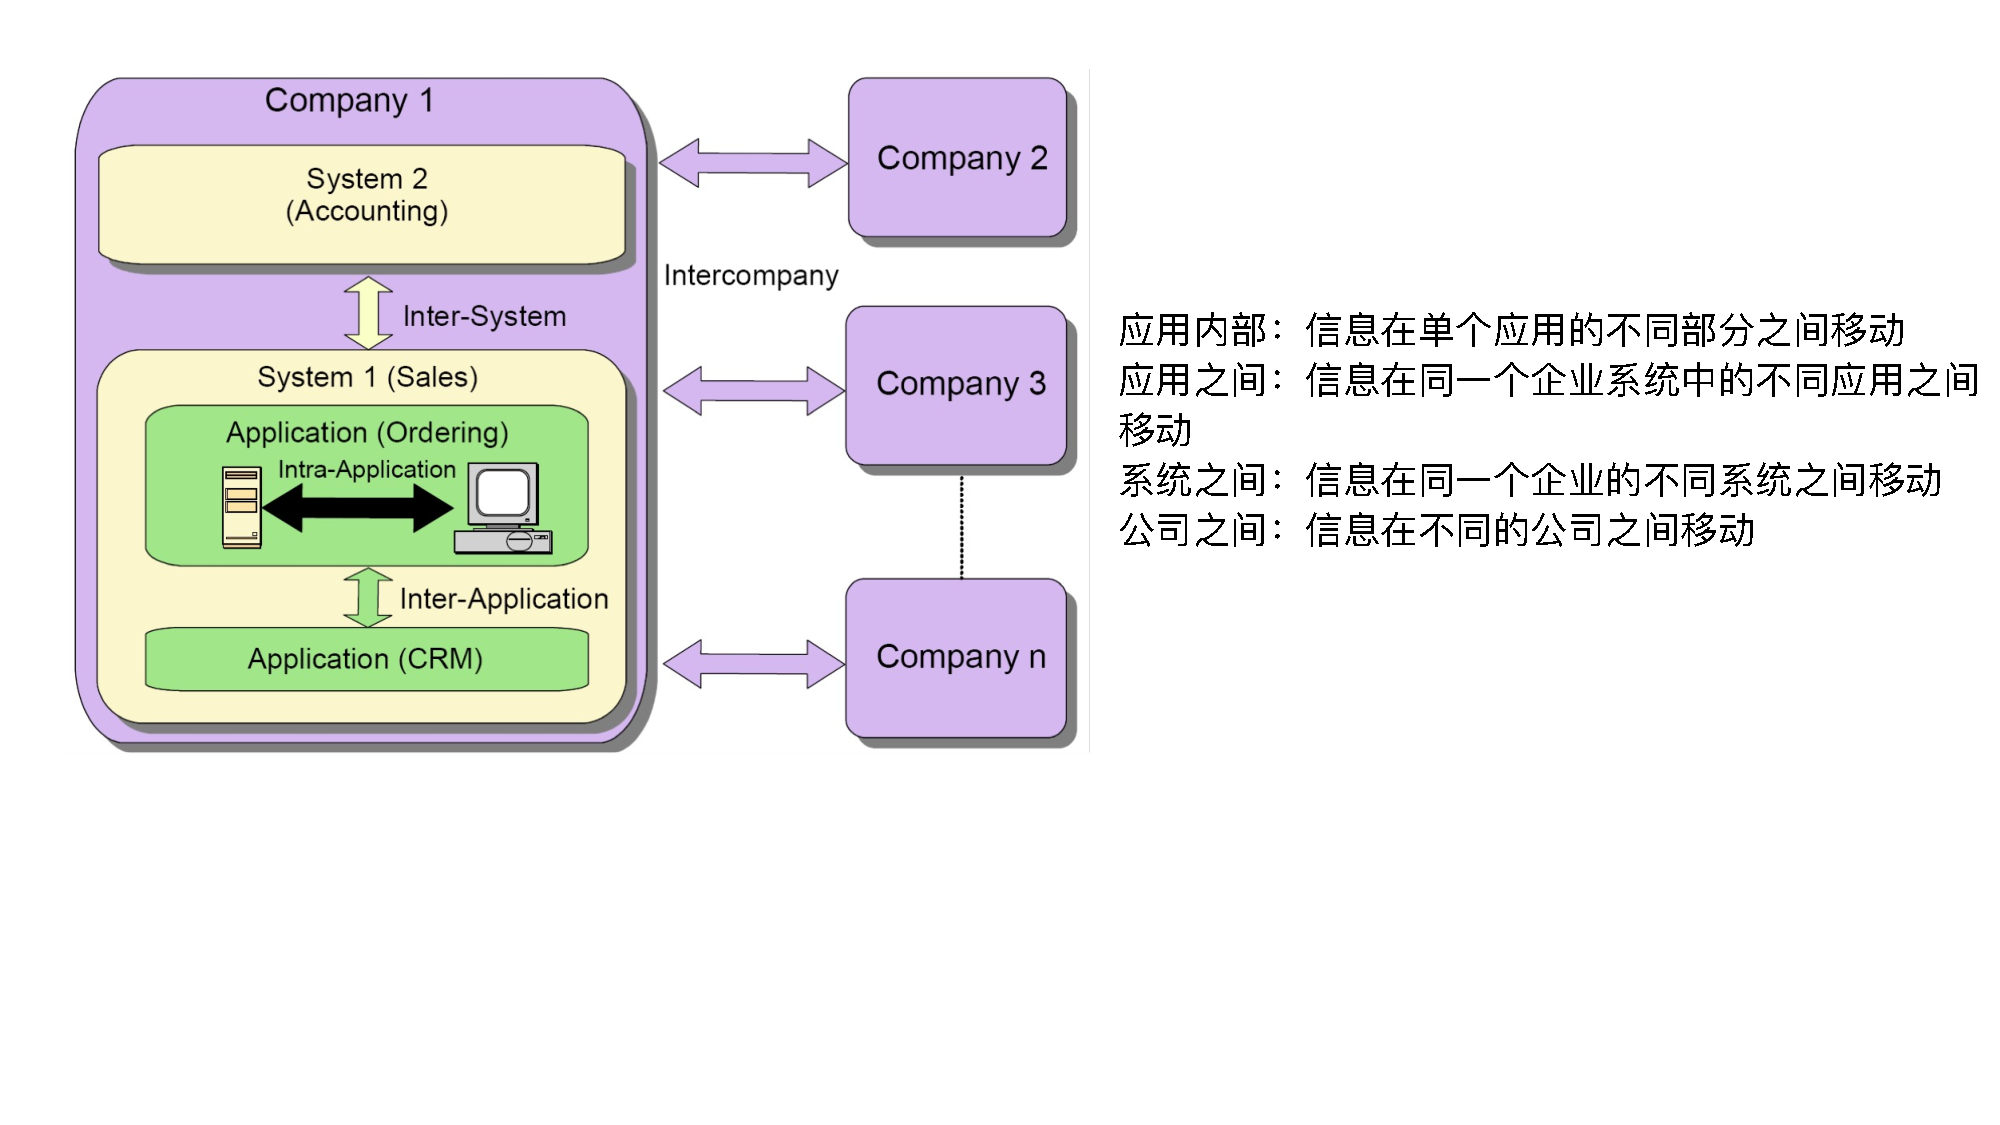
\includegraphics[width=0.95\textwidth]{images/Electronic Information Exchange.pdf}
    \vspace{-1em}
\end{figure}

服务计算中的数据类型
\vspace{-0.8em}
\begin{multicols}{2}
    \begin{itemize}
        \item 使用 XML 消息发布/发现/调用服务
        \item XML 消息交换中的另一个问题是数据类型
        \item 一种方法是用XML 架构脚本验证 XML 消息
        \item 一组XML模式脚本可以在特定的行业中被接受并通过互联网发布,这可以被视为“数据类型标准”
    \end{itemize}
\end{multicols}
\vspace{-1em}

\subsection{XML}
\begin{wraptable}{r}{6.5cm}
    \centering
    \vspace{-1.5em}
    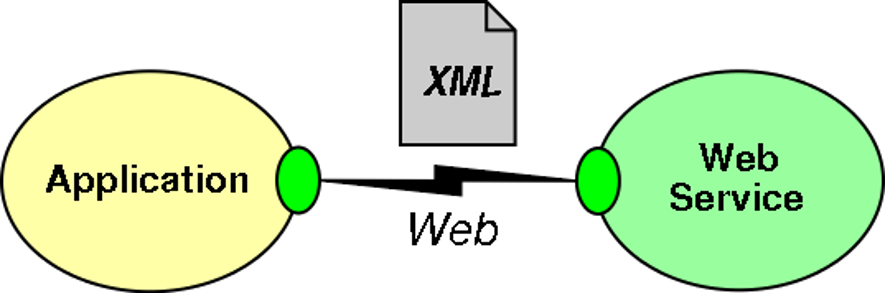
\includegraphics[width=6cm]{images/XML.png}
    \vspace{-1.5em}
\end{wraptable}
XML 是满足一组良好定义规则的格式化文本,主要由标签和文本构成,可以被储存和展现为诸如通过 HTTP 传输的消息、编程语言中的字符串、数据库中的 CLOB(character large object)等文本数据形式。为了方便起见,XML 文档也被用来指应用之间的字节流、数据库中的字段、XML 信息集中的对象集合。

\subsubsection{XML的结构}
XML文档为树状结构
\begin{figure}[H]
    \vspace{-0.5em}
	\centering
	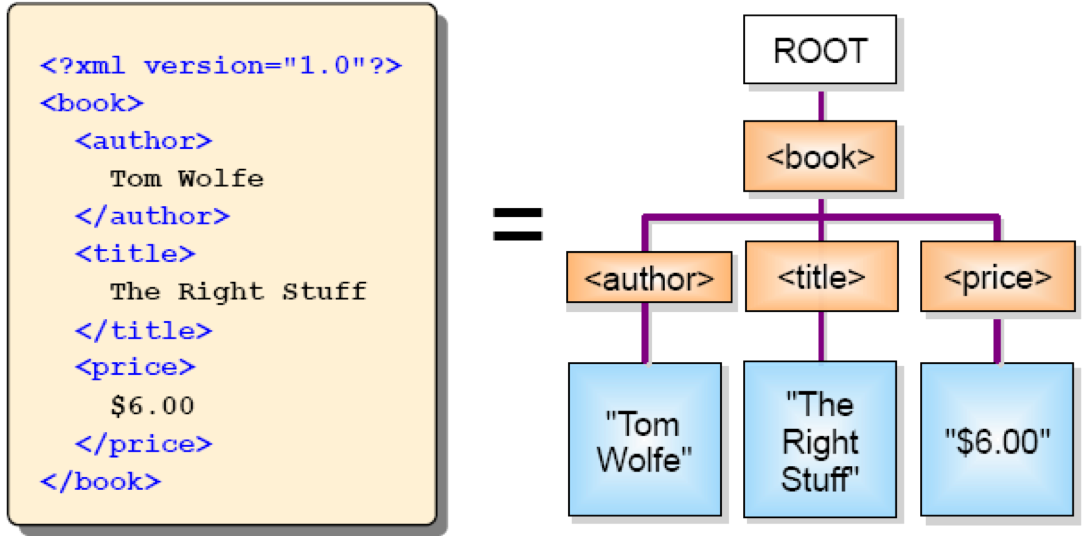
\includegraphics[width=0.7\textwidth]{images/XML文档的树状结构.png}
    \vspace{-1em}
\end{figure}

XML的基本结构:
\begin{figure}[H]
    \vspace{-0.5em}
	\centering
	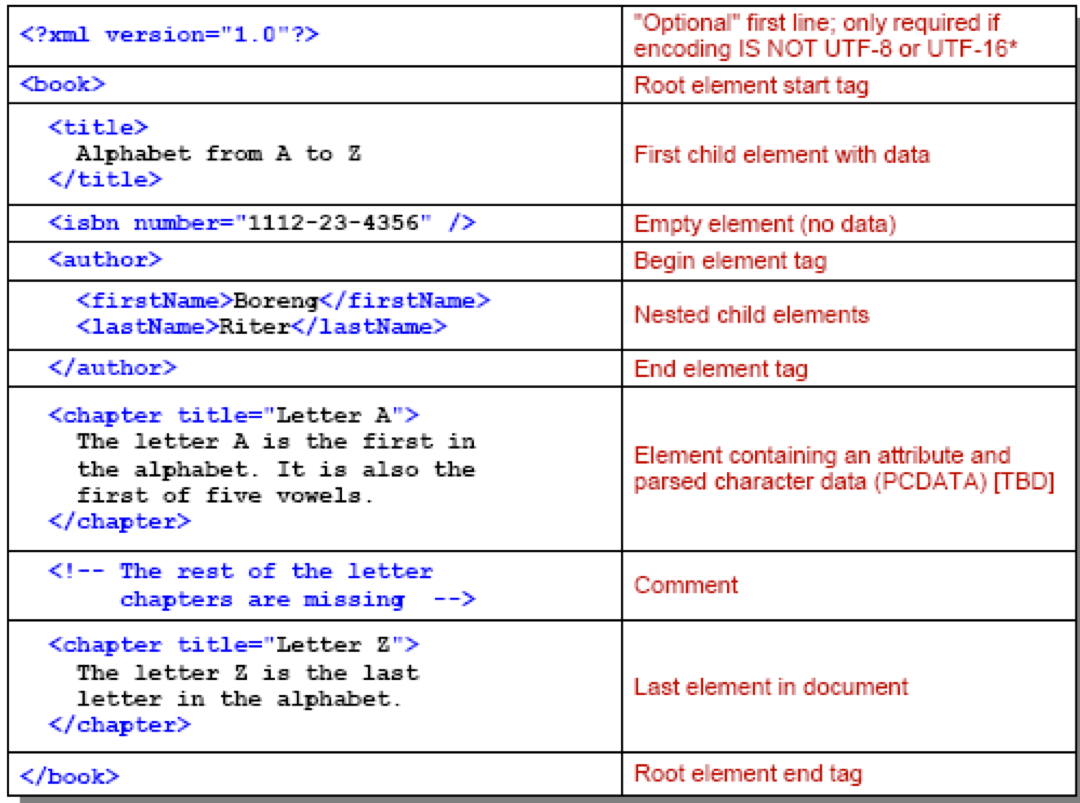
\includegraphics[width=0.7\textwidth]{images/XML的基本结构.png}
    \vspace{-1em}
\end{figure}

\subsubsection{格式良好的XML}
满足$5+1$规则的XML被称为格式良好的XML
\begin{itemize}
    \item 单根元素:所有 XML 文档都只能有一个根元素
    \item 元素标签规则:以开始标签和结束标签来包装元素
    \item 元素嵌套规则:元素标签中间可以嵌套标签
    \item 元素规则
    \begin{itemize}
        \item XML命名:首字母必须是字母或下划线,后街任意长度的字母、数字、连字号等,且不能含有空格,不能以“xml”任何大小写组合作为前缀,XML名称大小写敏感
        \item XML元素内容:XML文档由使用标签对表示的元素、可选属性和可选元素的开始和结束标签之间的数据(可以是文本数据也可以是子元素)所构成。元素内容以两种方式进行处理:
        \begin{itemize}
            \item PCDATA(被解析的字符数据):默认方式,被 XML 解析器进行检查并提取其中的XML内容,这需要对预定义实体进行转义
            \item CDATA(字符数据):采用特殊标记\;\verb|<![CDATA[...]]>|\;进行包装,XML解析器不做处理,只按照字面处理
        \end{itemize}
    \end{itemize}
    \item 元素属性:标签中可以含有属性值键对,用来为元素附加信息,其值必须使用单/双引号括起
    \item XML 声明:可选,出现在 XML 文档中的第一行(\verb|<?xml version="1.0" ?>|,可添加键值对属性)
    \begin{itemize}
        \item encoding属性:用来表达文档所使用的编码,默认为 UTF-8 或 UTF-16
        \item standalone属性:用来表达文档的完整性,即该文档是否依赖于文档外的其他信息,默认为“no”
    \end{itemize}
\end{itemize}


\begin{figure}[H]
	\setcounter{subfigure}{0}
	\centering
	\vspace{-0.5em}	
	\subfloat[单根元素]{
	\begin{minipage}[t]{0.47\linewidth}
	\centering
	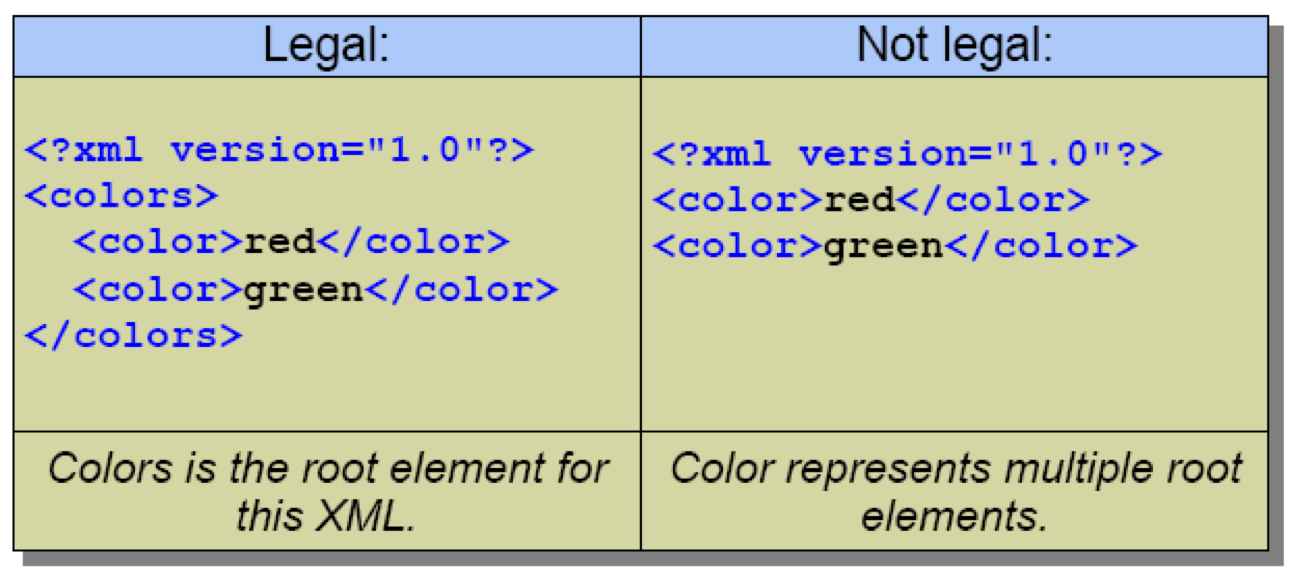
\includegraphics[width=0.97\linewidth]{images/单根元素.png}
	\end{minipage}
	}
    \subfloat[元素嵌套规则]{
	\begin{minipage}[t]{0.47\linewidth}
	\centering
	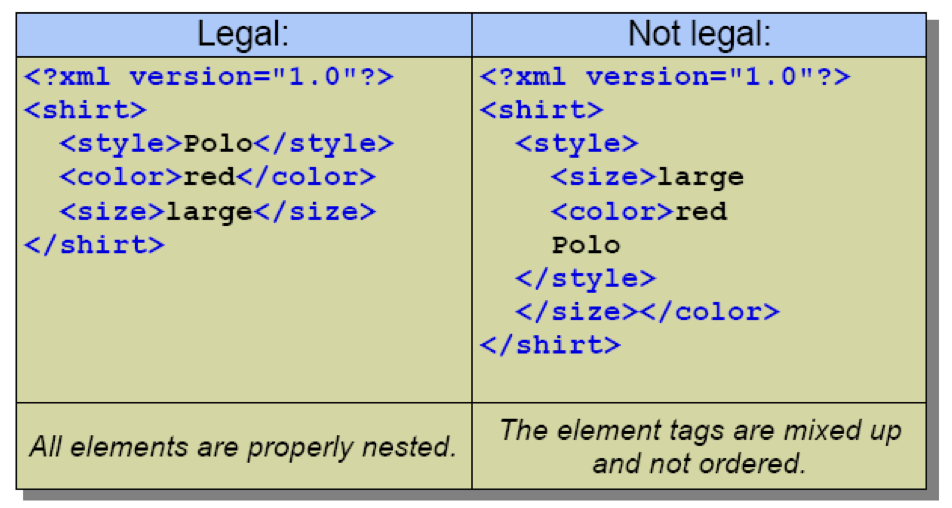
\includegraphics[width=0.93\linewidth]{images/元素嵌套规则.png}
	\end{minipage}
	}
	\centering
	\vspace{-2em}
\end{figure}

\begin{figure}[H]
	\setcounter{subfigure}{2}
	\centering
	\vspace{-0.5em}	
	\subfloat[元素规则:XML命名]{
	\begin{minipage}[t]{0.47\linewidth}
	\centering
	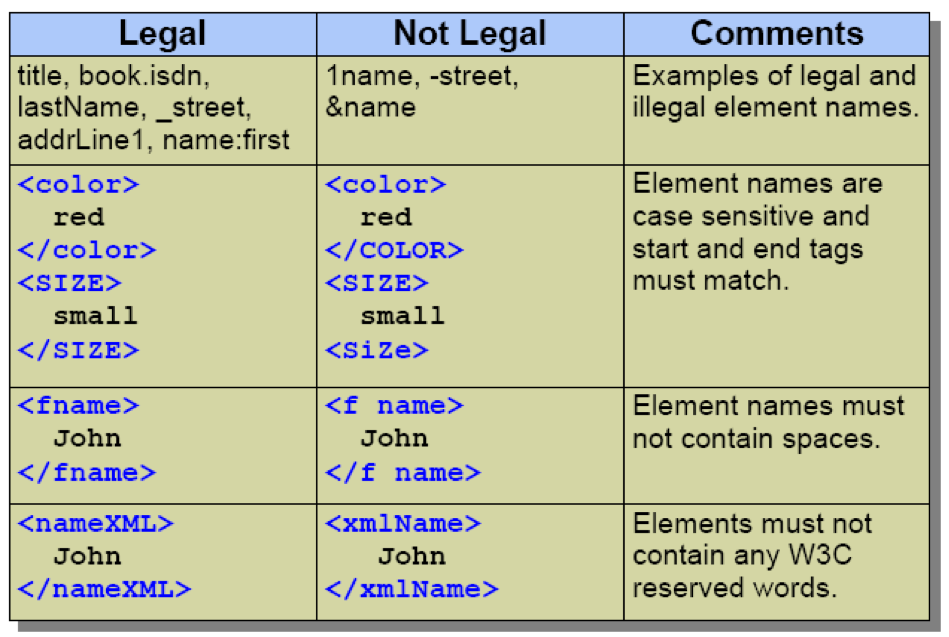
\includegraphics[width=0.97\linewidth]{images/元素规则:XML命名.png}
	\end{minipage}
	}
    \subfloat[元素规则:CDATA]{
	\begin{minipage}[t]{0.47\linewidth}
	\centering
	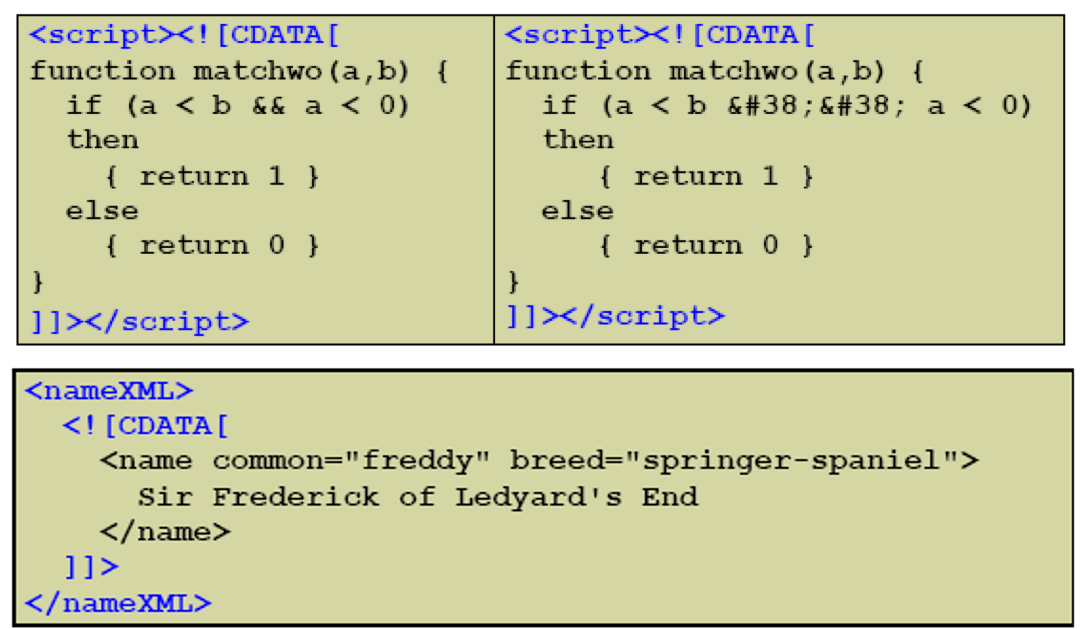
\includegraphics[width=0.97\linewidth]{images/元素规则:CDATA.png}
	\end{minipage}
	}

    \subfloat[元素规则:PCDATA]{
	\begin{minipage}[t]{0.47\linewidth}
	\centering
	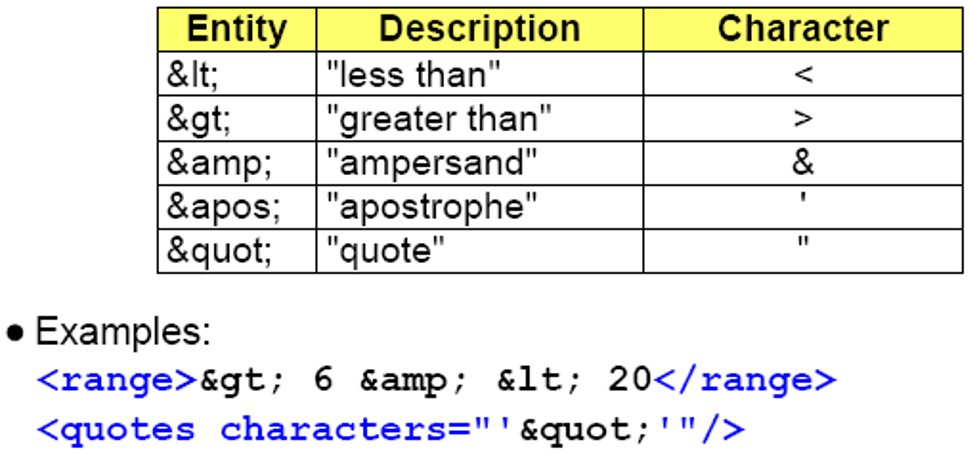
\includegraphics[width=0.97\linewidth]{images/元素规则:PCDATA.png}
	\end{minipage}
	}
    \subfloat[元素属性与XML声明]{
	\begin{minipage}[t]{0.47\linewidth}
	\centering
	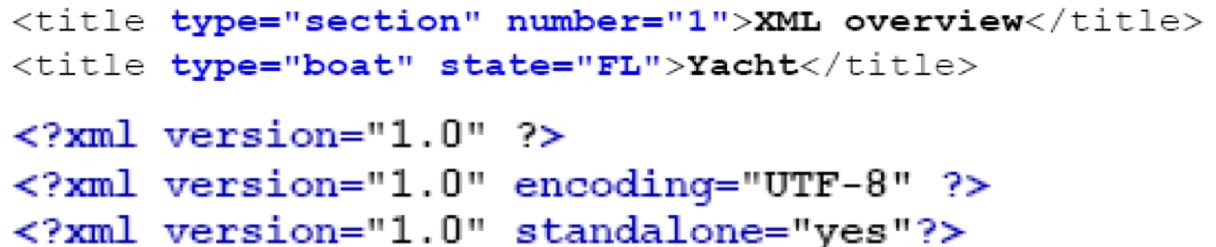
\includegraphics[width=0.97\linewidth]{images/元素属性与XML声明.png}
	\end{minipage}
	}

    \subfloat[注释]{
	\begin{minipage}[t]{0.5\linewidth}
	\centering
	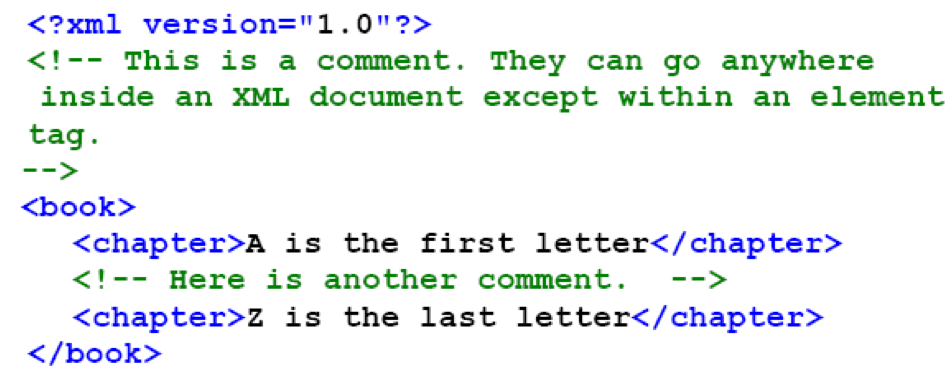
\includegraphics[width=0.97\linewidth]{images/注释.png}
	\end{minipage}
	}
	\centering
	\vspace{-1em}
\end{figure}

一个格式良好的XML文档:
\vspace{-0.8em}
\begin{multicols}{2}
    \begin{itemize}
        \item 由嵌套在另一个XML元素内的XML元素所组成
        \item 具有唯一的根元素
        \item 遵循XML的命名约定
        \item 遵循XML属性引用的规则
        \item 标签被正确终止
    \end{itemize}
\end{multicols}
\vspace{-1em}

所有XML解析器都会检查格式是否良好

有效的XML文档具有一个关联词汇,并遵守该词汇指定的结构规则
\begin{itemize}
    \item 关联词汇通常由DTD或XML Scheme定义
    \item XML解析器可以是验证或非验证的,具体取决于它们是否可以应用关联的语法
    \footnote{XML解析器可以分为两类:验证和非验证。其中,验证解析器可以应用DTD或XML Scheme等关联的语法来验证XML文档是否符合规范。而非验证解析器则不会检查XML文档是否符合规范。换句话说,验证解析器会检查XML文档的语法和结构是否正确,而非验证解析器则只会检查XML文档的格式是否良好。}
\end{itemize}

\subsection{NameSpaces}

\subsubsection{NameSpaces的引入}
NameSpaces的引入:避免在XML文档中出现名称冲突。在XML中,元素和属性都有名称,如果两个不同的元素或属性具有相同的名称,则会导致歧义和混淆。这种冲突的情况在不同的应用程序之间、在不同版本的同一应用程序之间、以及在使用不同的XML词汇表的情况下都可能发生。
\begin{figure}[H]
    \vspace{-0.5em}
	\centering
	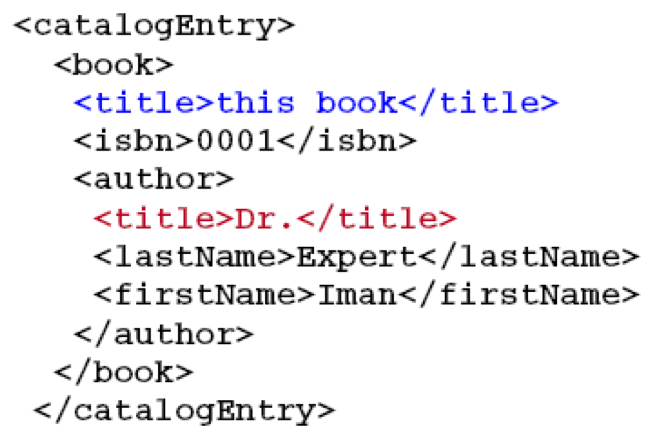
\includegraphics[width=0.38\textwidth]{images/NameSpace的引入.png}
    \vspace{-1em}
\end{figure}

一些可能的解决方案:
\vspace{-0.5em}
\begin{spacing}{1.2}
    \centering
    \begin{longtable}{|m{6cm}<{\centering}|m{8cm}|}
		\hline
		解决方法 & \multicolumn{1}{c|}{说明}  \\ \hline
		采用行业标准的文档格式和命名约定 & 没有哪个行业是孤立的,各行业是相互作用的。这种方法适用于文档级别,一个很好的例子是ebXML,但是元素/属性级别的命名标准过于脆弱 \\ \hline
		使用冗长的元素名称 & 命名变得基本困难,无法知道名称是否已经被使用,而且数据和(或)其模型可能不属于消费应用程序 \\ \hline
		使用一些已经确定为唯一的名称限定符,即域名限定的URI & 域名已经作为唯一标识进行管理和维护。这种方法很有前途,并被发展成为XML命名空间 \\ \hline
    \end{longtable}
	\end{spacing}
\vspace{-1em}

从概念上讲,每个元素名称和属性名称都可以表示为:URI $+$名称,例如\sverb|<title>|\;可能会变成
\begin{lstlisting}
<http://www.library.com/books:title>
\end{lstlisting}
这种格式存在两个问题:
\vspace{-0.8em}
\begin{multicols}{2}
    \begin{itemize}
        \item 它在1.0规范下不是良好格式的XML
        \item 需要输入很多字符
    \end{itemize}
\end{multicols}
\vspace{-1em}

如果能够为URI创建一个同义词,并用该同义词替换URI的出现次数,则输入的字符数量将减少,并且如果处理正确,则结果将与XML 1.0兼容
\begin{itemize}
	\item 例如标记\sverb|books="http://www.library.com/books"|\;然后直接使用 \sverb|<books:title>|
	\item 这个概念形成了XML命名空间规范的基础
\end{itemize}


\subsubsection{QNames}
引入名称空间后,元素名称和属性名称转换为两部分名称,即QNames(Qualified Names)。QNames 用来在 XML 中担任元素名称和属性名称。
\begin{figure}[H]
    \vspace{-0.5em}
	\centering
	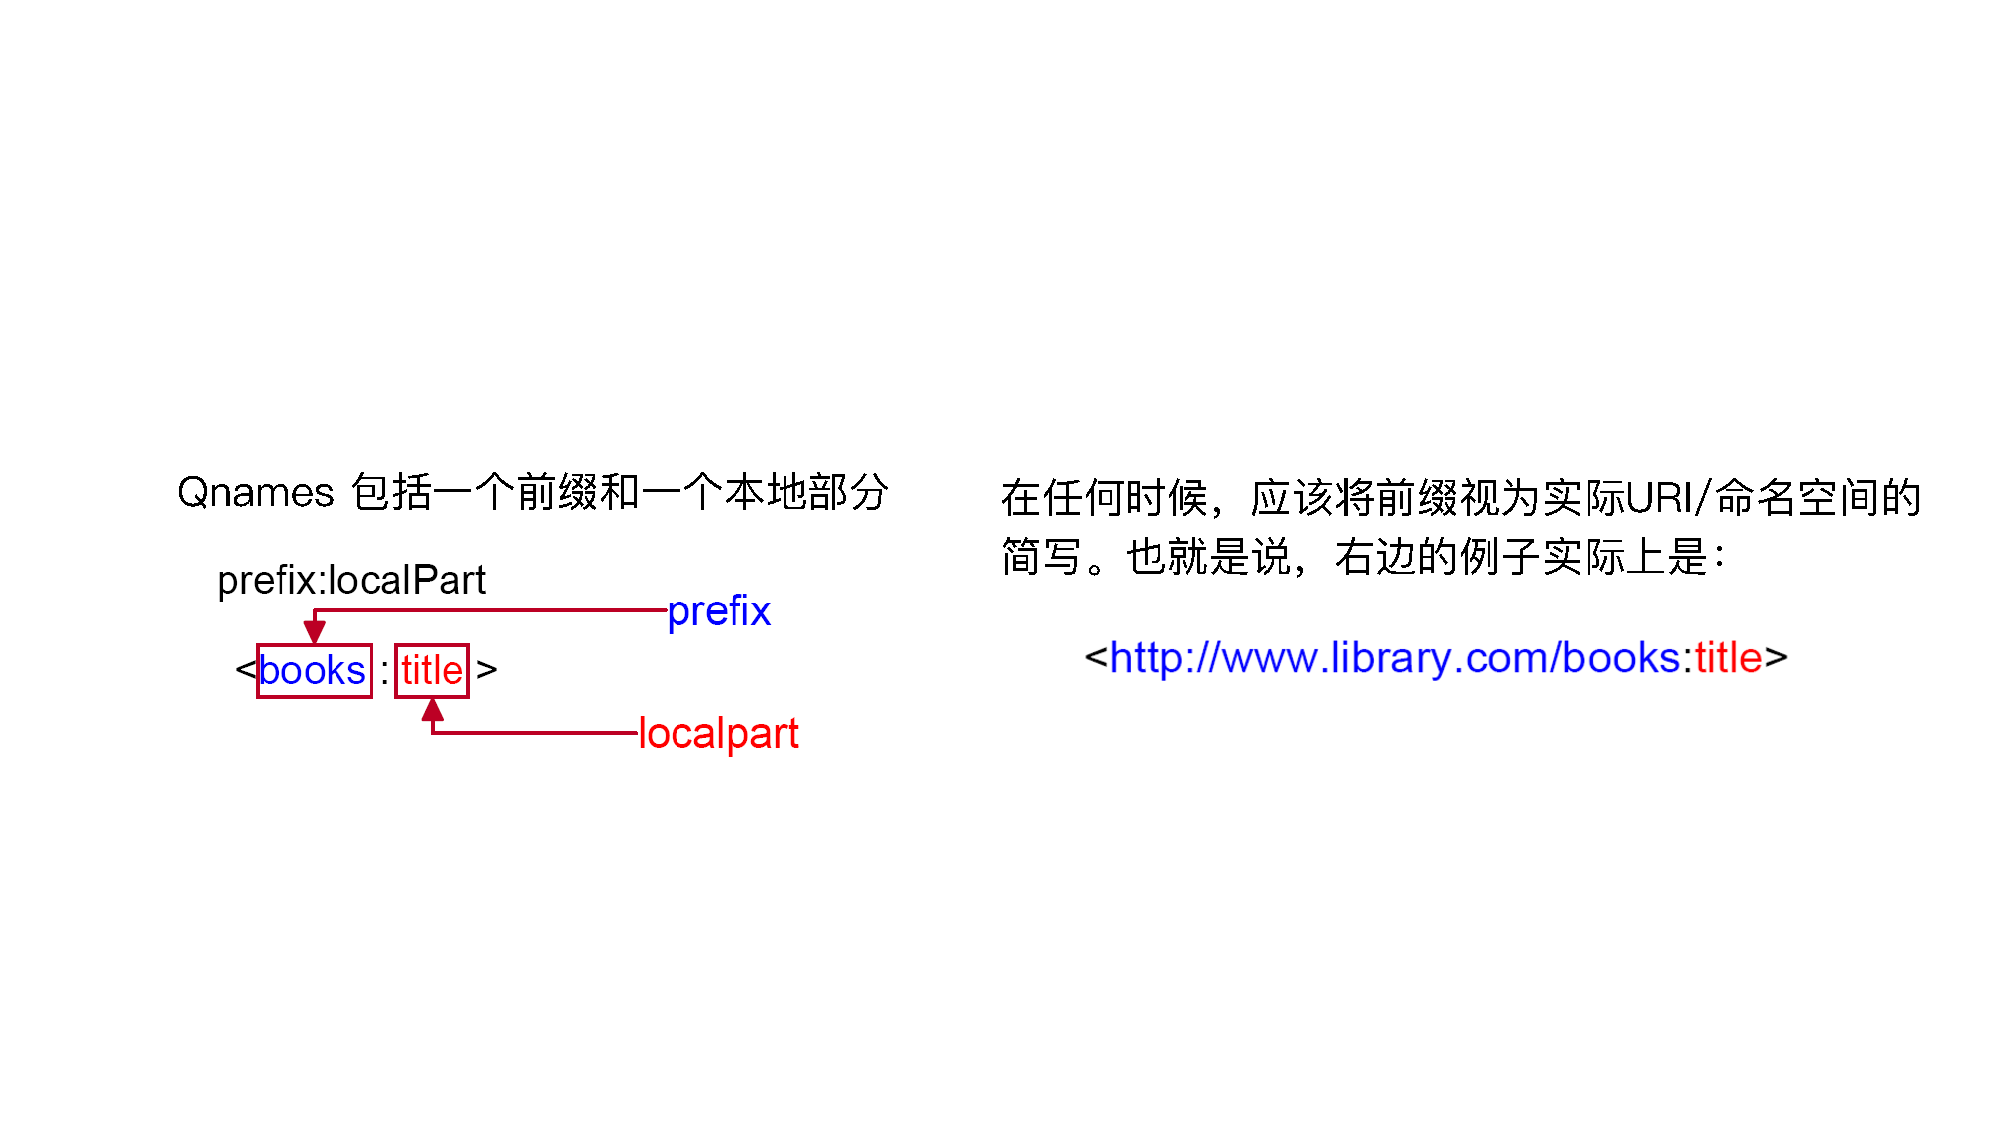
\includegraphics[width=0.95\textwidth]{images/Qnames.pdf}
    \vspace{-1em}
\end{figure}

\subsubsection{Namespaces的声明}
声明Namespaces的语法为
\begin{lstlisting}
<prefix:elementName xmlns:prefix='URI'>
\end{lstlisting}

下面的例子声明了命名空间\;\url{http://www.library.com/books},并将其分配一个前缀为“books”,并将book元素标识为该命名空间的成员
\begin{lstlisting}
<books:book
	xmlns:books='http://www.library.com/books'/>
\end{lstlisting}
属性也可以属于命名空间。与元素一样,属性也要按以下方式加前缀
\begin{lstlisting}
<books:book
	xmlns:books='http://www.library.com/books'
	books:hardcover='true'/>
\end{lstlisting}

\subsubsection{名称空间作用域}
\begin{itemize}
	\item 名称空间前缀的作用域为定义该名称空间的元素(含嵌套的子元素和所隶属的属性)
	\item 名称空间前缀可以在嵌套的子元素中进行重新定义
\end{itemize}

\begin{lstlisting}
<books:book
	xmlns:book='http://www.library.com/books'
	books:hardcover='true'>
		<books:title>
			Tom Sawyer
		</books:title>
</books:book>
\end{lstlisting}

\subsubsection{默认名称空间}
在大多数元素隶属于相同的名称空间时,可以使用默认名称空间
\begin{lstlisting}
<elementName xmlns='URI'/>
\end{lstlisting}
\begin{itemize}
	\item 在默认名称空间的作用域内,可以使用QName来定义隶属于其他名称空间的元素
	\item 默认名称空间不作用于属性,如不使用QName,默认情况下,属性没有名称空间
	\begin{itemize}
		\item 属性隶属于某一个特定的元素,在元素为一确定的情况下,隶属于该元素的拥有不同名称的属性也是唯一确定的
	\end{itemize}
\end{itemize}

\begin{lstlisting}
<book xmlns='http://www.library.com/books'
	xmlns:books='http://www.library.com/books'
	books:hardcover='true'>
  <title>Tom Sawyer</title>
</book>
<!-- book 和 title 隶属于同一个名称空间 -->
\end{lstlisting}

\subsubsection{拥有多个名称空间的XML文档}
\begin{figure}[H]
    \vspace{-0.5em}
	\centering
	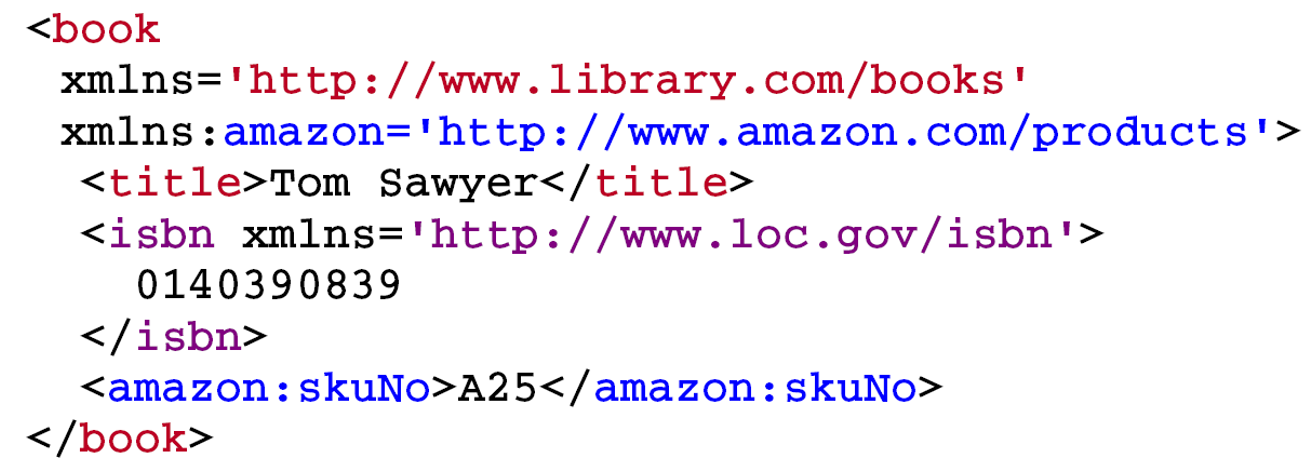
\includegraphics[width=0.7\textwidth]{images/拥有多个名称空间的XML文档}
    \vspace{-1em}
\end{figure}

\subsubsection{没有名称空间的元素}
使用\sverb|xmlns=""|\;用以重置默认名称空间,定义没有名称空间的元素。
\begin{figure}[H]
    \vspace{-0.5em}
	\centering
	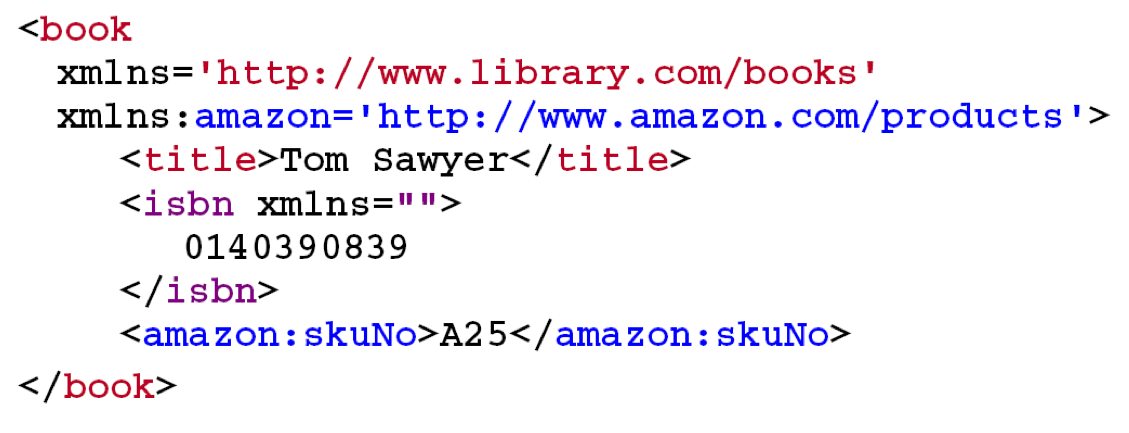
\includegraphics[width=0.65\textwidth]{images/没有名称空间的元素}
    \vspace{-1em}
\end{figure}

\subsubsection{属性与名称空间}
\vspace{-0.8em}
\begin{multicols}{2}
    \begin{itemize}
        \item 属性不受默认命名空间的影响
        \item 特定元素中的属性应各不相同
    \end{itemize}
\end{multicols}
\vspace{-1em}
\begin{figure}[H]
    \vspace{-0.5em}
	\centering
	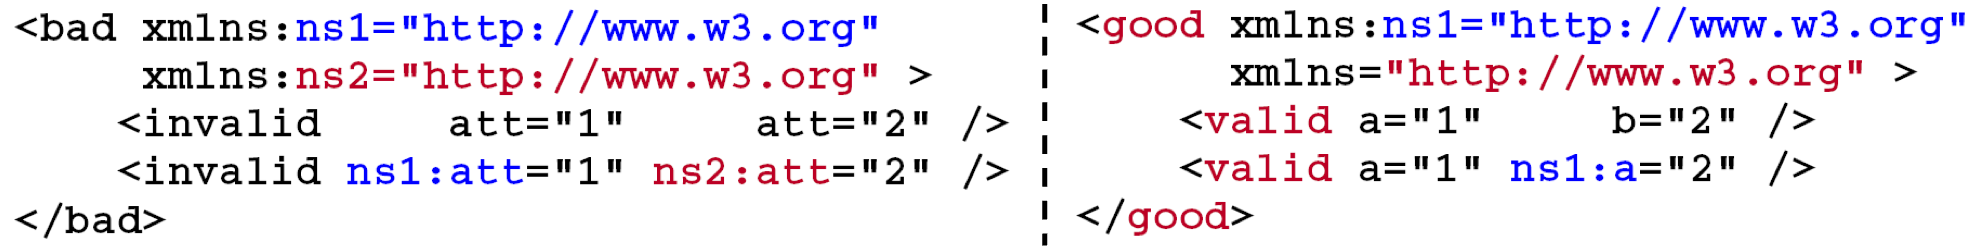
\includegraphics[width=0.96\textwidth]{images/属性与名称空间}
    \vspace{-1em}
\end{figure}

\subsection{XML Schema}

\subsubsection{为什么要引入XML Schema}
从业务角度来看
\vspace{-0.8em}
\begin{multicols}{2}
    \begin{itemize}
        \item 需要增加数据的表示能力
		\item 需要融合来源于不同组织的词汇表
		\item 通过提升通信效率的方式以减少集成的成本
    \end{itemize}
\end{multicols}
\vspace{-1em}

从技术角度来看
\vspace{-0.8em}
\begin{multicols}{2}
    \begin{itemize}
		\item 采用具体的定义验证 XML 文档
		\item 采用 XML 语法
		\item 定义数据结构和约束条件
		\item 支持名称空间
		\item 表达数据元素之间的关系
    \end{itemize}
\end{multicols}
\vspace{-1em}


\subsubsection{XML Schema的结构}
\begin{figure}[H]
    \vspace{-0.5em}
	\centering
	\includegraphics[width=0.7\textwidth]{images/XML Schema的结构.png}
    \vspace{-2em}
\end{figure}


\subsubsection{XML Schema的特点}
\vspace{-0.8em}
\begin{multicols}{2}
	\begin{itemize}
		\item 使用XML实例语法来定义XML文档的结构
		\item 在表达元素和属性内容的数据类型语义方面更加出色
		\item 支持命名空间
		\item 将数据类型的定义与元素和属性的声明分开
		\item 支持表示数据的唯一性和关系
	\end{itemize}
\end{multicols}
\vspace{-1em}


\subsubsection{元素声明}
\paragraph*{定义简单元素}~{} \par
采用已有的类型定义(内建或已定义)来说明元素
\begin{lstlisting}
<xsd:element name='quantity'
			type='xsd:noNegativeInteger'
			minOccurs='1' maxOccurs='1'/>
\end{lstlisting}

其中,name指定元素名称,type指定元素值的类型,minOccurs、maxOccurs指定元素至少、至多出现的次数。类型必须带有命名空间限定符。如果类型未与模式的默认命名空间关联,则必须使用表示正确命名空间的命名空间前缀进行限定。

\textbf{例:}minOccurs与maxOccurs
\begin{figure}[H]
    \vspace{-0.5em}
	\centering
	\includegraphics[width=\textwidth]{images/minOccurs与maxOccurs.png}
    \vspace{-3em}
\end{figure}

\paragraph*{声明子元素}~{} \par
采用排序符定义元素中的子元素
\begin{figure}[H]
    \vspace{-0.5em}
	\centering
	\includegraphics[width=0.75\textwidth]{images/采用排序符定义元素中的子元素}
    \vspace{-1em}
\end{figure}

\textbf{例:}按序列出现的firstName和lastName
\begin{lstlisting}
<xsd:sequence>
 	<xsd:element name='firstName' type='xsd:string'/>
	<xsd:element name='lastName' type='xsd:string'/>
</xsd:sequence>
\end{lstlisting}

\textbf{例:}maidenName和cityOfBirth选择其一
\begin{lstlisting}
<xsd:choice>
	<xsd:element name='maidenName' type='xsd:string'/>
	<xsd:element name='cityOfBirth' type='xsd:string'/>
</xsd:choice>
\end{lstlisting}

\textbf{例:}height和weight以任意顺序出现
\begin{lstlisting}
<xsd:all>
	<xsd:element name='height' type='xsd:float'/>
	<xsd:element name='weight' type='xsd:float'/>
</xsd:all>
\end{lstlisting}

\paragraph*{声明属性}~{} \par
\begin{lstlisting}
<xsd:element name=''>
	<xsd:complexType>
		<xsd:attribute name='attName' type='aSimpleType' fixed|defalut='value' use='...'/>
	</xsd:complexType>
</xsd:element>
\end{lstlisting}
在\sverb|xsd:attribute|\;声明中使用的一些有用(可选)属性包括:
\begin{itemize}
	\item Use:值可以是required(必需的),prohibited(禁止的)和optional(可选的),默认值为optional
	\item Default:当属性不存在时,提供属性的默认值
	\item Fixed:将属性值固定为指定的值
\end{itemize}

对于属性的一些规则:
\vspace{-0.8em}
\begin{multicols}{2}
	\begin{itemize}
		\item 属性类型必须是simpleType(即非元素类型)
		\item \verb|xsd:attribute|\;不能同时存在fixed和default
		\item 当提供默认值时,Use属性必须为“optional”或不存在
	\end{itemize}
\end{multicols}
\vspace{-1em}

\textbf{例:}声明属性
\begin{figure}[H]
    \vspace{-0.5em}
	\centering
	\includegraphics[width=0.98\textwidth]{images/声明属性}
    \vspace{-1em}
\end{figure}

\textbf{例:}同时含有子元素和属性的元素声明
\begin{figure}[H]
    \vspace{-0.5em}
	\centering
	\includegraphics[width=\textwidth]{images/同时含有子元素和属性的元素声明}
    \vspace{-2em}
\end{figure}

\paragraph*{属性组}~{} \par
如果一组属性经常一起使用,则可以创建一个属性组来形式化关系,并避免需要在多个位置声明相同的属性。
\begin{figure}[H]
    \vspace{-0.5em}
	\centering
	\includegraphics[width=\textwidth]{images/属性组}
    \vspace{-2em}
\end{figure}

\subsubsection{XML Schema类型系统}
XML Schema 类型系统分为两个不同的类型类别:简单类型和复杂类型
\vspace{-0.8em}
\begin{multicols}{2}
    \begin{itemize}
		\item 简单类型
		\begin{itemize}
			\item 不能有属性或子元素
			\item 是 XML Schema 类型语言的基本元素
			\item 用于定义其他类型,包括复杂和简单类型
			\item 包括 40 多个预定义的简单类型
		\end{itemize}
		\item 复杂类型
		\begin{itemize}
			\item 可以有属性
			\item 可以用于定义其他复杂类型
			\item 不能用于定义简单类型
			\item 可以有子元素
		\end{itemize}
    \end{itemize}
\end{multicols}
\vspace{-1em}

\paragraph*{取值约束}~{} \par
\begin{figure}[H]
    \vspace{-0.5em}
	\centering
	\includegraphics[width=\textwidth]{images/取值约束}
    \vspace{-2em}
\end{figure}

\paragraph*{枚举约束}~{} \par
\begin{figure}[H]
    \vspace{-0.5em}
	\centering
	\includegraphics[width=0.65\textwidth]{images/枚举约束}
    \vspace{-1em}
\end{figure}

\paragraph*{simpleContent}~{} \par
simpleContent元素必须包含一个restriction或extension元素,这些元素用于定义该元素的简单类型。restriction用于限制元素的取值范围,而extension则用于扩展已有的简单类型。

\begin{lstlisting}
<xsd:complexType name="simpleContentType">
	<xsd:simpleContent>
		<xsd:extension base="xsd:...">
		...
		</xsd:extension>
	</xsd:simpleContent>
</xsd:complexType>
\end{lstlisting}

\begin{figure}[H]
    \vspace{-0.5em}
	\centering
	\includegraphics[width=0.75\textwidth]{images/枚举约束}
    \vspace{-1em}
\end{figure}

\paragraph*{element only}~{} \par
当一个类型被声明为element only,就指定该类型的实例只能包含元素,而不能包含文本或字符数据。也就是说,该类型的实例不允许出现文本节点或CDATA节点,只能是元素节点。
\begin{lstlisting}
<xsd:complexType name="elementOnlyType">
	<xsd:sequence>
		<xsd:element name="firstName" type="xsd:string"/>
		<xsd:element name="lastName" type="xsd:string"/>
	</xsd:sequence>
<xsd:complexType>
\end{lstlisting}

\paragraph*{Mixed}~{} \par
当一个类型被声明为mixed,它指定该类型的实例可以包含元素、文本或字符数据,或它们的任意组合。也就是说,该类型的实例允许同时包含元素节点和文本节点或CDATA节点。
\begin{lstlisting}
<xsd:complexType name=mixedType" mnixed=true">
	<xsd:sequence>
		<xsd:element name="firstName" type="xsd:string"/>
		<xsd:element name="lastName" type="xsd:string"/>
</xsd:sequence>
</xsd:complexType>
\end{lstlisting}

\paragraph*{具名类型与匿名类型}~{} \par
\begin{itemize}
	\item 在XML Schema中,一个元素可以有一个具名类型或一个匿名类型。具名类型是通过名称来引用的,而匿名类型是定义元素时内联定义的类型。
	\item 具名类型是为多个元素定义的,可以被引用并重复使用,而匿名类型仅用于单个元素。具名类型可以在文档中的多个地方重复使用,而匿名类型只能在定义它们的元素上使用。
	\item 具名类型可以提高XML Schema的可重用性和可维护性,而匿名类型则可以减少模式定义时的冗余。
\end{itemize}

\begin{figure}[H]
	\setcounter{subfigure}{0}
	\centering
	\vspace{-1.5em}	
	\subfloat[具名类型]{
	\begin{minipage}[t]{0.41\linewidth}
	\centering
	\includegraphics[width=0.97\linewidth]{images/具名类型.png}
	\end{minipage}
	}
    \subfloat[匿名类型]{
	\begin{minipage}[t]{0.53\linewidth}
	\centering
	\includegraphics[width=0.97\linewidth]{images/匿名类型.png}
	\end{minipage}
	}
	\centering
	\vspace{-1em}
\end{figure}

匿名类型也可以用在属性声明中
\begin{figure}[H]
    \vspace{-0.5em}
	\centering
	\includegraphics[width=0.85\textwidth]{images/属性声明中的匿名类型.png}
    \vspace{-2.5em}
\end{figure}

\paragraph*{全局类型与局部类型}~{} \par
\begin{itemize}
	\item 类型可以在元素中声明为局部类型。匿名类型是局部类型。
	\item 类型可以在模式元素的直接子级中全局声明。命名类型是全局类型。
	\item 只有顶级类型可以命名和重复使用。
\end{itemize}

\begin{figure}[H]
    \vspace{-0.5em}
	\centering
	\includegraphics[width=0.65\textwidth]{images/全局声明.png}
    \vspace{-1em}
\end{figure}

\subsubsection{在XML中说明名称空间}
\begin{lstlisting}
<xsd:schema
	xmlns="http://www.ibm.com/schemas/WD03/target"
	xmlns:xsd="http://www.w3.org/2001/XMLSchema"
	targetNamespace="http://www.ibm.com/Schemas/WD03/target" elementFormDefault="qualified">
	<xsd:element name="quantity" type="xsd:integer"/>
</xsd:schema>
\end{lstlisting}
在schema脚本中所定义的元素,理论上来说都应该被放置或关联到一个特定的名称空间
\begin{itemize}
	\item targetNamespace中的URI就是当前这个schema脚本中所定义的元素(在上例中为quantity)隶属的名称空间
\end{itemize}


\subsubsection{寻找XML Schema}
\begin{figure}[H]
	\setcounter{subfigure}{0}
	\centering
	\vspace{-1.5em}	
	\subfloat{
	\begin{minipage}[c]{0.47\linewidth}
	\centering
	\includegraphics[width=0.97\linewidth]{images/寻找XML Schema.png}
	\end{minipage}
	}
    \subfloat{
	\begin{minipage}[c]{0.47\linewidth}
	\centering
	\includegraphics[width=0.97\linewidth]{images/寻找XML Schema2.png}
	\end{minipage}
	}
	\centering
	\vspace{-1em}
\end{figure}

使用XML Schema Instance(xsi)用于指定 XML 实例文档与 XML Schema 之间关联的命名空间前缀。它是由 XML Schema 规范定义的,用于表示 XML 实例文档中使用的元素和属性是基于哪个 XML Schema 定义的。

通过在 XML 实例文档中使用该命名空间前缀和schemaLocation属性,可以指定 XML Schema 文件的位置和名称,从而使 XML 解析器能够在验证 XML 实例文档时使用正确的 XML Schema 文件。

\textbf{例:}下面的 XML 实例文档中使用了xsi命名空间前缀,并使用schemaLocation属性指定了XML Schema文件的位置:
\begin{lstlisting}
<?xml version="1.0" encoding="UTF-8"?>
<root xmlns:xsi="http://www.w3.org/2001/XMLSchema-instance"
      xsi:schemaLocation="http://www.example.com/schema/schema.xsd">
  <element1>value1</element1>
  <element2>value2</element2>
</root>
\end{lstlisting}

	\section{服务模型}

\subsection{SOAP}

\subsubsection{SOAP的引入}
\begin{itemize}
    \item 现在我们有:
    \begin{itemize}
        \item 我们使用XML定义了Web Service中的消息交换格式
        \item 通过引入NameSpace使得XML中的元素(Element)/属性(Attribute)全球唯一且全球共享
        \item 通过Schema定义了数据类型(同上)
    \end{itemize}
    \item 下一个问题是:使用Web Service作为服务的具体实现技术,服务的发布/查找、调用,都需要通过互联网传递XML消息
    \begin{itemize}
        \item 一个可能的方法是,直接将XML作为文本载荷通过特定网络协议(HTTP,SMTP,FTP等)加以传递
        \item 为什么选择SOAP:提供了一种标准的方法,使得运行在不同平台并使用不同的技术和编程语言的应用程序可以互相进行通信
    \end{itemize}   
\end{itemize}

\subsubsection{什么是SOAP}
SOAP提供了一种标准的方法,使得运行在不同平台并使用不同的技术和编程语言的应用程序可以互相进行 XML 通信。从本质上来说,SOAP并不是一个网络传输协议,它仅仅是一个信息传递的概念性框架,在实际使用时,需要绑定具体的网络传输协议和上层的应用逻辑来创建关联。
\begin{itemize}
    \item SOAP使用XML定义了可扩展的消息架构,该消息架构提供了能够基于多种底层协议,进行信息交换的信息架构。
    \item SOAP基本上是一种无状态的单向消息交换范例。应用程序可以通过将这种单向交换与底层协议提供的功能和/或应用程序特定信息相结合来创建更复杂的交互模式(例如,请求/响应、请求/多个响应等)。
    \item SOAP提供在可扩展的方式下传递应用程序特定信息的框架和接收SOAP消息时SOAP节点执行的所有必需操作的完整描述。
    \item SOAP并不关心它所携带的应用相关数据的语义(就像信封不关心在信封中装的是支票还是邮件)、SOAP消息路由、可靠数据传输、防火墙穿越等问题。
\end{itemize}

\subsubsection{SOAP的两种使用方式}
\begin{figure}[H]
	\setcounter{subfigure}{0}
	\centering
	\vspace{-2em}	
	\subfloat[没有中间转发节点]{
	\begin{minipage}[t]{0.3\linewidth}
	\centering
	\includegraphics[width=0.97\linewidth]{images/SOAP没有中间转发节点.pdf}
	\end{minipage}
	}
    \subfloat[有多个中间转发节点]{
	\begin{minipage}[t]{0.66\linewidth}
	\centering
	\includegraphics[width=0.93\linewidth]{images/SOAP有多个中间转发节点.pdf}
	\end{minipage}
	}
	\centering
	\vspace{-1.5em}
\end{figure}


\subsubsection{SOAP的两种交互模式}
RPC(远程过程调用)模式:
\vspace{-0.3em}
\begin{multicols}{2}
    \begin{itemize}
        \item 同步的请求/应答交互模式
        \item 发送请求并等待响应
    \end{itemize}
\end{multicols}
\vspace{-1em}

面向文档模式(大多数情况):
\begin{vwcol}[widths={0.3\textwidth,0.65\textwidth},rule=0pt]
    \hspace{1em}{\footnotesize$\bullet$}\hspace{0.5em}异步交互模式

    {\footnotesize$\bullet$}\hspace{0.5em}发送复杂的XML文档,并等待通知,结果会在处理后发回
\end{vwcol}


\subsubsection{SOAP结构}
\begin{figure}[H]
    \vspace{-0.5em}
	\centering
	\includegraphics[width=0.7\textwidth]{images/SOAP结构.pdf}
    \vspace{-1em}
\end{figure}

\paragraph*{SOAP消息示例}~{} \par
\begin{figure}[H]
    \vspace{-0.5em}
	\centering
	\includegraphics[width=\textwidth]{images/SOAP Messages Example.pdf}
    \vspace{-3em}
\end{figure}

\paragraph*{远程过程调用(RPC)}~{} \par
\begin{figure}[H]
    \vspace{-0.5em}
	\centering
	\includegraphics[width=0.67\textwidth]{images/Remote Procedure Calls.pdf}
    \vspace{-2em}
\end{figure}

RPC应答1
\begin{figure}[H]
    \vspace{-0.5em}
	\centering
	\includegraphics[width=0.75\textwidth]{images/RPC1.pdf}
    \vspace{-1em}
\end{figure}

RPC应答2
\begin{figure}[H]
    \vspace{-0.5em}
	\centering
	\includegraphics[width=0.7\textwidth]{images/RPC2.pdf}
    \vspace{-1em}
\end{figure}

\paragraph*{出错场景}~{} \par
\begin{figure}[H]
    \vspace{-0.5em}
	\centering
	\includegraphics[width=0.75\textwidth]{images/Fault Scenarios.pdf}
    \vspace{-3em}
\end{figure}

\paragraph*{SOAP绑定}~{} \par
在抽象的消息交互框架中,SOAP消息需要使用底层协议完成传输,如何使用底层协议完成 OAP消息的封装、处理和传输,由SOAP绑定进行定义。

最常见的SOAP绑定是HTTP绑定,该绑定使用Web方法(GET和POST),采用HTTP消息交互的方式,支持SOAP消息传递。

此外,它还使用两种消息交换模式(MEP, message exchange patterns),提供了两种通过HTTP交换SOAP消息的方法:
\begin{itemize}
    \item 一种是使用HTTP POST方法在HTTP请求和响应消息的正文中传递SOAP消息,这种方法使用了一个称为SOAP请求-响应MEP的功能
    \item 另一种是使用HTTP GET方法在HTTP请求中返回一个包含SOAP消息的HTTP响应的正文,这种方法使用了一个称为SOAP响应MEP的功能
\end{itemize}

SOAP HTTP POST
\begin{figure}[H]
    \vspace{-0.5em}
	\centering
	\includegraphics[width=\textwidth]{images/SOAP绑定POST.pdf}
    \vspace{-3em}
\end{figure}

SOAP HTTP GET
\begin{figure}[H]
    \vspace{-0.5em}
	\centering
	\includegraphics[width=0.8\textwidth]{images/SOAP绑定get.pdf}
    \vspace{-1.5em}
\end{figure}

除了HTTP绑定,其他绑定还可以有SMTP、HTTPS、MIME等

\subsection{WSDL}

\subsubsection{WSDL的引入}
\begin{itemize}
    \item 现在我们有:
    \begin{itemize}
        \item XML,Namespace,XML Schema完成消息格式和数据结构定义
        \item SOAP作为传递XML消息的传输协议(最简)
    \end{itemize}
    \item 下一个问题是:我们怎么知道,在什么地方/以什么方式/能够调用到什么样的Web Service?
    \begin{itemize}
        \item 一个可能的方法是,Out-of-band(例如完成了一个Web Service开发后通过邮件告诉相应的人有关信息或直接提供相关说明文档)
        \item 为什么使用WSDL:提供了一种基于XML的标准接口定义语言/服务能力定义语言,用以在服务的提供者/调用者/服务注册之间,交换必要的有关Web Service 的信息
        \item WSDL是否携带了关于Web Service的足够信息?可能是也可能否,取决于Web Service本身的复杂性和业务特性
    \end{itemize}
\end{itemize}

\subsubsection{WSDL模型的基本概念}
WSDL是用以描述网络服务的XML格式,它将服务描述为基于消息(面向文档/面向过程)运作的端点(endpoints)集合。通常WSDL、SOAP 和 XML Schema 会被同时使用。
\vspace{-0.5em}
\begin{spacing}{1.2}
    \begin{longtable}{|m{4cm}|m{9cm}|}
        \hline
        \multicolumn{1}{|c|}{WSDL回答了}  &  \multicolumn{1}{c|}{WSDL提供了}\\ \hline
        \vspace{-1.3em}
        \begin{itemize}[leftmargin=1.5em,itemsep=-2pt]
            \item 服务用来干什么
            \item 服务在哪
            \item 如何调用服务
            \vspace{-1.5em}
        \end{itemize} &  
        \vspace{-1.3em}
        \begin{itemize}[leftmargin=1.5em,itemsep=-2pt]
            \item 功能信息
            \item 消息结构(如何说明消息交互中的数据类型)
            \item 协议绑定(如何将抽象消息映射为具体的网络传输)
            \vspace{-1.5em}
        \end{itemize}
        \\\hline
    \end{longtable}
\end{spacing}
\vspace{-1em}

WSDL的历史
\begin{itemize}
    \item WSDL 1.0(2000年9月)由IBM,Microsoft和Ariba开发,用于描述其SOAP工具包的Web服务。它是通过将IBM的NASSL(网络应用程序服务规范语言)和Microsoft的SDL(服务描述语言)两种服务描述语言结合而构建的。
    \item WSDL 1.1于2001年3月发布,是对WSDL 1.0的正式规范化。在1.0和1.1间没有引入重大变化。
    \item WSDL 1.2(2003年6月)是W3C的工作草案,后因与WSDL 1.1有重大差异更名为WSDL 2.0。
    \begin{itemize}
        \item 根据W3C的说法,WSDL 1.2比以前的版本更易于开发人员使用和更加灵活。WSDL 1.2试图删除不可互操作的特性,并更好地定义了HTTP 1.1绑定。
        \item 大多数SOAP服务器/供应商不支持WSDL 1.2。
    \end{itemize}
    \item WSDL 2.0于2007年6月成为W3C推荐标准。
\end{itemize}

\subsubsection{WSDL 2.0信息集结构}
\begin{figure}[H]
    \vspace{-1em}
	\centering
	\includegraphics[width=0.6\textwidth]{images/WSDL 2.0信息集结构.png}
    \vspace{-2.5em}
\end{figure}

\begin{itemize}
    \item import、include:主要用来对于撰写在多个文档中间的 WSDL 信息进行拼接,前者用于从不同的名称空间引入,后者用于从相同的名称空间引入
    \item types:用来说明消息结构
    \item interface:用来指定抽象意义下服务所提供的能力的相关接口
    \item binding:用来将 inerface 指定的抽象的消息格式转为具体的消息格式
    \item service:通过聚合 endpoint 在 interface 和 binding 之间来创建映射关系
\end{itemize}

\subsubsection{WSDL 2.0的语法和机制}
\paragraph*{定义声明和名称空间}~{} \par
\begin{figure}[H]
    \vspace{-0.5em}
	\centering
	\includegraphics[width=0.65\textwidth]{images/定义声明和名称空间.pdf}
    \vspace{-1.5em}
\end{figure}

\paragraph*{定义消息类型types}~{} \par
\begin{figure}[H]
    \vspace{-0.5em}
	\centering
	\includegraphics[width=\textwidth]{images/定义消息类型.pdf}
    \vspace{-3em}
\end{figure}

\paragraph*{定义接口interface}~{} \par
\begin{figure}[H]
	\setcounter{subfigure}{0}
	\centering
	\vspace{-1.5em}	
	\subfloat[定义接口interface]{
	\begin{minipage}[t]{0.66\linewidth}
	\centering
	\includegraphics[width=\linewidth]{images/定义接口.pdf}
	\end{minipage}
	}
	\subfloat[4种基本的MEP,若每一种再加上出错处理,就得到另外4种]{
	\begin{minipage}[t]{0.31\linewidth}
	\centering
	\includegraphics[width=\linewidth]{images/4种基本MEP.png}
	\end{minipage}
	}
	\centering
	\vspace{-4em}
\end{figure}

\paragraph*{定义绑定binding}~{} \par
\begin{figure}[H]
    \vspace{-0.7em}
	\centering
	\includegraphics[width=0.87\textwidth]{images/定义绑定binding.pdf}
    \vspace{-1.5em}
\end{figure}

\paragraph*{定义服务service}~{} \par
\begin{figure}[H]
    \vspace{-0.7em}
	\centering
	\includegraphics[width=0.93\textwidth]{images/定义服务service.pdf}
    \vspace{-1.5em}
\end{figure}

\paragraph*{文档化服务}~{} \par
\begin{figure}[H]
    \vspace{-0.7em}
	\centering
	\includegraphics[width=0.83\textwidth]{images/文档化服务.pdf}
    \vspace{-1.5em}
\end{figure}

\paragraph*{RPC风格}~{} \par
\begin{figure}[H]
    \vspace{-0.7em}
	\centering
	\includegraphics[width=\textwidth]{images/RPC风格.pdf}
    \vspace{-1.5em}
\end{figure}

\subsubsection{WSDL简化结构}
\begin{figure}[H]
    \vspace{-0.7em}
	\centering
	\includegraphics[width=0.75\textwidth]{images/WSDL简化结构.pdf}
    \vspace{-1em}
\end{figure}

\begin{figure}[H]
    \vspace{-0.7em}
	\centering
	\includegraphics[width=0.9\textwidth]{images/服务簇.pdf}
    \vspace{-1em}
\end{figure}

\subsubsection{WSDL 1.1与WSDL 2.0的差异}
一方面是一些名称上的差异(portType和interface、port和endpoint);另一方面在WSDL 1.1中有一个单独用来说明中继消息message的element,而WSDL 2.0中没有。
\begin{figure}[H]
    \vspace{-0.7em}
	\centering
	\includegraphics[width=0.55\textwidth]{images/WSDL 1.1与WSDL 2.0的差异.png}
    \vspace{-1em}
\end{figure}

\subsection{BPEL}

\subsubsection{BPEL的引入}
\begin{itemize}
    \item 现在我们有:
    \vspace{-0.8em}
    \begin{multicols}{2}
        \begin{itemize}
            \item XML,Namespace,XML Schema,SOAP
            \item WSDL用来定义服务/服务能力
        \end{itemize}
    \end{multicols}
    \vspace{-1em}
    \item 下一个问题是:为了建模服务,XML,SOAP,WSDL是不是足够了?
    \begin{itemize}
        \item 一个可能的答案,是的
        \item 另一个可能,对于更加复杂的服务,仍然不够
        \vspace{-1.2em}
        \begin{multicols}{2}
            \begin{itemize}
                \item 一个复合服务(WS-BPEL,WS-CDL)
                \item 一个带非功能性需求的服务(WS-*)
                \item 服务提供方和服务调用方之间交换信息的其他方法
            \end{itemize}
        \end{multicols}
        \vspace{-1em}
    \end{itemize}
\end{itemize}

\subsubsection{复合服务}
为什么需要复合服务:复用和灵活
\begin{itemize}
    \item 有些服务是垂直的,有些服务是水平的。为保证复用性,某些垂直服务被设计为由水平服务构造而来
    \item 如果活动由服务实现,那么由活动构成的(商业)流程由复合服务实现
\end{itemize}

如何实现复合服务:
\begin{itemize}
    \item 一个可能的方法,在传统编程环境中,调用子服务,再把编程单元封装成服务以供调用
    \item 采用标准协议的XML脚本描述服务组合方式
\end{itemize}

建模复合Web服务:要建模一个涉及多个参与方的业务流程,可能需要多个Web服务协作来形成一个复合Web服务,它们在逻辑上是独立的,可能由不同的提供者实现。

\subsubsection{BPEL的概念}
业务流程执行语言(Business Process Execution Language, BPEL4WS、WS4BPEL、BPEL或WS-BPEL)是一种用于协调Web服务以实现全面业务流程的流程表示方式。BPEL是一种基于XML的,用来描写业务过程的编程语言,被描写的业务过程的每个单一步骤则由Web服务来实现。
\begin{itemize}
    \item 定义了一种互操作的集成模型,以促进自动化流程集成在企业内部和企业之间环境中的扩展。
    \item BPEL流程定义了如何协调多个业务交互以实现共同的业务目标,并具有必要的状态和逻辑来进行协调。
    \item 精确定义了跨企业业务协议的基本服务行为,例如:
    \vspace{-0.8em}
    \begin{multicols}{3}
        \begin{itemize}
            \item 数据相关行为
            \item 异常情况及其后果
            \item 各粒度的长时间运行交互
        \end{itemize}
    \end{multicols}
    \vspace{-1em}
    \item 将业务流程的公共行为与其内部实现分离开来。
    \item 有两种方式可以对业务流程进行建模:
    \begin{itemize}
        \item 可执行的流程模型:模拟业务交互参与方的实际行为
        \item 抽象模型:指定涉及方的互相可见的消息交换行为,而不揭示它们的内部行为
    \end{itemize}
    \item 在BPEL中创建业务流程的两个步骤:
    \vspace{-0.8em}
    \begin{multicols}{2}
        \begin{itemize}
            \item 创建服务描述
            \item 创建业务流程
        \end{itemize}
    \end{multicols}
    \vspace{-1em}
\end{itemize}

\subsubsection{一个简单的复合Web Service}
\begin{figure}[H]
    \vspace{-0.7em}
	\centering
	\includegraphics[width=0.92\textwidth]{images/一个简单的复合Web Service.pdf}
    \vspace{-1.5em}
\end{figure}

\subsubsection{BPEL应用实例}
\paragraph*{创建服务描述}~{} \par
使用 WSDL 定义相关方和消息(用于支付和运输提供商Shipping/Payment Service Providers)
\begin{figure}[H]
    \vspace{-0.7em}
	\centering
	\includegraphics[width=0.95\textwidth]{images/创建服务描述.pdf}
    \vspace{-1.5em}
\end{figure}

使用WSDL定义供应商Suppliers
\begin{figure}[H]
    \vspace{-0.7em}
	\centering
	\includegraphics[width=\textwidth]{images/创建服务描述2.pdf}
    \vspace{-5.5em}
\end{figure}

\paragraph*{创建业务过程}~{} \par
可以使用端口类型、操作和消息类型的定义来详细说明流程
\begin{figure}[H]
    \vspace{-0.5em}
	\centering
	\includegraphics[width=0.7\textwidth]{images/创建业务过程.pdf}
    \vspace{-1em}
\end{figure}

\begin{figure}[H]
    \vspace{-0.5em}
	\centering
	\includegraphics[width=\textwidth]{images/创建业务过程2.pdf}
    \vspace{-3em}
\end{figure}

\subsubsection{BPEL关键元素}

\vspace{-0.5em}
\begin{spacing}{1.2}
    \centering
    \begin{longtable}{|m{3.7cm}<{\centering}|m{11cm}|}
    \hline
    \textbf{element} & \multicolumn{1}{c|}{\textbf{描述}} \\ \hline
    partners &
    \vspace{-1.3em}
    \begin{itemize}[leftmargin=1.5em,itemsep=-2pt]
        \item 定义正在构建的业务流程与其合作流程之间的关系
        \item 合作伙伴可以作为
        \vspace{-0.2em}
        \begin{itemize}[leftmargin=1.5em,itemsep=-2pt]
            \item 提供业务流程所使用的服务的消费者
            \item 提供被业务流程使用的服务的提供者
            \item 激活业务流程的服务
        \end{itemize}
    \vspace{-1.5em}
    \end{itemize}                                           
    \\ \hline
    partner link types &
    \vspace{-1.3em}
    \begin{itemize}[leftmargin=1.5em,itemsep=-2pt]
        \item 定义两个Web服务之间的对话关系
        \item 在WSDL中定义,并给出与portType相关联的角色
    \vspace{-1.5em}
    \end{itemize}                                           
    \\ \hline
    partner links &
    \vspace{-1.3em}
    \begin{itemize}[leftmargin=1.5em,itemsep=-2pt]
        \item 对业务流程与其交互的合作伙伴服务进行建模
        \item 由partner link type所特征化
        \item 定义业务流程内的静态关系
    \vspace{-1.5em}
    \end{itemize}                                           
    \\ \hline
    business partners &
    \vspace{-1.3em}
    \begin{itemize}[leftmargin=1.5em,itemsep=-2pt]
        \item 使用partner元素对需要多个对话关系的业务合作伙伴关系进行建模
        \item 允许对partner links进行分组
        \item 禁止重叠
    \vspace{-1.5em}
    \end{itemize}                                           
    \\ \hline
    endpoint references &
    \vspace{-1.3em}
    \begin{itemize}[leftmargin=1.5em,itemsep=-2pt]
        \item 为服务提供端口特定数据提供动态绑定机制
        \item 允许将服务提供者与partner links中的角色进行动态绑定
    \vspace{-1.5em}
    \end{itemize}                                           
    \\ \hline
    activities &
    \vspace{-1.3em}
    \begin{itemize}[leftmargin=1.5em,itemsep=-2pt]
        \item 基本活动,例如接收、回复和调用
        \item 结构化活动
        \vspace{-0.2em}
        \begin{itemize}[leftmargin=1.5em,itemsep=-2pt]
            \item 按顺序执行(序列、开关和循环)
            \item 并发执行(流程)
            \item 非确定性选择(pick)
        \end{itemize}
        \item 属性,名称,连接条件,源,目标
    \vspace{-1.5em}
    \end{itemize}                                           
    \\ \hline
    data handling &
    \vspace{-1.3em}
    \begin{itemize}[leftmargin=1.5em,itemsep=-2pt]
        \item 在业务流程中建模状态
        \item 三种处理方式
        \vspace{-1em}
        \begin{multicols}{3}
        \begin{itemize}
            \item 变量
            \item 表达式
            \item 分配
        \end{itemize}
        \end{multicols}
        \vspace{-1.2em}
        \item 提供XML数据类型和WSDL消息类型
    \vspace{-1.5em}
    \end{itemize}                                           
    \\ \hline
    Correlation &
    \vspace{-1.3em}
    \begin{itemize}[leftmargin=1.5em,itemsep=-2pt]
        \item 用于处理进程之间长时间的有状态对话
        \item 用于识别新的业务流程
    \vspace{-1.5em}
    \end{itemize}                                           
    \\ \hline
    Scope &
    \vspace{-1.3em}
    \begin{itemize}[leftmargin=1.5em,itemsep=-2pt]
        \item 每个活动行为的上下文
        \item 共有五种:故障处理程序、事件处理程序、补偿处理程序、数据变量和相关性集
    \vspace{-1.5em}
    \end{itemize}                                           
    \\ \hline
\end{longtable}
\end{spacing}
\vspace{-1em}
	\section{Web Service的发布和查询}

\subsection{在注册表中发布 Web Service}
Web服务的实现部署在可通过互联网访问的应用服务器上,然后发布到互联网上的服务注册表中,以便任何用户都可以找到它。

服务注册表提供服务请求者需要发现服务提供者及其Web服务的信息,而不是实际的实现
\vspace{-0.8em}
\begin{multicols}{3}
    \begin{itemize}
        \item 服务名称
        \item 服务提供者的名称
        \item 服务的WSDL文件的URL
    \end{itemize}
\end{multicols}
\vspace{-1em}

Web Services发布方法
\begin{itemize}
    \item 发布到一个集中的服务注册表:UDDI
    \item 发布到一个分布式的服务注册表:Web服务检查语言(WS-Inspection Language, WSIL)
\end{itemize}

\begin{figure}[H]
    \vspace{-0.5em}
	\centering
	\includegraphics[width=0.7\textwidth]{images/Web services publishing approaches.pdf}
    \vspace{-1em}
\end{figure}

\subsection{UDDI}

\subsubsection{UDDI的作用}
UDDI(Universal Description, Discovery, and Integration)被用来提供发布和查找 Web Service 的元服务。它可以用来针对丰富的元信息进行查找

UDDI 采用 XML 格式,来存放注册 Web Service 的描述性息,主要提供以下信息:
\vspace{-0.8em}
\begin{multicols}{2}
    \begin{itemize}
        \item WHO :业务的基本信息(谁提供服务)
        \item WHAT :分类信息(服务完成哪些功能)
        \item WHERE :注册信息(哪里完成服务的调用)
        \item HOW :关于服务接口的注册引用及其它属性(采用什么方式访问)
    \end{itemize}
\end{multicols}
\vspace{-1em}

UDDI 使用注册实体记录 Web Service 的发布信息,注册实体可分为三类:
\begin{itemize}
    \item 白页:关于名称、地址、具体联系方式等基本信息
    \item 黄页:针对业务或服务进行分类的信息
    \vspace{-0.8em}
    \begin{multicols}{3}
        \begin{itemize}
        \item 按行业:NAICS
        \item 按产品/服务:UNSPSC
        \item 按位置:ISO地理分类标准
        \end{itemize}
    \end{multicols}
    \vspace{-1em}
    \item 绿页:服务中的技术性信息,对于有关技术信息进行解耦
\end{itemize}

\subsubsection{UDDI结构}
UDDI包括五个主要元素,并使用XML Schema来正式表达其数据结构
\vspace{-0.8em}
\begin{multicols}{2}
    \begin{itemize}
        \item businessEntity:商业实体信息及其提供的服务
        \item businessService:商业实体所提供的服务
        \item bindingTemplates:如何调用一个服务
        \item tModel (Technical Models):特定概念和结构(主要是对于绿页的抽象)
        \item publisherAssertion:表达商业关系
    \end{itemize}
\end{multicols}
\vspace{-1em}

\paragraph*{businessEntity:商业实体信息及其提供的服务}~{} \par
\begin{figure}[H]
    \vspace{-0.5em}
	\centering
	\includegraphics[width=\textwidth]{images/businessEntitiy.pdf}
    \vspace{-3em}
\end{figure}

\paragraph*{businessService:商业实体所提供的服务}~{} \par
\begin{figure}[H]
    \vspace{-0.5em}
	\centering
	\includegraphics[width=0.9\textwidth]{images/businessService.pdf}
    \vspace{-1em}
\end{figure}

\paragraph*{bindingTemplates:如何调用一个服务}~{} \par
\begin{figure}[H]
    \vspace{-0.5em}
	\centering
	\includegraphics[width=0.9\textwidth]{images/bindingTemplates.pdf}
    \vspace{-1em}
\end{figure}

\paragraph*{tModel (Technical Models):特定概念和结构(主要是对于绿页的抽象)}~{} \par
\begin{figure}[H]
    \vspace{-0.5em}
	\centering
	\includegraphics[width=\textwidth]{images/tModel.pdf}
    \vspace{-3em}
\end{figure}

\paragraph*{publisherAssertion:表达商业关系}~{} \par
\begin{figure}[H]
    \vspace{-0.5em}
	\centering
	\includegraphics[width=0.75\textwidth]{images/publisherAssertion.pdf}
    \vspace{-1em}
\end{figure}

\paragraph*{UDDI元素间关系与基本类型系统}~{} \par
\begin{figure}[H]
	\setcounter{subfigure}{0}
	\centering
	\vspace{-0.5em}	
	\subfloat[UDDI元素间关系]{
	\begin{minipage}[t]{0.47\linewidth}
	\centering
	\includegraphics[width=\linewidth]{images/UDDI元素间关系.png}
	\end{minipage}
	}
	\subfloat[UDDI基本类型系统]{
	\begin{minipage}[t]{0.47\linewidth}
	\centering
	\includegraphics[width=\linewidth]{images/UDDI Basic Type System.pdf}
	\end{minipage}
	}
	\centering
	\vspace{-1em}
\end{figure}

\subsubsection{WSDL与UDDI间的映射}
\begin{figure}[H]
    \vspace{-0.5em}
	\centering
	\includegraphics[width=0.65\textwidth]{images/Mapping from WSDL to UDDI.png}
    \vspace{-1em}
\end{figure}

将WSDL绑定到UDDI
\begin{figure}[H]
    \vspace{-0.5em}
	\centering
	\includegraphics[width=0.75\textwidth]{images/将WSDL绑定到UDDI.pdf}
    \vspace{-1em}
\end{figure}

\subsubsection{UDDI API}
对于分类、编目和管理Web服务,UDDI注册库提供了一个标准方式,以便于能够发现和使用这些Web服务
\begin{itemize}
    \item 业务和提供者可以按标准方式使用UDDI来表示Web服务信息
    \item UDDI使用SOAP作为它的传输层
\end{itemize}

UDDI API是一个接口,可以接受封装在SOAP信封中的XML消息
\begin{itemize}
    \item 所有的UDDI交互都使用请求/响应模式
    \item 可以使用出查询API来搜索和读取UDDI注册库中的数据,并可使用发布API来添加、更新和删除UDDI注册库中的数据
\end{itemize}

\subsubsection{UDDI发布API}
通过发布接口,企业可以存储和更新包含在UDDI注册库中的信息

发布API支持4类操作
\vspace{-0.5em}
\begin{spacing}{1.2}
    \begin{longtable}{|m{1.5cm}<{\centering}|m{11.5cm}|}
    \hline
    \textbf{操作} & \multicolumn{1}{c|}{\textbf{描述}} \\ \hline
    授权 &
    客户端可以获得相应的访问权限、获取授权令牌、终止会话和授权令牌
    \begin{itemize}[leftmargin=1.5em,itemsep=-3pt]
        \item \verb|get_authtoken|:将客户端记录到注册
        \item \verb|discard_authtoken|:终止会话,并从注册库中删除客户端
    \vspace{-1.5em}
    \end{itemize}                                           
    \\ \hline
    保存 & 客户端可以在UDDI中添加或更新信息 \\ \hline
    获取 & 可以获取客户端所发布的数据结构的概要数据 \\ \hline
    删除 & 客户端可以在UDDI中删除信息 \\ \hline
\end{longtable}
\end{spacing}
\vspace{-1.2em}

\subsection{WSIL}

\subsubsection{WSIL发布}
Web服务以XML文档的形式发布到常规Web服务器上。WSIL用于汇总现有服务描述文档的引用,引用指针可用于连接到在UDDI注册表中发布的服务,或连接到另一个WSIL文档,因此形成了WSIL链。
\begin{itemize}
    \item WSIL链接是由一系列WSIL文档组成的,每个文档描述了一个或多个相关的Web服务。在WSIL链接中,每个WSIL文档都包含一个指向下一个文档的URL,形成一个链式结构。
    \item 当服务请求者查找Web服务时,可以通过WSIL链接遍历整个文档链,找到需要的服务提供者和相关信息。WSIL链接的结构类似于超链接,但它们的目的是将服务请求者引导到与Web服务相关的信息,而不是到Web页面。  
    \item 通常,WSIL链接的第一个文档位于某个服务注册表中,其中包含了多个服务提供者的WSIL文件的链接。服务请求者可以通过访问注册表中的WSIL链接来发现服务提供者,并获取他们的Web服务的详细信息。在每个WSIL文档中,都包含了指向下一个文档的URL,使得服务请求者可以通过WSIL链接遍历整个文档链。
\end{itemize}

\subsubsection{一个WSIL链的例子}
\begin{figure}[H]
    \vspace{-0.5em}
	\centering
	\includegraphics[width=0.6\textwidth]{images/A example of WSIL chain.pdf}
    \vspace{-1em}
\end{figure}

\paragraph*{StockQuote.wsil}~{} \par
\begin{figure}[H]
    \vspace{-0.5em}
	\centering
	\includegraphics[width=0.8\textwidth]{images/StockQuote.wsil.pdf}
    \vspace{-1em}
\end{figure}

\paragraph*{Supply.wsil}~{} \par
\begin{figure}[H]
    \vspace{-0.5em}
	\centering
	\includegraphics[width=0.75\textwidth]{images/Supply.wsil.pdf}
    \vspace{-3em}
\end{figure}

\paragraph*{Shipping.wsil}~{} \par
\begin{figure}[H]
    \vspace{-0.5em}
	\centering
	\includegraphics[width=0.75\textwidth]{images/Shipping.wsil.pdf}
    \vspace{-1em}
\end{figure}

\paragraph*{Payment.wsil}~{} \par
\begin{figure}[H]
    \vspace{-0.5em}
	\centering
	\includegraphics[width=0.85\textwidth]{images/Payment.wsil.pdf}
    \vspace{-1em}
\end{figure}

\subsubsection{UDDI发布与WSIL发布}
\begin{itemize}
    \item UDDI可以被视为传统的黄页目录,将来自各个组织的已发布Web服务进行分类和组织。
    \item WSIL使得Web服务能够通过普通Web服务器进行发现、部署和调用,而无需完整而复杂的服务注册表基础设施。
    \item 成本和复杂性是不同的,可以在黄页目录和询问信息之间进行选择。
\end{itemize}


\subsection{Web Services查询}

\begin{figure}[H]
    \vspace{-1.5em}
	\centering
	\includegraphics[width=0.7\textwidth]{images/Web Services查询.pdf}
    \vspace{-3em}
\end{figure}

\subsubsection{UDDI查询}
用UDDI客户端在UDDI注册表中查找Web服务,UDDI for Java (UDDI4J)是一个UDDI客户端例子
\begin{itemize}
    \item 它是一个Java类库,提供了与UDDI注册表进行交互的API
    \item 支持UDDI规范、SOAP传输、调试日志记录和配置功能
\end{itemize}

三种查询的方向
\begin{figure}[H]
    \vspace{-0.5em}
	\centering
	\includegraphics[width=\textwidth]{images/三种查询的方向.pdf}
    \vspace{-3em}
\end{figure}

UDDI查询API有两类使用模式
\vspace{-0.5em}
\begin{spacing}{1.2}
    \centering
    \begin{longtable}{|m{2cm}<{\centering}|m{13cm}|}
    \hline
    \textbf{使用模式} & \multicolumn{1}{c|}{\textbf{描述}} \\ \hline
    浏览 &
    \vspace{-1.3em}
    \begin{itemize}[leftmargin=1.5em,itemsep=-3pt]
        \item 开发者可以使用浏览模式(发现API调用)来获取满足比较宽泛的查询标准的接入点、服务或者技术特性
        \item 浏览模式中,可以使用\;\verb|find_business|、\verb|find_relatedBusiness|、\verb|find_service|、\verb|find_binding|\;和\;\verb|find_tModel|\;操作 
    \vspace{-1.5em}
    \end{itemize}                                           
    \\ \hline
    下钻 & 
    \vspace{-1.3em}
    \begin{itemize}[leftmargin=1.5em,itemsep=-3pt]
        \item 使用下钻模式(获取API调用)来获取更具体的功能部件
        \item 下钻模式中,可以使用\;\verb|get_businessDetail|、\verb|get_BusinessDetailExt|、\verb|get_serviceDetail|、\verb|get_bindingDetail|\;和\;\verb|get_tModelDetail|\;操作
    \vspace{-1.5em}
    \end{itemize}  
    \\ \hline
\end{longtable}
\end{spacing}
\vspace{-1em}

\subsubsection{WISL查询}
主要基于通过WSIL文档链的迭代式搜索过程:
\begin{enumerate}[label=\arabic*.]
    \item 确定起始WSIL文档的位置
    \item 执行指定的WSIL文档搜索
    \item 显示包含在WSIL文档中的链接列表
    \item 选择链接以启动所选WSIL文档的内容。如果所启动的文档包含其他链接,请追踪链接以检索进一步的文档
    \item 重复步骤3和4,迭代所有相关的链接,直到找到所需信息
\end{enumerate}

通常通过构建在WSIL解析器之上的搜索工具执行。例如,Web服务检查语言的Java API (WSIL4J),用于解析现有的WSIL文档或以编程方式创建新的WSIL文档。
\vspace{-0.8em}
\begin{multicols}{2}
    \begin{itemize}
        \item 提供WSIL元素的类
        \item 包括WSILProxy,以访问WSIL文档中的信息
    \end{itemize}
\end{multicols}
\vspace{-1em}

\subsubsection{JAXR}
JAXR是一种标准的Java API,用于在不同类型的注册表上执行注册操作。它提供了描述业务注册表内容的统一信息模型,并提供了多层API抽象,是JavaEE平台中Web服务的关键技术之一。

JAXR不是新的注册表标准,它定义了用于访问各种当前和未来注册表的Java API,同时它也不是最小公共分母API\footnote{最小公共分母API (Least Common Denominator API)指的是一种API设计原则,旨在提供一组最基本的接口,以使不同的系统能够相互操作。这种API通常具有最小的功能集,并采用最基本的数据格式和协议,以确保能够在尽可能多的系统上运行。但是,这种API可能会受到限制,无法支持某些高级特性或自定义扩展。},JAXR支持主流注册表规范中最好的特性的结合。

\begin{wraptable}{r}{8.6cm}
    \centering
    \includegraphics[width=8.5cm]{images/JAXR.png}
    \vspace{-5.5em}
\end{wraptable}
注册表提供程序(Registry Provider)
\begin{itemize}
    \item 提供注册表规范的实现
    \item 不需要实现JAXR规范
    \item 例如:UDDI注册表,ebXML注册表
\end{itemize}

JAXR提供程序(JAXR Provider)
\begin{itemize}
    \item 实现JAXR规范
    \item 通常作为现有注册表提供程序的门面功能
    \item 例如:JAXR参考实现
\end{itemize}

JAXR客户端(JAXR Client)
\begin{itemize}
    \item 使用JAXR API来访问JAXR提供程序提供的服务
\end{itemize}

	\section{WS-*协议}

\subsection{WS-*协议的概念}
WS-* 协议是指除了核心标准外地扩展 Web Service 协议。不同公司和不同组织都在不断地提供对 Web Service 的扩展,大致可分类为以下几种:

\vspace{-0.5em}
\begin{table}[H]
    \centering
    \resizebox{\textwidth}{!}{\begin{tabular}{|l|l|}
    \hline
    XML Specification(XML定义)                 & Resource Specifications(对资源进行说明)                            \\ \hline
    Messaging Specification(消息传递)           & \begin{tabular}[c]{@{}l@{}}Web Services Interoperability (WS-I) Specification\\ (说明Web Service可互操作性)\end{tabular} \\ \hline
    Metadata Exchange Specification(元数据交换)   & Transaction Specifications(事务定义)                         \\ \hline
    Security Specification(安全性)            & Management Specifications(管理规范)                          \\ \hline
    Privacy(隐私)                           & Draft Specifications(草案规范)                               \\ \hline
    Reliable Messaging Specifications(可靠消息) & Other(其他)                                              \\ \hline
    \end{tabular}}
\end{table}
\vspace{-1.5em}

\subsection{WS-*协议具体分类}
\begin{figure}[H]
    \vspace{-1em}
	\centering
	\includegraphics[width=0.97\textwidth]{images/WS-*协议具体分类.pdf}
    \vspace{-1.5em}
\end{figure}

\subsection{WS-Addressing}

\subsubsection{Web Service中的消息分发}
\begin{itemize}
    \item 为了正确处理,消息接收者必须具备识别所需要调用的 Web Service 的能力
    \item 由于在 WSDL 中没有定义,服务提供者在开发服务时,需要自己来区分消息的不同类型
    \begin{itemize}
        \item 在单个地址上部署单个服务时,采用XSD,为不同的服务能力的不同消息说明不同的QNames
        \item 在单个地址上部署多个服务时,必须在全局考虑所有服务中的消息类型
    \end{itemize}
    \item 如服务提供者不能达成上述目标,尤其在使用通配类型(\#any, \#none)时,必须提供消息分发机制
    \item 在带状态的 Web Service 中,也需要消息分发机制,来识别同一个服务的不同实例
\end{itemize}

\subsubsection{WS-Addressing协议}
WS-Addressing规范提供了这样一种消除歧义的机制
\begin{itemize}
    \item 它包括一个可标记为必需的扩展元素,并定义了一个必需的操作属性,其值始终存在于符合要求的消息传递中
    \item 操作属性的值可以用于由接收者消除歧义的消息,并且在WS-Addressing规范中有一种明确定义的方法来将操作与消息相关联
    \item 此外,WS-Addressing还提供了适当的默认操作值,以唯一标识每种消息类型
    \item WS-Addressing定义了端点引用和SOAP头块
\end{itemize}

\paragraph*{使用WS-Addressing的SOAP信息}~{} \par
\begin{figure}[H]
    \vspace{-0.5em}
	\centering
	\includegraphics[width=0.8\textwidth]{images/使用WS-Addressing的SOAP信息.pdf}
    \vspace{-1em}
\end{figure}

\paragraph*{端点引用}~{} \par
\begin{figure}[H]
    \vspace{-0.5em}
	\centering
	\includegraphics[width=0.7\textwidth]{images/端点引用.pdf}
    \vspace{-1em}
\end{figure}

\begin{figure}[H]
	\setcounter{subfigure}{0}
	\centering
	\vspace{-0.5em}	
	\subfloat[Request Message]{
	\begin{minipage}[t]{0.55\linewidth}
	\centering
	\includegraphics[width=\linewidth]{images/Request Message.pdf}
	\end{minipage}
	}
	\subfloat[Response Message]{
	\begin{minipage}[t]{0.42\linewidth}
	\centering
	\includegraphics[width=\linewidth]{images/Response Message.pdf}
	\end{minipage}
	}
	\centering
	\vspace{-1em}
\end{figure}

\subsection{WSRF}

\subsubsection{无状态和有状态的Web Service}
\begin{itemize}
    \item 无状态的Web服务不会捕获或维护状态,是没有上下文的Web服务
    \item 有状态的Web服务为各种类型的消费者提供个性化服务,持久化信息以更好地为消费者服务,综合服务需要协作
\end{itemize}

\vspace{-0.5em}
\begin{spacing}{1.2}
    \begin{longtable}{|m{5cm}|m{7cm}|}
    \hline
    \multicolumn{1}{|c|}{\textbf{无状态 Web Service}} & \multicolumn{1}{c|}{\textbf{有状态 Web Service}} \\ \hline
    \vspace{-1.3em}
    \begin{itemize}[leftmargin=1.5em,itemsep=-3pt]
        \item 不获取和维护状态
        \item 无上下文
        \item 可扩展性好,容错性好
        \item 轻量级
    \vspace{-1.5em}
    \end{itemize}                                           
    & 
    \vspace{-1.3em}
    \begin{itemize}[leftmargin=1.5em,itemsep=-3pt]
        \item 为不同消费者服务,且提供个人化服务
        \item 持有状态
        \item 支持需要协作的复杂服务
        \item 需要更多编码和额外的处理资源
        \item 重量级
    \vspace{-1.5em}
    \end{itemize}  
    \\ \hline
\end{longtable}
\end{spacing}
\vspace{-1em}

\begin{figure}[H]
	\setcounter{subfigure}{0}
	\centering
	\vspace{-0.5em}	
	\subfloat[无状态和有状态WebService举例]{
	\begin{minipage}[t]{0.47\linewidth}
	\centering
	\includegraphics[width=\linewidth]{images/Stateless and Stateful Web services1.pdf}
	\end{minipage}
	}
	\subfloat[对于资源修改需要指明是对哪个资源进行操作的]{
	\begin{minipage}[t]{0.47\linewidth}
	\centering
	\includegraphics[width=\linewidth]{images/Stateless and Stateful Web services2.pdf}
	\end{minipage}
	}
	\centering
	\vspace{-1em}
\end{figure}

\subsubsection{Web Service 资源框架(WSRF)}
WSRF(Web Services Resource Framework, Web Service资源框架)定义了一套规范体系,用于使用Web服务管理和访问有状态资源。它包含四个规范集,通过Web服务接口访问资源的内部状态:
\begin{itemize}
    \item WS-ResourceProperties (WS-RP):定义如何访问和管理资源的属性(例如,资源名称、创建时间、所有者等)
    \item WS-ResourceLifetime (WS-RL):定义如何管理资源的生命周期,包括创建、销毁、暂停和恢复
    \item WS-BaseFault (WS-BF):定义一种标准的故障报告格式,用于在发生错误时向服务消费者传递错误信息
    \item WS-ServiceGroup (WS-SG):定义如何管理和操作一组相关的服务
\end{itemize}

WSRF支持资源属性的动态创建和支持资源的销毁(立刻销毁与基于时间的计划销毁)

\paragraph*{状态资源的定义}~{} \par
\begin{figure}[H]
    \vspace{-0.5em}
	\centering
	\includegraphics[width=0.79\textwidth]{images/状态资源的定义.pdf}
    \vspace{-1em}
\end{figure}

\paragraph*{资源定义的引入}~{} \par
\begin{figure}[H]
    \vspace{-0.5em}
	\centering
	\includegraphics[width=0.79\textwidth]{images/资源定义的引入.pdf}
    \vspace{-1em}
\end{figure}

\paragraph*{将WS-Resource属性与接口进行关联}~{} \par
\begin{figure}[H]
    \vspace{-0.5em}
	\centering
	\includegraphics[width=0.75\textwidth]{images/将WS-Resource属性与接口进行关联.pdf}
    \vspace{-1.5em}
\end{figure}

\subsection{WS-Security}
虽然在链路与链路中间通过授权机制和HTTPS等等加密网络传输协议,确保在传输途中不会被篡改、不会被泄密,但由于整个 Web Service 是基于 XML,XML 是基于文本的明文,导致中间节点也可以看到并且去篡改消息。

\begin{wraptable}{r}{0.47\textwidth}
    \centering
    \vspace{-3.5em}
    \includegraphics[width=0.45\textwidth]{images/使用基本授权和HTTPS.pdf}
    \vspace{-1.5em}
\end{wraptable}
WS-Security提供一组机制来帮助 Web 服务开发人员保护 SOAP 消息交换的安全。它是一组协议,增强了消息传递技术,解决了有关 Web 服务保护质量的三个基本问题:
\begin{itemize}
    \item 用户的身份验证和授权
    \item 消息完整性
    \item 消息加密
\end{itemize}

\subsubsection{WS-Security路线图}
\begin{figure}[H]
    \vspace{-0.5em}
	\centering
	\includegraphics[width=0.75\textwidth]{images/WS-Security路线图.pdf}
    \vspace{-1.5em}
\end{figure}

\begin{itemize}
    \item WS-Policy提供了一种语法化的模型来指定Web服务端点策略,并通过包含WS-Security Policy进一步优化
    \begin{itemize}
        \item WS-Security Policy定义了一种语法,用于表达Web服务策略,它是一种语言,支持WS-Security规范
        \item WS-Policy Framework被定义为允许扩展来表达不仅限于安全策略的通用策略,它旨在在一致的Web服务框架内容纳特定领域策略语言的表达
        \item WS-Policy-Attachment提供了一种在Web服务中公布策略的方式,它建立在现有的WSDL和UDDI规范基础上,还支持可扩展性
        \item WS-Policy-Assertions语言提供了通用策略表达式,定义了Web服务的通用策略断言集合
    \end{itemize}
    \item WS-Trust定义了请求和发行用于建立信任关系的安全令牌的方法
    \item WS-Privacy规范描述了一种在WS-Policy描述中表达隐私声明并将隐私声明与消息相关联的模型
    \item WS-Authorization定义了Web服务如何管理授权数据和策略
    \item WS-SecureConversation基于安全令牌定义了安全上下文,用于安全通信
    \item WS-Federation定义了在不同信任域之间启用身份、帐户、属性、认证和授权联合的机制
\end{itemize}

\subsubsection{引入WS-Security后的SOAP消息}
\begin{wraptable}{r}{0.61\textwidth}
    \centering
    \vspace{-1.5em}
    \includegraphics[width=0.6\textwidth]{images/WS-Security SOAP消息结构.pdf}
    \vspace{-1.5em}
\end{wraptable}
SOAP头部的添加:WS-Security通过添加SOAP头部来实现安全性。SOAP头部可以包含多个安全性相关的元素,如安全性令牌、签名和加密等。

SOAP正文的加密和签名:使用WS-Security可以对SOAP正文进行加密和签名。加密可以确保数据在传输过程中不被窃听或篡改,签名可以保证数据的完整性和真实性。

\paragraph*{加入身份验证的SOAP消息}~{} \par
\begin{figure}[H]
    \vspace{-0.5em}
	\centering
	\includegraphics[width=0.85\textwidth]{images/加入身份验证的SOAP消息.pdf}
    \vspace{-1.5em}
\end{figure}

\paragraph*{加入数字签名的SOAP消息}~{} \par
\begin{figure}[H]
    \vspace{-0.5em}
	\centering
	\includegraphics[width=\textwidth]{images/加入数字签名的SOAP消息.pdf}
    \vspace{-3em}
\end{figure}

\paragraph*{加入安全证书的SOAP消息}~{} \par
\begin{figure}[H]
    \vspace{-0.5em}
	\centering
	\includegraphics[width=0.75\textwidth]{images/加入安全证书的SOAP消息.pdf}
    \vspace{-1.5em}
\end{figure}

\paragraph*{加密的SOAP消息}~{} \par
\begin{figure}[H]
    \vspace{-0.5em}
	\centering
	\includegraphics[width=0.95\textwidth]{images/加密的SOAP消息.pdf}
    \vspace{-1.5em}
\end{figure}


\subsection{WS-Coordination}
\begin{wraptable}{r}{0.68\textwidth}
    \centering
    \vspace{-2em}
    \includegraphics[width=0.68\textwidth]{images/WS-Coordination.png}
    \vspace{-8.5em}
\end{wraptable}
WS-Coordination 是用来发起、支持、完成多方参与、多消息的 Web Service 协作的通用机制,其定义了协调服务和协调上下文,是协调 Web Service 交互的框架

\subsubsection{协调框架}
\begin{itemize}
    \item 协调者服务提供了一个在 WSDL 中描述的服务,它具有启动协调任务、终止协调任务、允许参与者在任务中注册以及在一个组内生成协调上下文的能力
    \vspace{-0.8em}
    \begin{multicols}{2}
        \begin{itemize}
            \item 激活服务用于创建活动
            \item 注册服务用于协调协议选择和注册参与者
            \item 协调服务用于活动完成处理
        \end{itemize}
    \end{multicols}
    \vspace{-1em}
    \item 它还包括一个在 WSDL 中的接口,其他参与服务可以使用它来接收协调任务的结果通知
\end{itemize}

\subsubsection{协调上下文}
协调上下文支持Web服务在对话期间交换的所有消息。它包含一个指向协调服务的WS-Addressing端点引用,而该协调服务又包含用于识别正在协调的特定任务的信息。

\subsubsection{协调过程}
\begin{figure}[H]
    \vspace{-0.5em}
	\centering
	\includegraphics[width=0.7\textwidth]{images/协调过程.png}
    \vspace{-1.5em}
\end{figure}

\subsubsection{协调类型}
原子事务(AT)用于协调短期内在有限信任域内执行的活动。其定义一组要么全部成功要么全部失败的操作集合,保证数据的一致性。
\begin{figure}[H]
    \vspace{-0.5em}
	\centering
	\includegraphics[width=0.45\textwidth]{images/WSAT.pdf}
    \vspace{-1.5em}
\end{figure}

业务活动(BA)用于协调长期执行且希望应用业务逻辑处理业务异常的活动。其定义一组关联的业务操作,在一组操作中存在一定的关联性,需要进行协调。
\begin{figure}[H]
    \vspace{-0.5em}
	\centering
	\includegraphics[width=0.8\textwidth]{images/WSBA.pdf}
    \vspace{-1.5em}
\end{figure}

\subsubsection{WSAT}
WSAT定义了短时的ACID事务:
\begin{itemize}
    \item 原子性(Atomicity):如果成功,则所有操作都发生,如果失败,则所有操作都不发生
    \item 一致性(Consistency):应用程序在完成时执行有效的状态转换
    \item 隔离性(Isolation):操作的效果在事务完成之前不会在事务之外共享
    \item 持久性(Durability):一旦事务成功完成,更改将在故障中幸存下来
\end{itemize}

它提供了用于WS-Coordination规范中描述的可扩展协调框架中使用的原子事务协调类型的定义

该规范为原子事务协调类型定义了特定的协议:
\vspace{-0.8em}
\begin{multicols}{3}
    \begin{itemize}
        \item Completion
        \item CompletionWithAck
        \item 2PC (Durable2PC)
        \item PhaseZero (Volatile2PC)
        \item OutcomeNotification
    \end{itemize}
\end{multicols}
\vspace{-1em}

\subsubsection{WSBA}
WSBA定义了长时间运行的业务交易,该规范定义了两种特定的协议来协调业务活动协调类型:
\begin{itemize}
    \item BusinessAgreementWithParticipantCompletion(参与者完成的业务协议)
    \item BusinessAgreementWithCoordinatorCompletion(协调者完成的业务协议)
\end{itemize}

开发人员可以在构建需要对长时间分布式活动结果达成一致的应用程序时使用任何或所有这些协议

\subsection{WS-Reliability}
\begin{itemize}
    \item WS-Reliability是一种基于SOAP的协议,旨在确保可靠的消息交换,包括:
    \vspace{-0.8em}
    \begin{multicols}{3}
        \begin{itemize}
            \item 保证交付
            \item 消息不会重复
            \item 确保消息顺序
        \end{itemize}
    \end{multicols}
    \vspace{-1em}
    \item WS-Reliability被定义为SOAP头扩展,通过故障代码扩展SOAP故障规范以指定可靠性消息特定的故障值
    \item 在实现可靠消息传递的模型中,发送方向接收方直接发送带有全局唯一标识符的SOAP消息,并等待接收方发送回确认消息。如果发送方未收到确认消息,则会尝试重新发送SOAP消息
    \item 为了保证消息不会重复和顺序正确,可以使用SOAP消息中的标识符来去重和重排序消息
\end{itemize}



\end{document}


% \begin{figure}[H]
%     \vspace{-0.5em}
% 	\centering
% 	\includegraphics[width=0.4\textwidth]{images/}
%     \vspace{-1em}
% \end{figure}


% \vspace{-0.8em}
% \begin{multicols}{2}
%     \begin{itemize}
%         \item 
%     \end{itemize}
% \end{multicols}
% \vspace{-1em}


% \vspace{-0.5em}
% \begin{spacing}{1.2}
%     \centering
%     \begin{longtable}{|W{c}{2.5cm}|W{c}{3.8cm}|W{c}{4.2cm}|m{4cm}<{\centering}|}
% 		表格内容
% 		表头居中方式  \multicolumn{1}{c|}{表头内容} 
%     \end{longtable}
% 	\end{spacing}
% \vspace{-1em}


% \begin{figure}[htbp]
% 	\setcounter{subfigure}{0}
% 	\centering
% 	\vspace{-0.5em}	
% 	\subfloat[]{
% 	\begin{minipage}[t]{0.33\linewidth}
% 	\centering
% 	\includegraphics[width=0.97\linewidth]{}
% 	\end{minipage}
% 	}
% 	\subfloat[]{
% 	\begin{minipage}[t]{0.33\linewidth}
% 	\centering
% 	\includegraphics[width=0.97\linewidth]{}
% 	\end{minipage}
% 	}
% 	\centering
% 	\vspace{-1em}
% 	\caption{}
% \end{figure}


% \begin{wraptable}{r}{6.5cm}
%     \centering
%     \vspace{-1.5em}
%     \begin{tabular}{|c|c|}
%     \hline
%     期望的确定性 & 确定性因子 \\ \hline
%     95\% & 1.960  \\ \hline
%     90\% & 1.645  \\ \hline
%     85\% & 1.281  \\ \hline
%     \end{tabular}
%     \caption*{常见的确定性因子}
%     \vspace{-1.5em}
% \end{wraptable}
% 下面必须紧跟浮动体


% \vspace{-0.5em}
% \begin{shaded}

% \end{shaded}
% \vspace{-1em}


% 设定尺寸单位
% \setlength{\TPHorizModule}{\textwidth}
% \setlength{\TPVertModule}{\textwidth}

% \begin{textblock}{0.4}(0.85,1)

% \end{textblock}
